%==========================================================================%
% MAIN PREAMBLE 
%==========================================================================%
\documentclass[12pt,letterpaper]{report}          % Single-sided printing for the library
%\documentclass[12pt,twoside]{report} % Double-sided printing
\usepackage[intlimits]{amsmath}
\usepackage{amsfonts,amssymb}
\usepackage{enumitem}
\DeclareSymbolFontAlphabet{\mathbb}{AMSb}
\usepackage{float}
\usepackage[bf]{caption}       
\usepackage{fancyhdr}
%\usepackage{fancyheadings}
\usepackage{fancybox}
\usepackage{ifthen}
\usepackage{bu_ece_thesis}
\usepackage{url}
\usepackage{lscape,afterpage}
\usepackage{xspace}
\usepackage{epstopdf} 
\usepackage{subcaption}
%==========================================================================%
%%% graphicx and pdf creation
\usepackage{graphicx}
\usepackage{appendix}
%\usepackage{psfrag}
%\DeclareGraphicsExtensions{.eps}   % extension for included graphics
%\usepackage{thumbpdf}              % thumbnails for ps2pdf
%\usepackage[ps2pdf,                % hyper-references for ps2pdf
%bookmarks=true,%                   % generate bookmarks ...
%bookmarksnumbered=true,%           % ... with numbers
%hypertexnames=false,%              % needed for correct links to figures !!!
%breaklinks=true,%                  % breaks lines, but links are very small
%linkbordercolor={0 0 1},%          % blue frames around links
%pdfborder={0 0 112.0}]{hyperref}%  % border-width of frames 
%                                   % will be multiplied with 0.009 by ps2pdf

%==========================================================================%
% customized commands can be placed here
%\newcommand{\figref}[1]{Figure~\ref{#1}}
%\newcommand{\chapref}[1]{Chapter~\ref{#1}}
%\newcommand{\latex}{\LaTeX\xspace}
%==========================================================================%
\usepackage[dvipsnames]{xcolor}
\usepackage[hidelinks]{hyperref}
%\hypersetup{breaklinks=true,colorlinks=true,linkcolor=blue,urlcolor=magenta,citecolor=cyan}
\hypersetup{
 pdfauthor   = {Hasung Song <hwsong@bu.edu>},
 pdftitle    = {thesis.pdf},
 pdfsubject  = {doctoral dissertations},
 pdfkeywords = {mathematics, science, technology},
 pdfcreator  = {LaTeX with hyperref package},
 pdfproducer = {dvips + ps2pdf}
}
\usepackage{breakurl}
\usepackage{cleveref}
\usepackage{algorithm}
\usepackage{tikz}
\usepackage[compat=1.0.0]{tikz-feynman}
\usepackage{dsfont}
<<<<<<< HEAD
\usepackage{multirow}
=======
\usepackage{array}
\usepackage{multirow}
\usepackage{braket}
\usepackage{booktabs}
>>>>>>> 7dd2767fb1d4baaf1b42b2e83247a4290f2dd607
%==========================================================================%
% BEGIN
%==========================================================================%
\begin{document}

\include{0_Chapter_Prelim/chapter_prelim}        
\cleardoublepage

\chapter{Introduction}
\label{chapter:introduction}
\thispagestyle{myheadings}

One of the most striking features of the universe is that it exists in a form capable of forming stars, planets, and ultimately life. This fact alone points to a deep asymmetry in nature: matter is abundant, while antimatter is almost entirely absent. In the early universe, following the Big Bang, energy was readily converted into particle–antiparticle pairs under extreme temperatures and densities. According to the known laws of physics, these processes should have produced matter and antimatter in equal quantities, leading to their mutual annihilation as the universe cooled. The survival of matter therefore signals that a subtle but fundamental imbalance must have emerged during the universe’s earliest moments, the origin of which remains one of the central open questions in modern physics.

The existence of this imbalance implies that the fundamental symmetries governing particle interactions are not exact. In particular, charge–parity (CP) symmetry determines whether the laws of physics treat matter and antimatter in the same way. Although CP violation has been observed in the quark sector, its measured effects within the Standard Model are far too weak to account for the matter dominance inferred from cosmological observations. This gap between theory and observation suggests that additional sources of CP violation, or entirely new particles and interactions, played a role in shaping the universe we observe today.

Neutrinos offer a compelling window into this missing physics. Unlike other fermions in the Standard Model, neutrinos are exceptionally light, weakly interacting, and exhibit properties that already require physics beyond the Standard Model. Many theoretical frameworks link these unusual features to the origin of the cosmic matter asymmetry through the mechanism of leptogenesis. In such scenarios, CP-violating processes involving heavy neutrino states in the early universe generate an excess of leptons over antileptons, which is later converted into a baryon asymmetry by electroweak interactions. A key ingredient in many of these models is that neutrinos are Majorana particles, identical to their own antiparticles. This possibility can be tested experimentally through the search for neutrinoless double beta decay ($0\nu\beta\beta$), a rare nuclear process whose observation would reveal lepton number violation and provide direct evidence for the Majorana nature of neutrinos and for new physics beyond the Standard Model.

Neutrinoless double beta decay ($0\nu\beta\beta$) is a hypothetical nuclear transition in which two neutrons decay into two protons and two electrons without the emission of neutrinos. If observed, this process would demonstrate the violation of lepton number and provide a direct link between nuclear decay rates and fundamental neutrino properties. While experimental searches for $0\nu\beta\beta$ continue to improve in sensitivity, the interpretation of any observed signal, or increasingly stringent null result, depends critically on the reliability of nuclear matrix element calculations.

At present, theoretical predictions for the nuclear matrix elements governing $0\nu\beta\beta$ differ substantially among nuclear-structure approaches, leading to significant uncertainties in the inferred neutrino mass scale. Reducing these uncertainties is therefore essential for fully realizing the physics potential of $0\nu\beta\beta$ experiments. One promising avenue for constraining nuclear matrix element calculations is provided by measurements of Standard Model two-neutrino double beta decay ($2\nu\beta\beta$), which serve as important benchmarks for nuclear theory. In addition to the well-studied decays to the ground state of the daughter nucleus, double beta decay can also proceed to excited nuclear states. Although such excited-state transitions are strongly suppressed by reduced phase space, they probe complementary aspects of nuclear structure and provide additional experimental constraints on the models used to calculate $0\nu\beta\beta$ nuclear matrix elements.

In particular, $2\nu\beta\beta$ to excited states of the daughter nucleus ($2\nu\beta\beta^\ast$) offers a unique opportunity to test nuclear-structure calculations beyond the single ground-state transition. These decays involve different combinations of nuclear wave-function components and intermediate-state contributions, and are accompanied by characteristic gamma-ray cascades as the daughter nucleus de-excites. As a result, excited-state decays provide sensitivity to modeling assumptions that may not be fully constrained by ground-state $2\nu\beta\beta$ data alone. Experimental information on these suppressed channels can therefore help discriminate among competing nuclear models and reduce the spread of predicted $0\nu\beta\beta$ nuclear matrix element calculations.

This thesis focuses on a search for double beta decay of $^{136}$Xe to excited states of $^{136}$Ba using data from the KamLAND-Zen 800 experiment. Owing to the extreme rarity of these processes and the presence of substantial radioactive and instrumental backgrounds, such a search is inherently challenging. The analysis is sensitive primarily to the most dominant excited-state decay modes and is largely agnostic to the specific excited state involved. Rather than targeting a particular transition, the search is designed to address a more fundamental question: whether any statistically significant indication of excited-state double beta decay can be observed in the available dataset. Establishing an observation, or setting improved limits in the absence of a signal, provides valuable new experimental input for nuclear matrix element calculations and strengthens the interpretation of $^{136}$Xe-based searches for $0\nu\beta\beta$.

The remainder of this dissertation is organized as follows. Chapter~\ref{chapter:theory} reviews the theoretical framework of neutrinos, neutrino mass, and double beta decay, with emphasis on the relationship between two-neutrino and neutrinoless modes and their associated nuclear matrix elements. Subsequent Chapters~\ref{chapter:klz-detector} -- \ref{chapter:Analysis} describe the KamLAND-Zen detector and dataset, the modeling of signal and background processes, the analysis techniques used to search for excited-state decays, and the resulting constraints and their implications for nuclear theory and future $0\nu\beta\beta$ sensitivity.

\cleardoublepage

\chapter{Theory of Neutrinos and Double Beta Decay}
\label{chapter:theory}
\thispagestyle{myheadings}

\graphicspath{{2_Chapter_Theory/Figures/}}

While this chapter reviews the theoretical foundations of neutrino mass and lepton number violation, particular emphasis is placed on Standard Model two-neutrino double beta decay ($2\nu\beta\beta$). In addition to serving as an irreducible background to neutrinoless double beta decay ($0\nu\beta\beta$) searches, $2\nu\beta\beta$ to excited nuclear states provides a unique experimental probe of nuclear structure that directly informs the interpretation of $0\nu\beta\beta$ results.


\section{Neutrinos in the Standard Model}

Neutrinos remain the least understood component of the Standard Model (SM) of particle physics~\cite{lamport1985:latex}. Their elusive nature and extremely weak interactions make them challenging to study, yet they play a central role in both particle physics and cosmology. The modern understanding of neutrinos began in 1914, when James Chadwick used magnetic spectrometry to measure the energy spectrum of electrons emitted in beta decay. He observed that the spectrum was continuous rather than discrete, implying an apparent violation of energy conservation.

To resolve this puzzle, Pauli postulated in 1930 the existence of a new neutral and very light particle that carried away the missing energy~\cite{Pauli:1930pc}. He introduced this idea in his famous letter addressed to the ``Radioactive Ladies and Gentlemen.'' Enrico Fermi later incorporated Pauli’s proposal into his theory of beta decay and named the particle the neutrino, meaning ``little neutral one.'' The neutrino was experimentally detected in 1956 by Cowan and Reines~\cite{cowan1956}, firmly establishing its existence. Since that time, the Standard Model has been extended to include three flavors of neutrinos, each associated with a corresponding charged lepton.

The Standard Model is a gauge theory based on the symmetry group
$SU(3)_C \times SU(2)_L \times U(1)_Y$~\cite{lamport1985:latex}. Neutrinos participate only in the weak interaction, which is mediated by the charged $W^\pm$ bosons and the neutral $Z^0$ boson, and they carry no electric charge. Their extremely small interaction cross sections make them difficult to detect, but also allow them to propagate over vast distances with little attenuation. This unique property enables neutrinos to serve as powerful messengers from otherwise inaccessible regions of the universe.

\subsection{Neutrino Interactions}

The Standard Model unifies the strong, weak, and electromagnetic interactions within the gauge symmetry
$SU(3)_C \times SU(2)_L \times U(1)_Y$. The $SU(3)_C$ sector governs the strong interaction through quantum chromodynamics, while the $SU(2)_L \times U(1)_Y$ sector describes the electroweak interaction. In this framework, the weak interaction is mediated by the charged $W^\pm$ bosons and the neutral $Z^0$ boson.

Neutrinos appear in the Standard Model as components of left handed lepton doublets, which transform as weak isospin doublets under $SU(2)_L$:
\begin{equation}
    L_\ell =
    \begin{pmatrix}
        \nu_{\ell L} \\
        \ell_L
    \end{pmatrix},
    \quad \ell = e, \mu, \tau .
\end{equation}
Here, $\nu_{\ell L}$ and $\ell_L$ denote the neutrino and charged lepton fields of flavor $\ell$, respectively. Only the left handed components of these fermion fields participate in weak interactions. This chiral structure is implemented through the projection operator:
\begin{equation}
    P_L = \frac{1 - \gamma_5}{2},
\end{equation}
where $\gamma_5 = i\gamma^0\gamma^1\gamma^2\gamma^3$ is constructed from the Dirac matrices.

Electroweak interactions are characterized by two quantum numbers: weak isospin $I$ and weak hypercharge $Y$. The electric charge operator is given by:
\begin{equation}
    Q = I_3 + \frac{Y}{2},
    \label{eq:charge}
\end{equation}
where $I_3$ is the third component of weak isospin. For lepton doublets, the total weak isospin is $I = 1/2$ and the hypercharge is $Y = -1$. These assignments correctly reproduce the observed electric charges, yielding $Q = 0$ for neutrinos and $Q = -1$ for charged leptons.

\renewcommand{\arraystretch}{1.2}
\setlength{\tabcolsep}{8pt}
\setlength{\extrarowheight}{2pt}

\begin{table}[b!]
\centering
\begin{tabular}{lclcccc}
\hline
 & & & $I$ & $I_3$ & $Y$ & $Q$ \\
\hline

\multirow{2}{*}{lepton doublet} &
\multirow{2}{*}{$L_L \equiv$} &
\rule{0pt}{4ex}\multirow{2}{*}{$\left(\begin{array}{c}
\nu_{eL} \\
e_L
\end{array}\right)$}
& $1/2$ & $+1/2$ & $-1$ & $0$ \\
& & & $1/2$ & $-1/2$ & $-1$ & $-1$ \\

lepton singlet & $e_R$ & & $0$ & $0$ & $-2$ & $-1$ \\

\multirow{2}{*}{quark doublet} &
\multirow{2}{*}{$Q_L \equiv$} &
\multirow{2}{*}{$\left(\begin{array}{c}
u_L \\
d_L
\end{array}\right)$}
& $1/2$ & $+1/2$ & $1/3$ & $2/3$ \\
& & & $1/2$ & $-1/2$ & $1/3$ & $-1/3$ \\

quark singlets & $u_R$ & & $0$ & $0$ & $4/3$ & $2/3$ \\
& $d_R$ & & $0$ & $0$ & $-2/3$ & $-1/3$ \\
\hline
\end{tabular}
\caption{Weak isospin $I$, third component of weak isospin $I_3$, hypercharge $Y$, and electric charge $Q = I_3 + Y/2$ for fermion doublets and singlets in the Standard Model.}
\label{tab:weakisospin}
\end{table}





Table~\ref{tab:weakisospin} summarizes the weak isospin, hypercharge, and electric charge assignments for the fermion doublets and singlets in the Standard Model. Right handed charged leptons and quarks are singlets under $SU(2)_L$, with $I = 0$, and therefore do not participate in charged weak interactions. Their hypercharge values are chosen to reproduce the observed electric charges through Eq.~\ref{eq:charge}.

The neutrino components of the lepton doublets are referred to as active neutrinos, reflecting their participation in weak interactions. In contrast, hypothetical sterile neutrinos would be singlets under the full Standard Model gauge group and would not couple to the $W^\pm$ or $Z^0$ bosons. Within the Standard Model, there is exactly one active neutrino associated with each charged lepton flavor: $e$, $\mu$, and $\tau$.

Gauge invariance under $SU(2)_L$ dictates the form of the weak charged current and neutral current interactions involving leptons. These interactions are described by the Lagrangian terms:
\begin{align}
    -\mathcal{L}_{\mathrm{CC}} &=
    \frac{g}{\sqrt{2}}
    \sum_{\ell}
    \bar{\nu}_{\ell L} \gamma^\mu \ell_L W_\mu^+
    + \mathrm{h.c.}, \\
    -\mathcal{L}_{\mathrm{NC}} &=
    \frac{g}{2 \cos \theta_W}
    \sum_{\ell}
    \bar{\nu}_{\ell L} \gamma^\mu \nu_{\ell L} Z_\mu^0 ,
    \label{eq:NC}
\end{align}
where $g$ is the weak coupling constant and $\theta_W$ is the Weinberg angle. The charged current interaction governs processes such as beta decay and double beta decay, while the neutral current interaction allows neutrinos to scatter elastically from matter without changing flavor.

Precision measurements of the invisible decay width of the $Z^0$ boson provide a direct constraint on the number of light, active neutrino species~\cite{Zdecay}. The experimentally measured value,
\begin{equation}
    N_\nu = 2.984 \pm 0.008,
\end{equation}
is consistent with three active neutrino flavors and provides strong experimental support for the Standard Model neutrino sector.

The purely left handed nature of weak interactions in the Standard Model has important consequences for neutrino mass and for processes that violate lepton number. Because only left handed neutrino fields appear in the electroweak Lagrangian, no renormalizable mass term for neutrinos can be constructed using Standard Model fields alone. As a result, neutrinos are massless in the minimal Standard Model. Any mechanism that generates neutrino mass must therefore extend the theory, either by introducing new fields or by allowing higher dimensional operators. This chiral structure also plays a central role in double beta decay. In particular, the connection between left handed weak currents, neutrino mass, and lepton number violation underlies the theoretical interpretation of both $2\nu\beta\beta$ and $0\nu\beta\beta$ decay processes, which are discussed in detail in the following sections.

\section{Neutrino Oscillations}

The discovery of neutrino oscillations represents one of the most significant breakthroughs in particle physics in recent decades. This achievement was recognized with the 2015 Nobel Prize in Physics, awarded to Art McDonald of the SNO collaboration and Takaaki Kajita of the Super-Kamiokande collaboration~\cite{nuoscnobel}. The underlying concept of neutrino flavor oscillations was first proposed by Bruno Pontecorvo in the late 1950s, inspired by the phenomenon of neutral kaon mixing, $K^0 \leftrightarrow \overline{K}^0$~\cite{Pontecorvo:1957cp}. Pontecorvo suggested that neutrinos, like kaons, could change identity as they propagate, provided that the states produced in weak interactions were not identical to the states of definite mass.

Neutrino oscillations arise from the misalignment between flavor eigenstates and mass eigenstates. In a weak interaction, a neutrino is produced in a definite flavor state, associated with a charged lepton of the same flavor. However, the flavor eigenstates $\ket{\nu_\alpha}$, with $\alpha = e, \mu, \tau$, are quantum superpositions of mass eigenstates $\ket{\nu_k}$, where $k = 1, 2, 3$:
\begin{equation}
 \ket{\nu_{\alpha}} = \sum_k U^*_{\alpha k} \ket{\nu_k}.
 \label{flavorstate}
\end{equation}

\noindent This relationship may also be written in matrix form as:
\begin{equation}
	\begin{pmatrix}
		\nu_e \\
		\nu_\mu \\
		\nu_\tau
	\end{pmatrix}
	=
	\begin{pmatrix}
		U_{e1} & U_{e2} & U_{e3} \\
		U_{\mu1} & U_{\mu2} & U_{\mu3} \\
		U_{\tau1} & U_{\tau2} & U_{\tau3}
	\end{pmatrix}
	\begin{pmatrix}
		\nu_1 \\
		\nu_2 \\
		\nu_3
	\end{pmatrix},
	\label{unitary}
\end{equation}
where the coefficients $U_{\alpha k}$ are elements of the Pontecorvo-Maki-Nakagawa-Sakata (PMNS) matrix.

The PMNS matrix is parameterized by three mixing angles, $\theta_{12}$, $\theta_{23}$, and $\theta_{13}$, a Dirac charge parity violating phase $\delta_{CP}$, and two additional phases $\xi_1$ and $\xi_2$ that appear if neutrinos are Majorana particles. A commonly used parameterization of the PMNS matrix is:
\begin{multline}
U =
	\begin{pmatrix}
	1 & 0 & 0 \\
    0 & \cos \theta_{23} & \sin \theta_{23} \\
	0 & -\sin \theta_{23} & \cos \theta_{23}
	\end{pmatrix}
	\begin{pmatrix}
	\cos \theta_{13} & 0 & \sin \theta_{13} e^{-i\delta_{CP}} \\
	0 & 1 & 0 \\
	-\sin \theta_{13} e^{i\delta_{CP}} & 0 & \cos \theta_{13}
	\end{pmatrix} \\
	\times
	\begin{pmatrix}
	\cos \theta_{12} & \sin \theta_{12} & 0 \\
	-\sin \theta_{12} & \cos \theta_{12} & 0 \\
	0 & 0 & 1
	\end{pmatrix}
	\begin{pmatrix}
	1 & 0 & 0 \\
	0 & e^{i\xi_1} & 0 \\
	0 & 0 & e^{i\xi_2}
	\end{pmatrix}.
	\label{pmns}
\end{multline}

\noindent The final diagonal matrix containing the Majorana phases does not affect neutrino oscillation probabilities, as these phases cancel when forming the inner products relevant for flavor transitions. Nevertheless, they play a crucial role in lepton number violating processes such as $0\nu\beta\beta$ decay and therefore remain of central interest in neutrino physics.

To illustrate how neutrino oscillation parameters are extracted experimentally, it is instructive to derive the oscillation probability in vacuum. Unlike quarks, which are confined within hadrons, neutrinos propagate freely over macroscopic distances. The massive neutrino states $\ket{\nu_k}$ can therefore be treated as plane wave solutions to the Schrödinger equation, evolving in time as:
\begin{equation}
    \ket{\nu_k(t)} = e^{-iE_k t} \ket{\nu_k},
    \qquad
    E_k = \sqrt{m_k^2 + \vec{p}^{\,2}}.
    \label{pw}
\end{equation}

\noindent A neutrino produced at time $t = 0$ in a flavor state $\ket{\nu_\alpha}$ evolves as a coherent superposition of mass eigenstates,
\begin{equation}
	\ket{\nu_{\alpha}(t)} = \sum_k U^*_{\alpha k} e^{-iE_k t} \ket{\nu_k}.
	\label{trans}
\end{equation}

\noindent Using the unitarity of the PMNS matrix, $U^\dagger U = \mathbb{1}$, this expression may be rewritten in the flavor basis as:
\begin{equation}
\ket{\nu_{\alpha}(t)} =
\sum_{\beta = e, \mu, \tau}
\left(
\sum_k U^*_{\alpha k} e^{-iE_k t} U_{\beta k}
\right)
\ket{\nu_\beta}.
\label{flavevolve}
\end{equation}

\noindent The probability that a neutrino produced in flavor state $\nu_\alpha$ is later detected as flavor $\nu_\beta$ is then given by:
\begin{equation}
P(\nu_\alpha \rightarrow \nu_\beta)
=
|\braket{\nu_\beta | \nu_\alpha(t)}|^2
=
\sum_{k,j}
U^*_{\alpha k} U_{\beta k}
U_{\alpha j} U^*_{\beta j}
e^{-i(E_k - E_j)t}.
\label{tp}
\end{equation}

\noindent For ultra relativistic neutrinos, where $m_k \ll |\vec{p}|$, the energy may be expanded as:
\begin{equation}
E_k \simeq E + \frac{m_k^2}{2E},
\label{dispapprox}
\end{equation}
leading to
\begin{equation}
E_k - E_j = \frac{\Delta m^2_{kj}}{2E},
\qquad
\Delta m^2_{kj} \equiv m_k^2 - m_j^2.
\label{obs}
\end{equation}

\noindent Since oscillation experiments measure the source detector separation $L$ rather than the propagation time, the approximation $t \simeq L$ may be used. The oscillation probability then becomes:
\begin{equation}
P(\nu_\alpha \rightarrow \nu_\beta)
=
\sum_{k,j}
U^*_{\alpha k} U_{\beta k}
U_{\alpha j} U^*_{\beta j}
e^{-i \Delta m^2_{kj} L / 2E}.
\label{tp2}
\end{equation}

\noindent Separating the real and imaginary components yields the familiar form:
\begin{multline}
P(\nu_\alpha \rightarrow \nu_\beta)
=
\delta_{\alpha\beta}
- 4 \sum_{k>j}
\mathfrak{Re}
\left[
U^*_{\alpha k} U_{\beta k}
U_{\alpha j} U^*_{\beta j}
\right]
\sin^2 \left( \frac{\Delta m^2_{kj} L}{4E} \right) \\
+ 2 \sum_{k>j}
\mathfrak{Im}
\left[
U^*_{\alpha k} U_{\beta k}
U_{\alpha j} U^*_{\beta j}
\right]
\sin \left( \frac{\Delta m^2_{kj} L}{2E} \right).
\label{tp3}
\end{multline}

\noindent The oscillation amplitudes are governed by the elements of the PMNS matrix, while the oscillation frequency is set by the ratio $\Delta m^2_{kj} L / E$. In practical units, this phase may be written as:
\begin{equation}
\frac{\Delta m^2_{kj} L}{2E}
\approx
1.27
\frac{\Delta m^2_{kj} \, [\mathrm{eV}^2] \, L \, [\mathrm{km}]}
{E \, [\mathrm{GeV}]}.
\label{oscfrequency}
\end{equation}

Within the past two decades, the majority of neutrino oscillation parameters have been measured with impressive precision. The three mixing angles $\theta_{12}$, $\theta_{23}$, and $\theta_{13}$, along with the two independent squared mass splittings $\Delta m^2_{21}$ and $|\Delta m^2_{31}|$, are now known to the level of a few percent or better. These measurements have been achieved using a diverse set of experiments that study neutrinos originating from the Sun, the Earth’s atmosphere, nuclear reactors, and particle accelerators.

Despite this progress, two fundamental questions remain unresolved within the oscillation framework. The first concerns the value of the charge parity violating phase $\delta_{CP}$, which governs potential differences between neutrino and antineutrino oscillation probabilities. The second is the ordering of the neutrino mass eigenstates, commonly referred to as the neutrino mass hierarchy.

Because oscillation experiments are sensitive only to differences in squared masses, they cannot determine the absolute neutrino mass scale. As a result, two distinct mass orderings remain consistent with current data. In the normal ordering scenario, the third mass eigenstate is the heaviest, with $m_3 > m_2 > m_1$. In the inverted ordering scenario, the third mass eigenstate is the lightest, with $m_2 > m_1 > m_3$. These two possibilities correspond to opposite signs of the atmospheric mass splitting, $\Delta m^2_{31}$ or $\Delta m^2_{32}$, which current experiments have not yet been able to determine conclusively.

Table~\ref{tab:osc_pars} summarizes the current best fit values and one standard deviation uncertainties for the neutrino oscillation parameters, reproduced from the NuFIT version 6.0 global analysis~\cite{Esteban_2024}. This fit incorporates data from a wide range of experiments, including atmospheric neutrino measurements from Super-Kamiokande, and provides results for both normal and inverted mass orderings. The solar mass splitting $\Delta m^2_{21}$ is common to both orderings, while the atmospheric mass splitting $\Delta m^2_{3k}$ differs in sign depending on the assumed hierarchy.  In Table~\ref{tab:osc_pars}, the notation $\Delta m^2_{\mathrm{sol}}$ refers to $\Delta m^2_{21}$, while $\Delta m^2_{\mathrm{atm}}$ denotes either $\Delta m^2_{31}$ or $\Delta m^2_{32}$, depending on the ordering. This convention reflects the historical sensitivity of solar neutrino experiments to $\Delta m^2_{21}$ and of atmospheric neutrino experiments to $|\Delta m^2_{31}| \approx |\Delta m^2_{32}|$.

\renewcommand{\arraystretch}{1.0}
\setlength{\tabcolsep}{8pt}

\begin{table}[t!]
  \centering 
  %\begin{threeparttable}
    \begin{tabular}{ccc}
    %{m{15mm} m{70mm} m{18mm}}
    \midrule
    Oscillation parameter & Normal & Inverted\\
    \midrule\midrule
    $\Delta m_{21}^2 [10^{-5}\, \mathrm{eV^2}]$  &  $7.49^{+0.19}_{-0.19}$ &    $7.49^{+0.19}_{-0.19}$ \\
     & & \\
    $\Delta m_{3k}^2 [10^{-3}\, \mathrm{eV^2}]$  &  $+2.513^{+0.021}_{-0.019}$ &    $-2.484^{+0.020}_{-0.020}$ \\
     & & \\
    $\sin^2{\theta_{12}}$  &  $0.308^{+0.012}_{-0.011}$ &    $0.308^{+0.012}_{-0.011}$ \\
     & & \\
    $\sin^2{\theta_{23}}$  &  $0.470^{+0.17}_{-0.13}$ &    $0.550^{+0.012}_{-0.015}$ \\
     & & \\
    $\sin^2{\theta_{13}}$  &  $0.02215^{+0.00056}_{-0.00058}$ &    $0.02231^{+0.00056}_{-0.00056}$ \\
     & & \\
    $\delta_{CP}[^{\circ}]$  &  $212^{+26}_{-41}$ &    $274^{+22}_{-25}$ \\
    \midrule
    \end{tabular}
    %\end{threeparttable}
    \caption[Best-fit values $\pm 1\sigma$ from a global analysis of neutrino oscillation parameters.]{Best-fit values $\pm 1\sigma$ from a global analysis of neutrino oscillation parameters reproduced from NuFIT version 6.0 in Reference~\cite{Esteban_2024}.  Note that $\Delta m^2_{3k} \equiv \Delta m^2_{31} >0$ for normal ordering and $\Delta m^2_{3k} \equiv \Delta m^2_{32} <0$ for inverted ordering. }
     \label{tab:osc_pars}
\end{table}

Future experiments are expected to resolve the remaining ambiguities in the oscillation framework. Medium baseline reactor experiments such as JUNO~\cite{Paoloni:2024atc} aim to determine the mass ordering through precision measurements of oscillation interference effects. Long baseline accelerator experiments, including Hyper-Kamiokande~\cite{AliAjmi:2024xus} and DUNE~\cite{Gil-Botella:2024duf}, are designed to probe both the mass ordering and the value of $\delta_{CP}$ through detailed studies of neutrino and antineutrino appearance channels.

Equation~\ref{tp3} shows that neutrino oscillation experiments are sensitive only to differences in the squared neutrino masses, $\Delta m^2_{jk}$, and provide no information on the absolute values of the individual mass eigenstates. As a result, determining the absolute neutrino mass scale requires experimental approaches that are complementary to oscillation measurements.

One such approach is pursued by the KATRIN experiment, which directly probes the kinematics of $\beta$ decay. KATRIN measures the energy spectrum of electrons emitted in the decay of tritium, which has a $Q$-value of 18.6\,keV. If neutrinos are massive, a small but measurable fraction of the available decay energy is carried away by the neutrino. Precise measurements of the endpoint of the electron energy spectrum therefore place a constraint on the effective mass of the electron flavor neutrino, which is a superposition of the neutrino mass eigenstates,
\begin{equation}
    m_{\nu_e} = \sqrt{\sum_{i} |U_{ei}|^2 m_i^2}.
\end{equation}

\noindent Achieving sensitivity to this quantity is experimentally challenging and requires sub electron volt energy resolution near the endpoint of the beta decay spectrum. The most stringent direct limit to date has been set by the KATRIN experiment, which reports $m_{\nu_e} < 0.8$\,eV at 90\% confidence level~\cite{KATRIN:2021uub}. Future experiments, such as Project~8, aim to further improve this sensitivity using Cyclotron Radiation Emission Spectroscopy, a technique that measures the frequency of radiation emitted by beta decay electrons spiraling in a magnetic field~\cite{PhysRevLett.131.102502}.

An alternative, indirect probe of neutrino masses is provided by cosmological observations. Neutrinos influence the formation and evolution of large scale structure in the universe due to their relativistic nature in the early universe and their contribution to the total matter density at later times. Measurements of the Cosmic Microwave Background, Baryon Acoustic Oscillations, and Redshift Space Distortions can therefore be combined to constrain the sum of the neutrino mass eigenstates, $\sum m_i = m_1 + m_2 + m_3$. Currently, the strongest cosmological constraint yields an upper limit of $\sum m_i < 0.09$\,eV at 95\% confidence level~\cite{PhysRevD.104.083504}.

A third and potentially most sensitive approach to determining the absolute neutrino mass scale involves $0\nu\beta\beta$ decay. Observation of this decay would not only provide access to an effective neutrino mass parameter, but would also demonstrate the violation of lepton number and establish the Majorana nature of neutrinos. Before discussing aspects of $2\nu\beta\beta$ and $0\nu\beta\beta$ decay, we will first review the theoretical framework of neutrino mass generation that motivates and underpins these searches.



\section{Neutrino Mass}
The observation of neutrino oscillations establishes that neutrinos possess nonzero masses and that flavor eigenstates are superpositions of mass eigenstates. Despite this, the underlying mechanism responsible for neutrino mass generation remains unknown. Numerous extensions of the Standard Model have been proposed to explain this phenomenon, as discussed below.

Here we follow the derivation presented in Ref.~\cite{giunti2007}. Landau, Lee and Yang, and independently Salam, showed that a massless fermion can be consistently described by a chiral field within a two-component theory of massless neutrinos. We begin with the Dirac equation:
\begin{equation}
    (i\gamma^\mu \partial_\mu - m)\psi = 0,
\end{equation}
for a fermion field $\psi$. Decomposing the Dirac spinor into its left- and right-handed chiral components:
\begin{equation}
    \psi = \psi_L + \psi_R,
\end{equation}
where $\psi_{L,R} = P_{L,R}\psi$ and $P_{L,R} = \frac{1}{2}(1 \mp \gamma^5)$ are the chiral projection operators, the Dirac equation can be written as the coupled system:
\begin{equation}
    i\gamma^\mu \partial_\mu \psi_L = m \psi_R,
    \label{eq:left_weyl}
\end{equation}
\begin{equation}
    i\gamma^\mu \partial_\mu \psi_R = m \psi_L,
    \label{eq:right_weyl}
\end{equation}
where the space-time evolution of the left- and right-handed fields is coupled through the mass term $m$.

In the massless limit, $m = 0$, Eqs.~\eqref{eq:left_weyl} and \eqref{eq:right_weyl} decouple:
\begin{equation}
    i\gamma^\mu \partial_\mu \psi_L = 0,
\end{equation}
\begin{equation}
    i\gamma^\mu \partial_\mu \psi_R = 0.
\end{equation}
In this case, a massless fermion may be fully described by a single chiral field (either left-handed or right-handed) which contains only two independent degrees of freedom. These equations are known as the Weyl equations, and the corresponding spinors $\psi_L$ and $\psi_R$ are referred to as Weyl spinors.

The minimal formulation of the Standard Model adopts this two-component description for neutrinos, treating them as massless fermions. In this framework, the neutrino is described entirely by a left-handed Weyl spinor, $\nu_L$, which participates in the weak interaction, while no right-handed neutrino field, $\nu_R$, is included.


\subsection{Dirac Masses}
% If right-handed neutrino fields $\nu_{R}$ exist, a Dirac mass term, just like the one for the charged leptons, can be written:
% \begin{equation}
%     -\mathcal{L}_{\text{Dirac}} = Y_{ij}^\nu \overline{L}_{Li} \tilde{\Phi} \nu_{Rj} + \text{h.c.}
% \end{equation}
% where $\tilde{\Phi} = i \sigma_2 \Phi^*$. This yields Dirac masses $m^\nu_{ij} = Y^\nu_{ij} v/\sqrt{2}$. However, the tiny observed neutrino masses ($m_\nu < 1$ eV) would require $Y^\nu_{ij} < 10^{-12}$. The huge discrepancy between the neutrino masses and the other fermions imply the existence of some underlying mechanism which suppresses the neutrino masses. In the absence of such explanation, the light neutrino masses bring up a naturalness problem. Many neutrino mass models have been proposed that produce light neutrino masses via a more natural mechanism. 

If right-handed neutrino fields $\nu_R$ exist, neutrinos may acquire mass through a Dirac mass term analogous to those of the charged leptons. In this case, a Yukawa interaction can be written as:
\begin{equation}
    -\mathcal{L}_{\text{Dirac}} =
    Y_{ij}^\nu \, \overline{L}_{Li} \, \tilde{\Phi} \, \nu_{Rj}
    + \text{h.c.},
\end{equation}
where $L_{Li}$ is the left-handed lepton doublet of generation $i$,
$\tilde{\Phi} = i\sigma_2 \Phi^*$ is the conjugate Higgs doublet, and
$Y^\nu_{ij}$ are the neutrino Yukawa couplings. After electroweak symmetry breaking, when the Higgs field acquires a vacuum expectation value $v$, this interaction generates Dirac neutrino masses:
\begin{equation}
    m^\nu_{ij} = \frac{v}{\sqrt{2}} \, Y^\nu_{ij}.
\end{equation}

This mechanism is entirely analogous to mass generation for the charged leptons and quarks in the Standard Model, where fermion masses arise through Yukawa couplings to the Higgs field following spontaneous symmetry breaking of the $SU(2)_L \times U(1)_Y$ gauge symmetry. In the unitary gauge, the Higgs doublet may be written as:
\begin{equation}
    \Phi = \frac{1}{\sqrt{2}}
    \begin{pmatrix}
        0 \\
        v + h
    \end{pmatrix},
\end{equation}
where $h$ denotes the physical Higgs boson. Coupling this field (or its conjugate) to left- and right-handed fermion fields yields Dirac mass terms proportional to the Higgs vacuum expectation value, as well as Higgs–fermion interaction terms.

Applying this same mechanism to neutrinos, however, presents two conceptual difficulties. First, right-handed neutrino fields are absent from the minimal Standard Model and must be introduced as gauge-singlet states. Such fields do not participate in the weak interaction and are therefore often referred to as \emph{sterile} neutrinos. The inclusion of $\nu_R$ thus constitutes a minimal extension of the Standard Model.

Second, even if right-handed neutrinos exist and neutrinos are purely Dirac fermions, the observed smallness of neutrino masses poses a naturalness problem. Current experimental constraints require neutrino masses to be below the eV scale, implying Yukawa couplings:
\begin{equation}
    Y^\nu_{ij} \lesssim 10^{-12},
\end{equation}
which are many orders of magnitude smaller than those of the charged fermions. This extreme hierarchy is difficult to justify within the Standard Model framework and stands in sharp contrast to the mass spectrum of the other fermions.

The striking disparity between neutrino masses and those of the charged leptons and quarks strongly suggests the presence of an underlying mechanism that suppresses neutrino masses relative to the electroweak scale. This observation has motivated a wide class of neutrino mass models that extend the Standard Model and generate light neutrino masses in a more natural way. Several such mechanisms are discussed in the following sections.


\subsection{Majorana Neutrino Mass}
Since neutrinos have been experimentally shown to possess nonzero masses, the two-component theory of massless neutrinos is no longer sufficient. In 1937, Majorana proposed an alternative formulation of the Dirac equation in which a massive fermion can be described by a single spinor field rather than independent left- and right-handed components. The key assumption of the Majorana construction is that the right-handed field is not independent, but instead related to the left-handed field by charge conjugation:
\begin{equation}
    \psi_R = C \, \overline{\psi_L}^{\,T},
\end{equation}
where $C$ is the charge conjugation matrix.

Using the properties of the charge conjugation operator and the chiral projection operators, one finds that:
\begin{equation}
    P_L \big( C \, \overline{\psi_L}^{\,T} \big) = 0,
\end{equation}
which demonstrates that the charge-conjugated left-handed field transforms as a right-handed field. In other words, charge conjugation converts a left-handed Weyl spinor into a right-handed one.

With this identification, the fermion field may be written entirely in terms of a single chiral component:
\begin{equation}
    \psi = \psi_L + \psi_L^C,
\end{equation}
where $\psi_L^C \equiv C \overline{\psi_L}^{\,T}$. The corresponding equation of motion takes the form:
\begin{equation}
    i \gamma^\mu \partial_\mu \psi = m \psi^C,
\end{equation}
where $\psi^C$ denotes the charge-conjugated field. This leads directly to the Majorana condition:
\begin{equation}
    \psi = \psi^C,
    \label{eq:majorana}
\end{equation}
which implies that the fermion is identical to its antiparticle.

Equation~\eqref{eq:majorana} can only be satisfied by electrically neutral fermions. Among the known elementary fermions, only neutrinos meet this criterion, making them unique candidates for Majorana particles. Since neutrinos interact solely through the weak interaction, the overall charge parity of the neutrino field has no observable consequence and may be chosen arbitrarily.

If neutrinos are Majorana particles, neutrinos and antineutrinos are not distinct states but differ only by their helicities. By convention, negative-helicity states are referred to as neutrinos, while positive-helicity states are referred to as antineutrinos.

In the Standard Model framework, the simplest Majorana mass term that can be constructed using only Standard Model fields and respecting gauge symmetries is a lepton-number-violating dimension-five operator:
\begin{equation}
    \mathcal{L}_5 =
    \frac{Z^\nu_{ij}}{\Lambda}
    \big( \overline{L_L^i} \, \tilde{\Phi} \big)
    \big( \tilde{\Phi}^T L_L^j \big)
    + \text{h.c.},
    \label{eq:eff_lagrangian}
\end{equation}
where $Z^\nu_{ij}$ is a dimensionless $3 \times 3$ coupling matrix, $\tilde{\Phi} = i\sigma_2 \Phi^*$ is the conjugate Higgs doublet, and $\Lambda$ denotes the scale of new physics beyond the Standard Model.

After electroweak symmetry breaking, this effective interaction generates a Majorana mass term for the light neutrinos:
\begin{equation}
    \mathcal{L}_{M_\nu}
    = \frac{1}{2} \, \frac{v^2}{\Lambda}
    Z^\nu_{ij} \,
    \overline{\nu_{L_i}} \, \nu^C_{L_j}
    + \text{h.c.},
\end{equation}
corresponding to the Majorana neutrino mass matrix:
\begin{equation}
    \mathcal{M}_\nu = Z^\nu_{ij} \, \frac{v^2}{\Lambda}.
\end{equation}

Compared to the renormalizable Dirac mass terms of the charged fermions, this effective operator contains two Higgs fields and is therefore of mass dimension five. As a result, it is non-renormalizable and must be interpreted as a low-energy manifestation of new physics at the scale $\Lambda$. Notably, this operator is the only dimension-five operator that can be constructed within the Standard Model field content and gauge symmetries to generate neutrino masses.

The suppression factor $v^2 / \Lambda$ naturally explains the smallness of neutrino masses if $\Lambda$ lies far above the electroweak scale. This structure mirrors the mass suppression obtained in seesaw mechanisms, which provide explicit ultraviolet completions of the effective operator in Eq.~\eqref{eq:eff_lagrangian}. These mechanisms are discussed in the following section.
 

\subsection{Seesaw Mechanism}

We now discuss an extension of the Standard Model that naturally generates light active neutrino masses through the introduction of one or more heavy sterile neutrinos. Adding $m$ sterile neutrino fields,
$\nu_{s i}$ $(i = 1,\dots,m)$, allows for two distinct types of neutrino mass terms. The most general neutrino mass Lagrangian can be written as:
\begin{equation}
    -\mathcal{L}_{M_\nu}
    =
    M_{D_{ij}} \, \overline{\nu}_{s i} \nu_{L j}
    + \frac{1}{2} M_{N_{ij}} \, \overline{\nu}_{s i} \nu^{c}_{s j}
    + \text{h.c.},
    \label{eq:seesaw_lagrangian}
\end{equation}
where $M_D$ is a complex $m \times 3$ Dirac mass matrix and $M_N$ is a complex symmetric $m \times m$ Majorana mass matrix.

The first term in Eq.~\eqref{eq:seesaw_lagrangian} corresponds to a Dirac mass term, generated after electroweak symmetry breaking through Yukawa couplings between the sterile neutrinos, the left-handed lepton doublets, and the Higgs field:
\begin{equation}
    Y^\nu_{ij} \, \overline{\nu}_{s i} \, \tilde{\Phi}^\dagger L_{L j}
    \;\;\Rightarrow\;\;
    M_{D_{ij}} = Y^\nu_{ij} \, \frac{v}{\sqrt{2}}.
\end{equation}
The second term is a Majorana mass term for the sterile neutrinos and violates lepton number by two units.

Equation~\eqref{eq:seesaw_lagrangian} may be rewritten in matrix form as:
\begin{equation}
    -\mathcal{L}_{M_\nu}
    =
    \frac{1}{2}
    \begin{pmatrix}
        \overline{\nu_L} & \overline{\nu_s}
    \end{pmatrix}
    \begin{pmatrix}
        0 & M_D^T \\
        M_D & M_N
    \end{pmatrix}
    \begin{pmatrix}
        \nu_L^c \\
        \nu_s^c
    \end{pmatrix}
    + \text{h.c.},
    \label{eq:seesaw_matrix}
\end{equation}
where $\vec{\nu} = (\vec{\nu}_L , \vec{\nu}_s^{\,c})^T$ is a $(3+m)$-dimensional vector. The full neutrino mass matrix $M_\nu$ is complex and symmetric, and may be diagonalized by a unitary transformation:
\begin{equation}
    (V^\nu)^T M_\nu V^\nu
    =
    \mathrm{diag}(m_1, m_2, \dots, m_{3+m}),
\end{equation}
with the corresponding mass eigenstates given by:
\begin{equation}
    \vec{\nu}_{\text{mass}} = (V^\nu)^\dagger \vec{\nu}.
\end{equation}

\noindent In terms of the mass eigenstates, the neutrino mass Lagrangian becomes:
\begin{align}
    -\mathcal{L}_{M_\nu}
    &=
    \frac{1}{2} \sum_{k=1}^{3+m} m_k
    \left(
        \overline{\nu}^c_{\text{mass},k} \nu_{\text{mass},k}
        +
        \overline{\nu}_{\text{mass},k} \nu^c_{\text{mass},k}
    \right) \\
    &=
    \frac{1}{2} \sum_{k=1}^{3+m} m_k \,
    \overline{\nu}_{M_k} \nu_{M_k},
\end{align}
where $\nu_{M_k} = \nu_{\text{mass},k} + \nu_{\text{mass},k}^c$ satisfies the Majorana condition
$\nu_{M_k} = \nu_{M_k}^c$.

In this mass basis, the original weak-interaction neutrino fields are related to the Majorana mass eigenstates by:
\begin{equation}
    \nu_{L i}
    =
    P_L \sum_{j=1}^{3+m}
    V^\nu_{i j} \, \nu_{M_j},
    \qquad i = 1,2,3.
\end{equation}

\noindent In the phenomenologically relevant limit where the eigenvalues of $M_N$ are much larger than the electroweak scale, $M_N \gg v$, the diagonalization of $M_\nu$ yields three light neutrino states $\nu_l$ and $m$ heavy neutrino states $N$:
\begin{equation}
    -\mathcal{L}_{M_\nu}
    =
    \frac{1}{2} \, \overline{\nu}_l M^l \nu_l
    +
    \frac{1}{2} \, \overline{N} M^h N,
\end{equation}
with approximate mass matrices:
\begin{align}
    M^l &\simeq - V_l^T \, M_D^T \, M_N^{-1} \, M_D \, V_l, \\
    M^h &\simeq V_h^T \, M_N \, V_h,
\end{align}
and mixing matrix:
\begin{equation}
    V^\nu \simeq
    \begin{pmatrix}
        \left( 1 - \frac{1}{2} M_D^\dagger M_N^{*-1} M_N^{-1} M_D \right) V_l
        &
        M_D^\dagger M_N^{*-1} V_h
        \\
        - M_N^{-1} M_D V_l
        &
        \left( 1 - \frac{1}{2} M_N^{-1} M_D M_D^\dagger M_N^{*-1} \right) V_h
    \end{pmatrix}.
\end{equation}

\noindent Here, $V_l$ and $V_h$ are $3\times3$ and $m\times m$ unitary matrices that describe mixing among the light and heavy neutrino sectors, respectively. The matrix $V_l$ may be identified with the Pontecorvo–Maki–Nakagawa–Sakata (PMNS) matrix, which is discussed in detail in a later section.

The structure of the mass eigenvalues illustrates the origin of the term \emph{seesaw}: the heavy neutrino masses scale with $M_N$, while the light neutrino masses are suppressed by $M_N^{-1}$. This mechanism is known as the Type-I seesaw, characterized by the introduction of heavy sterile neutrinos. It naturally produces light, predominantly left-handed neutrinos and heavy, predominantly right-handed neutrinos.

The Type-I seesaw mechanism therefore provides a compelling extension of the Standard Model that explains the smallness of neutrino masses without invoking extremely small Yukawa couplings. Furthermore, the heavy sterile neutrinos introduced in this framework may have important implications for physics beyond the Standard Model, including potential connections to dark matter.




\subsection{Lepton Number Violation and Leptogenesis}

A key consequence of Majorana neutrinos is the violation of lepton number. In the Standard Model, lepton number is an accidental global symmetry.  This means that it's not imposed by construction, but instead emerges because no renormalizable operators that violate lepton number are allowed by the gauge symmetries and field content. Many extensions of the Standard Model, however, naturally incorporate lepton number violation.

Lepton number violation also plays a central role in leptogenesis, a proposed explanation for one of the most fundamental questions in particle physics: why the observable Universe contains more matter than antimatter.  A comprehensive review of the phenomenology of matter–antimatter asymmetry is beyond the scope of this chapter. Instead, a brief summary of the key observational and theoretical ingredients relevant to leptogenesis is presented here.

The baryon asymmetry of the Universe is inferred from two independent classes of observations. The first arises from measurements of the primordial abundances of light elements, such as $D$, $^3\mathrm{He}$, $^4\mathrm{He}$, and $^7\mathrm{Li}$, produced during Big Bang nucleosynthesis (BBN). These abundances depend on the baryon-to-photon asymmetry parameter $\eta$, which is measured to be~\cite{Davidson_2008}:
\begin{equation}
    \eta^{\mathrm{BBN}}
    \equiv
    \left. \frac{n_B - n_{\bar{B}}}{n_\gamma} \right|_0
    =
    (4.7\text{--}6.5) \times 10^{-10}
\end{equation}

\noindent The second constraint comes from observations of anisotropies in the cosmic microwave background (CMB)~\cite{Hu_2002}. A key CMB observable is the speed of sound $c_s$ in the photon–baryon fluid. Measurements of temperature fluctuations in the CMB determine the baryon energy density $\rho_B$, commonly expressed in terms of the baryon density parameter:
\begin{equation}
    \Omega_B = \frac{\rho_B}{\rho_{\mathrm{crit}}}
\end{equation}
The corresponding baryon asymmetry inferred from CMB observations is:
\begin{equation}
    \eta^{\mathrm{CMB}}
    =
    2.74 \times 10^{-8} \, \Omega_B h^2
    =
    6.1^{+0.3}_{-0.2} \times 10^{-10}
\end{equation}
\noindent where $h = H_0 / (100\,\mathrm{km\,s^{-1}\,Mpc^{-1}}) = 0.682 \pm 0.0028$ is the dimensionless Hubble parameter~\cite{DESI}. The remarkable agreement between the BBN and CMB determinations of the baryon asymmetry represents a major success of hot Big Bang cosmology.

Any dynamical mechanism responsible for generating the observed baryon asymmetry must satisfy three necessary conditions, first identified by Sakharov and now known as the Sakharov conditions:
\begin{enumerate}[itemsep=-2pt]
    \item Baryon number violation
    \item C and CP violation
    \item Departure from thermal equilibrium
\end{enumerate}
Although the Standard Model contains all three ingredients in principle, it fails to produce a baryon asymmetry of sufficient magnitude.

Leptogenesis provides a compelling beyond-the-Standard-Model framework in which these conditions can be satisfied. In this scenario, the heavy sterile neutrinos introduced in the Type-I seesaw mechanism undergo CP-violating, out-of-equilibrium decays that generate a net lepton asymmetry. Electroweak sphaleron processes subsequently convert a fraction of this lepton asymmetry into a baryon asymmetry, linking the origin of neutrino mass to the matter–antimatter asymmetry of the Universe.


% \subsection{Neutrino Mass Hierarchy}
% We've discussed open questions relating to neutrino nature; whether they are dirac or majorana, what is the absolute neutrino mass scale, and their potential role in resolving matter-antimatter asymmetry in the Universe. Another open question has to do with the relative ordering of the light neutrino masses.

% In the simplified 2-flavor case, the probability of a neutrino "surviving" or being observed in the flavor state in which it was produced, is:
% \begin{equation}
%     P(\nu_e\rightarrow \nu_e)=1-\frac{1}{2}\sin^22\theta_{12}\sin^2\left(\frac{\delta m^2_{21}}{4E}L\right)
% \end{equation}
% Note that while the survival probability or one minus the oscillation probability is is dependent on the absolute value of the squared-mass difference, $\delta m_{ij}^2=m_i^2-m_j^2$, it is insensitvie to its' sign. Solar neutrino oscillation experiments have measured the following squared- mass difference:
% \begin{equation}
% 	\delta m_{21}^2=\delta m^2_{sol}\approx 7.39^{+0.21}_{-0.20} \times 10^{-5} eV^2
% \end{equation}
% while observation of atmospheric oscillation data results in:
% \begin{equation}
% 	|\delta m_{13}^2| = |\delta m_{23}^2| = \delta m_{atm}^2\approx 2.449^{+0.032}_{-0.030} \times 10^{-3} eV^2
% \end{equation}
% As mentioned previously, oscillation experiments demonstrated that neutrinos have mass, however these experiments only measure the mass-squared differences.

% While observation of neutrino oscilation enhancement in matter determined the sign of $\delta m_{21}^2$, the signs of $\delta m_{13}^2$ and $|\delta m_{23}^2|$ are unknown. This leaves two possible orderings of the three neutrino mass eigenstates.
% \begin{itemize}
% 	\item \textbf{Inverted Ordering} with negative $\delta m_{13}^2$ and $m_3 < m_1 < m_2$
% 	\item \textbf{Normal Ordering} with positive $\delta m_{13}^2$ and $m_1<m_2<m_3$
% \end{itemize}
% Where $m_1$ is the neutrino mass eigenstate with the highest $\nu_e$ flavor content. According to combined T2K, Super-K atmospheric analysis, the normal ordering is slightly favored \cite{wester_2004}. 

\section{Double Beta Decay}
\label{sec:double_beta_decay}

As discussed in the previous sections, the observation of neutrino oscillations establishes that neutrinos are massive and motivates extensions of the Standard Model that may violate lepton number. Double beta decay arises naturally in this context, providing an experimental probe that is simultaneously sensitive to neutrino properties and to the nuclear many-body dynamics governing rare weak processes. In particular, $0\nu\beta\beta$ offers a direct test of lepton number violation and the Majorana nature of neutrinos. However, the interpretation of $0\nu\beta\beta$ searches is fundamentally limited by uncertainties in the associated nuclear matrix elements (NMEs).

The $2\nu\beta\beta$ decay process, which is allowed within the Standard Model and has been experimentally observed in multiple nuclei, plays a critical complementary role. Measurements of this process provide an essential experimental benchmark for nuclear structure calculations. Of particular interest are two-neutrino double beta decay transitions to excited states of the daughter nucleus, which offer an underexplored but highly informative probe of nuclear dynamics. Measurements or limits on these transitions directly test the same nuclear operators that appear in $0\nu\beta\beta$ decay and are therefore especially relevant for reducing theoretical uncertainties in $0\nu\beta\beta$ decay searches. In the following sections, the theoretical framework of double beta decay is reviewed, with emphasis on two-neutrino double beta decay to excited states and their connection to nuclear matrix elements relevant for $0\nu\beta\beta$.

\section{Two-Neutrino Double Beta Decay}
\label{sec:2vbb}

Most unstable nuclei decay through first-order weak processes such as single $\beta^-$ decay or electron capture, converting a neutron into a proton or vice versa while conserving lepton number. In some even--even nuclei, however, single beta decay is energetically forbidden or strongly suppressed, while a second-order weak process involving the simultaneous conversion of two neutrons into two protons becomes allowed. This $2\nu\beta\beta$ process was first proposed by Goeppert-Mayer in 1935 and is permitted within the Standard Model~\cite{PhysRev.48.512}.

The canonical $2\nu\beta\beta$ process proceeds as
\begin{equation}
(A,Z) \rightarrow (A,Z+2) + 2e^- + 2\bar{\nu}_e ,
\end{equation}
conserving total lepton number. The decay changes the nuclear charge by two units while leaving the mass number unchanged and occurs only if the resulting daughter nucleus is more tightly bound than the parent. The available energy, or $Q$ value, is given by

\begin{equation}
Q_{\beta\beta} = m_N(^{A}_{Z}X) - m_{N-2}(^{A}_{Z+2}X') - 2m_e 
\end{equation}
which sets the scale for the phase space available to the emitted leptons. Here, $m_e$ is the electron mass in the rest frame, $m_N\left( ^{A}_{Z}X \right)$ is the mass of the mother nucleus in the rest frame, and $m_{N-2}\left( ^{A}_{Z+2}X' \right)$ represents the mass of the daughter nucleus in the rest frame.

Not all nuclei are capable of undergoing double beta decay. Whether a given isotope can decay via the $2\nu\beta\beta$ process is determined by nuclear binding energies and the relative stability of neighboring isobars. Insight into this behavior can be obtained from the semi-empirical description of nuclear masses.

The mass of an atomic nucleus with mass number $A$ and atomic number $Z$ may be written as:
\begin{equation}
    M = Z m_p + (A - Z) m_n - E(A,Z)
\end{equation}
where $m_p$ and $m_n$ are the proton and neutron rest masses, respectively, and $E(A,Z)$ is the nuclear binding energy. The binding energy is well approximated by the semi-empirical mass formula:
\begin{equation}
    E = a_v A - a_s A^{2/3}
    - a_C \frac{Z(Z - 1)}{A^{1/3}}
    - a_A \frac{(N - Z)^2}{A}
    + \delta(N,Z)
\end{equation}
which captures the dominant contributions to nuclear stability. The volume and surface terms describe the short-range attractive strong force, the Coulomb term accounts for proton–proton repulsion, and the asymmetry term reflects the energy cost of unequal numbers of protons and neutrons imposed by the Pauli exclusion principle.

The final contribution, $\delta(N,Z)$, represents the pairing energy and depends on whether the nucleus contains even or odd numbers of protons and neutrons:
\begin{equation}
    \delta(N,Z) =
    \begin{cases}
        -a_p A^{-1/2} & \text{even–even nuclei}, \\
        0 & \text{even–odd or odd–even nuclei}, \\
        +a_p A^{-1/2} & \text{odd–odd nuclei}
    \end{cases}
\end{equation}
This term favors nuclei with paired nucleons, making even–even nuclei systematically more tightly bound than their odd–odd neighbors.

As a result, nuclei with odd mass number $A$ typically possess a single stable isobar and undergo ordinary beta decay if energetically allowed. In contrast, nuclei with even mass number exhibit two possible pairing configurations, leading to the familiar parabolic dependence of nuclear mass on $Z$ for fixed $A$ as shown in Figure~\ref{fig:mass_parabola}. In some even–even nuclei, single $\beta^-$ decay is energetically forbidden or strongly suppressed due to angular momentum and parity constraints, while the nucleus two units away in $Z$ is more tightly bound. In such cases, the nucleus may decay directly to this lower-energy configuration through the simultaneous emission of two electrons and two antineutrinos.

\begin{figure}[b!]
	\centering
	\includegraphics[scale=0.5]{2_Chapter_Theory/Figures/mass_parabola.png}
	\caption{Atomic masses of $A = 136$ isotopes. Masses are given as differences with respect to the most bound isotope, $^{136}$Ba. The red (green) levels indicate odd-odd (even-even) nuclei. Figure taken from~\cite{Gomez-Cadenas:2011oep}.}
	\label{fig:mass_parabola}
\end{figure}

This structure explains why $2\nu\beta\beta$ decay is observed only in a limited set of even–even nuclei and highlights the close connection between double beta decay and nuclear pairing effects. These same nuclear structure considerations also influence transitions to excited states of the daughter nucleus and play an important role in shaping the nuclear matrix elements relevant for both $2\nu\beta\beta$ and $0\nu\beta\beta$ decay.

The rate of $2\nu\beta\beta$ decay can be calculated using Fermi’s golden rule, treating the process as a second-order weak interaction involving the emission of four leptons in the final state. The inverse half-life for $2\nu\beta\beta$ decay may be written in the standard factorized form:
\begin{equation}
    \Gamma^{2\nu}
    \equiv
    \left(T^{2\nu}_{1/2}\right)^{-1}
    =
    G^{2\nu}(Q_{\beta\beta}, Z)
    \left|
        \mathcal{M}^{2\nu}_{GT}
        +
        \frac{g_V^2}{g_A^2}
        \mathcal{M}^{2\nu}_{F}
    \right|^2 
\end{equation}
where $G^{2\nu}(Q_{\beta\beta}, Z)$ is the phase-space factor, $g_V$ and $g_A$ are the vector and axial-vector weak coupling constants, and $\mathcal{M}^{2\nu}_{F}$ and $\mathcal{M}^{2\nu}_{GT}$ are the Fermi and Gamow--Teller nuclear matrix elements, respectively.

The phase-space factor $G^{2\nu}$ accounts for the integration over the energies and angles of the two emitted electrons and two antineutrinos and depends strongly on the available decay energy $Q_{\beta\beta}$ and the nuclear charge $Z$. These phase-space factors can be calculated with relatively high precision using relativistic electron wave functions and Coulomb corrections and are among the best-controlled theoretical inputs to the $2\nu\beta\beta$ decay rate~\cite{Kotija2012,Horoi2018}.

In contrast, the nuclear matrix elements encode the details of nuclear structure and many-body correlations. The Fermi matrix element $\mathcal{M}^{2\nu}_{F}$ corresponds to transitions with no change in nuclear spin and arises from the vector component of the weak interaction, while the Gamow--Teller matrix element $\mathcal{M}^{2\nu}_{GT}$ corresponds to spin-changing transitions mediated by the axial-vector current. For two-neutrino double beta decay, Fermi transitions are strongly suppressed due to isospin conservation, as the dominant contribution proceeds through intermediate $1^+$ states, corresponding to $0^+ \rightarrow 1^+ \rightarrow 0^+$ nuclear transitions. As a result, the decay rate is overwhelmingly dominated by the Gamow--Teller contribution.

Because $2\nu\beta\beta$ decay is a second-order weak process, its half-life is extremely long, with experimentally measured values typically in the range of $10^{19}$ to $10^{22}$ years~\cite{PRITYCHENKO2025101694}. While calculations of $G^{2\nu}$ are robust, theoretical predictions of $\mathcal{M}^{2\nu}_{GT}$ depend sensitively on the nuclear model employed and often fail to reproduce experimental half-lives without additional modifications. To account for this discrepancy, it is common to introduce an effective axial-vector coupling constant, $g_A^{\mathrm{eff}}$, which is quenched relative to the free-nucleon value $g_A$. This is typically implemented through a rescaling of the Gamow--Teller matrix element,
\begin{equation}
    \mathcal{M}^{2\nu,\mathrm{eff}}_{GT}
    =
    \left( \frac{g_A^{\mathrm{eff}}}{g_A} \right)^2
    \mathcal{M}^{2\nu}_{GT}.
\end{equation}
The magnitude and physical origin of this quenching remain subjects of active investigation and are thought to arise from a combination of missing many-body correlations, non-nucleonic degrees of freedom, and limitations of model spaces used in nuclear calculations~\cite{10.3389/fphy.2019.00029}. Importantly, uncertainties associated with $g_A^{\mathrm{eff}}$ directly impact predictions for both $2\nu\beta\beta$ and $0\nu\beta\beta$ decay rates, further motivating experimental studies of $2\nu\beta\beta$ decay, including transitions to excited nuclear states.




% Because $2\nu\beta\beta$ is a second-order weak process, its decay rate is highly suppressed, with measured half-lives ranging from $10^{19}$ to $10^{22}$ years. Nevertheless, it has now been observed in a number of isotopes and represents the rarest nuclear decay process measured to date. Importantly, $2\nu\beta\beta$ provides the only experimentally accessible double beta decay mode and therefore serves as a benchmark for theoretical models of nuclear structure.

\section{Neutrinoless Double Beta Decay}
\label{sec:0vbb}

Building on Goeppert-Mayer’s work on $2\nu\beta\beta$ decay, Wendell Furry proposed the neutrinoless mode, now known as $0\nu\beta\beta$ decay \cite{Furry1939a}:
\begin{equation}
    (A,Z) \rightarrow (A,Z+2) + 2e^- 
\end{equation}
Unlike the two-neutrino mode, this process violates total lepton number by two units and is therefore forbidden within the Standard Model. Observation of $0\nu\beta\beta$ would constitute direct evidence of lepton number violation and establish that neutrinos are Majorana particles.

From an experimental standpoint, $0\nu\beta\beta$ and $2\nu\beta\beta$ share many similarities. Both are second-order weak processes and occur in the same set of even–even nuclei for which single beta decay is energetically forbidden. In both cases, nuclear recoil is negligible, and the decay energy is carried almost entirely by the emitted electrons. The key experimental distinction is that while $2\nu\beta\beta$ produces a continuous electron energy spectrum extending up to the endpoint energy $Q_{\beta\beta}$, $0\nu\beta\beta$ would manifest as a monoenergetic peak at the endpoint, smeared only by detector energy resolution.

Although phase-space considerations alone would favor the neutrinoless mode, the requirement of lepton number violation renders the decay rate extremely small, leading to half-lives exceeding $10^{26}$ years for experimentally accessible isotopes. As a result, $0\nu\beta\beta$ is among the rarest processes sought in modern experimental physics.

In general, several mechanisms beyond the Standard Model could mediate $0\nu\beta\beta$ decay, including heavy particle exchange or other lepton-number-violating interactions. However, a model-independent result known as the Schechter–Valle (or ``Black Box'') theorem demonstrates that the observation of $0\nu\beta\beta$, regardless of the underlying mechanism, necessarily implies that neutrinos possess a Majorana mass~\cite{blackbox}. The theorem does not specify which mechanism dominates the decay rate, nor does it require a direct connection to neutrino oscillation phenomenology. Specifically, it proposes the following:
\begin{itemize}
	\item Should \0nbb be observed, its Feynman diagram must feature two electrons, two up-quark fields, and two down-quark fields. The process connecting these fields is arbitrary and is referred to as the "black box process". The theorem argues that this "black box process" effectively establishes the dimension-9 operator.
	\item The up and down quarks are contracted by the $W$ boson.
	\item On the other end of the $W$ boson propagators, electron fields are converted into neutrino fields.
	\item The entire diagram can be rotated to turn into a process that converts anti-neutrinos to neutrinos as shown in Figure \ref{fig:blackbox}.
	\item Finally, the possible cancelation of this process by other diagrams is dismissed by naturalness arguments.
\end{itemize}

\begin{figure}[b!]
	\centering
	\includegraphics[scale=0.4]{blackbox.png}
	\caption{Depiction of the \0nbb black box theorem, the black box represents an arbitrary \0nbb process, which can be used to convert antineutrinos into neutrinos. Figure taken from Reference~\cite{merle_blackbox}.}
	\label{fig:blackbox}
\end{figure}

The key conclusion of the black-box theorem is that should \0nbb be observed, even if the observed mechanism is not light Majorana neutrino exchange, the neutrino is a Majorana particle. It should be noted that since the theorem's original proposal, counterexamples have been found allowing \0nbb without Majorana neutrinos~\cite{GRAF2024139111}, but the theorem still indicates potential links between \0nbb, Majorana mass, and lepton number violation more broadly.

The most widely studied and experimentally motivated scenario is the light Majorana neutrino exchange mechanism. In this case, the decay proceeds through the exchange of a virtual neutrino between two Standard Model weak vertices as illustrated in comparison to $2\nu\beta\beta$ decay in Figure~\ref{fig:feynman_double_beta}. The amplitude is nonzero only if neutrinos are massive and Majorana, as the process requires a helicity flip proportional to the neutrino mass. This mechanism provides a direct link between $0\nu\beta\beta$ decay and the absolute neutrino mass scale.

\begin{figure}[t!]
  \centering
    \begin{minipage}{0.45\textwidth}   
  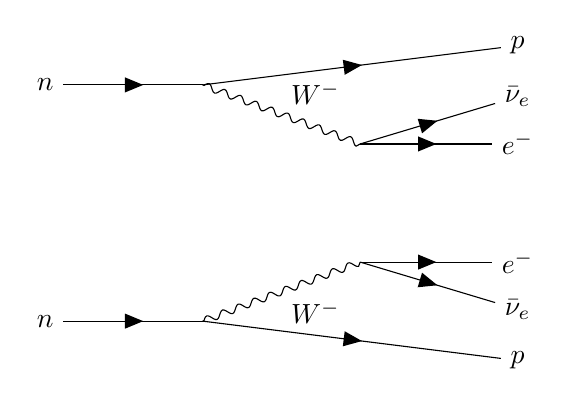
\begin{tikzpicture}
    \begin{feynman}
      \vertex (n1) at (0, 1.5) {$n$};
      \vertex (n2) at (0,-1.5) {$n$};
      \vertex (v1) at (2, 1.5);
      \vertex (v2) at (2,-1.5);
      \vertex (w1) at (4, 0.75);
      \vertex (w2) at (4,-0.75);
      \vertex (p1) at (6, 2.0) {$p$};
      \vertex (p2) at (6,-2.0) {$p$};
      \vertex (e1) at (6, 0.75) {$e^-$};
      \vertex (e2) at (6,-0.75) {$e^-$};

      % antineutrino external legs (place them a bit to the left of the W vertices)
      \vertex (nu1) at (6, 1.35) {$\bar{\nu}_e$};
      \vertex (nu2) at (6,-1.35) {$\bar{\nu}_e$};

      \diagram* {
        (n1) -- [fermion] (v1) -- [fermion] (p1),
        (n2) -- [fermion] (v2) -- [fermion] (p2),
        (v1) -- [boson, edge label=$W^-$] (w1),
        (v2) -- [boson, edge label'=$W^-$] (w2),

        (w1) -- [fermion] (e1),
        (w2) -- [fermion] (e2),

        % outgoing antineutrinos
        (w1) -- [fermion] (nu1),
        (w2) -- [fermion] (nu2),
      };
    \end{feynman}
  \end{tikzpicture}
  \end{minipage}
  \hfill
  \begin{minipage}{0.45\textwidth}
  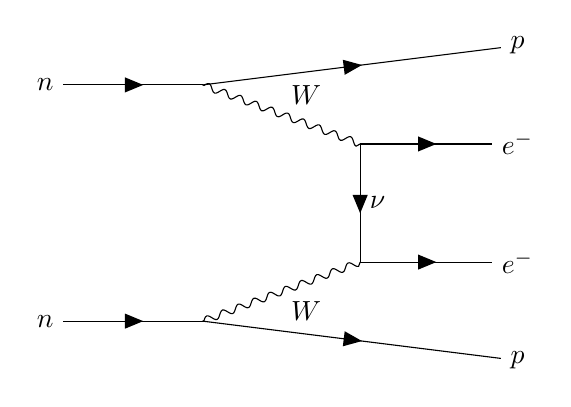
\begin{tikzpicture}
    \begin{feynman}
      \vertex (n1) at (0,1.5) {$n$};
      \vertex (n2) at (0,-1.5) {$n$};
      \vertex (v1) at (2,1.5);
      \vertex (v2) at (2,-1.5);
      \vertex (w1) at (4,0.75);
      \vertex (w2) at (4,-0.75);
      \vertex (p1) at (6,2) {$p$};
      \vertex (p2) at (6,-2) {$p$};
      \vertex (e1) at (6,0.75) {$e^-$};
      \vertex (e2) at (6,-0.75) {$e^-$};
      
      \diagram* {
        (n1) -- [fermion] (v1) -- [fermion] (p1),
        (n2) -- [fermion] (v2) -- [fermion] (p2),
        (v1) -- [boson, edge label=$W$] (w1) -- [fermion] (e1),
        (v2) -- [boson, edge label'=$W$] (w2) -- [fermion] (e2),
        (w1) -- [fermion, edge label=$\nu$] (w2),
      };
    \end{feynman}
  \end{tikzpicture}
  \end{minipage}
  \caption{Feynman diagrams for $2\nu\beta\beta$ decay (left) and $0\nu\beta\beta$ decay (right).}
  \label{fig:feynman_double_beta}
\end{figure}

Under the assumption that light Majorana neutrino exchange dominates, the inverse half-life for $0\nu\beta\beta$ decay can be written in factorized form as:
\begin{equation}
    \left(T^{0\nu}_{1/2}\right)^{-1}
    =
    G^{0\nu}(Q_{\beta\beta}, Z)
    \left| \mathcal{M}^{0\nu} \right|^2
    \left( \frac{m_{\beta\beta}}{m_e} \right)^2 
\end{equation}
where $G^{0\nu}$ is the phase-space factor, $\mathcal{M}^{0\nu}$ is the nuclear matrix element, $m_e$ is the electron mass, and $m_{\beta\beta}$ is the effective Majorana neutrino mass:

\begin{equation}
    m_{\beta\beta}
    =
    \left|
        m_1 U_{e1}^2
        +
        m_2 U_{e2}^2 e^{2 i \xi_1}
        +
        m_3 U_{e3}^2 e^{2 i \xi_2}
    \right| 
\end{equation}


\noindent Here, $m_i$ are the light neutrino mass eigenvalues, $U_{ei}$ are elements of the PMNS mixing matrix, and $\xi_i$ are the Majorana CP-violating phases. Unlike neutrino oscillation experiments, which are insensitive to the absolute mass scale and Majorana phases, $0\nu\beta\beta$ decay probes both. The unknown values of the Majorana phases lead to allowed bands for $m_{\beta\beta}$ as a function of the lightest neutrino mass, with distinct regions corresponding to normal and inverted mass orderings. As a result, experimental limits on the $0\nu\beta\beta$ half-life translate into ranges of allowed $m_{\beta\beta}$ values rather than a single constraint which is illustrated in Figure~\ref{fig:lobster}.

\begin{figure}[tt!]
    \centering
    \includegraphics[width = \textwidth]{2_Chapter_Theory/Figures/lobster_full.jpeg}
    \caption[Possible Majorana masses for normal (magenta) and inverted (blue) mass orderings, calculated with mixing angles and mass differences from the PMNS matrix.]{Possible Majorana masses for normal (magenta) and inverted (blue) mass orderings, calculated with mixing angles and mass differences from the PMNS matrix. The error bands come from uncertainties in the mixing parameters~\cite{Esteban_2024}. The KamLAND-Zen experimental limit on \(m_{\beta\beta}\) is shown in gray.  Recent limits~\cite{PhysRevLett.125.252502,PhysRevLett.126.181802,PhysRevLett.129.222501} for other key isotopes are shown in the panel on the right. Figure taken from Reference~\cite{DGooding2025}.}\label{fig:lobster}
\end{figure}

While the phase-space factor $G^{0\nu}$ can be calculated with high precision, the NME $\mathcal{M}^{0\nu}$ remains the largest source of theoretical uncertainty in interpreting $0\nu\beta\beta$ searches. The calculation of $\mathcal{M}^{0\nu}$ requires detailed knowledge of nuclear wave functions and many-body correlations and depends on the treatment of short-range physics, nuclear deformation, and the effective axial-vector coupling.  For the standard light Majorana neutrino exchange mechanism, the NME can be written schematically as a sum of long- and short-range contributions:
\begin{equation}
    \mathcal{M}^{0\nu}_{\mathrm{light}}
    =
    g_A^4
    \left(
        \mathcal{M}^{0\nu}_{\mathrm{long}} + \mathcal{M}^{0\nu}_{\mathrm{short}}
    \right)
\end{equation}
The axial-vector coupling constant $g_A$ governs the long-range weak interaction of nucleons and is factored out explicitly, serving as an important parameter in nuclear many-body calculations. The short-range contribution depends additionally on a two-nucleon coupling, $g^{\mathrm{NN}}$, which is not written explicitly here. As in the case of $2\nu\beta\beta$ decay, the phase-space factors relevant for $0\nu\beta\beta$ are known with high precision for all experimentally relevant isotopes~\cite{Kotija2012,Horoi2018}. In contrast, the NMEs themselves, along with some associated hadronic couplings, remain a dominant source of theoretical uncertainty despite significant recent progress.

The nuclear matrix elements (NMEs) encode the influence of nuclear structure on the rate of neutrinoless double beta decay and are obtained by combining nuclear wave functions for the initial and final states with the appropriate transition operators. In practice, NMEs are evaluated using nuclear many-body methods that attempt to capture correlations among nucleons across a wide range of length and energy scales. When limits on the $0\nu\beta\beta$ half-life are translated into constraints on the effective Majorana mass $m_{\beta\beta}$, the resulting uncertainty is presently dominated by the spread in available NME calculations rather than by experimental systematics.  A detailed theoretical treatment of the construction of the transition operators, the treatment of short-range correlations, and the associated theoretical uncertainties lies beyond the scope of this thesis. Comprehensive reviews of modern NME calculations can be found in Reference~\cite{Engel_2017}.

In general, NME calculations proceed by first specifying an effective nuclear Hamiltonian that includes nucleon--nucleon interactions relevant to the decay process. A second step then introduces a framework for describing collective nuclear structure and many-body correlations beyond the mean-field level. The most widely used approaches are summarized below.

\begin{itemize}

\item The \textbf{Nuclear Shell Model (NSM)} has long served as a foundational tool for describing nuclear structure. In this framework, nucleons are treated as moving independently within a mean-field potential, augmented by a strong spin--orbit interaction. This potential, often modeled using harmonic oscillator or Woods--Saxon forms, represents the averaged interaction of a nucleon with the rest of the nucleus. The resulting single-particle states organize into energy shells, with particularly stable configurations occurring at so-called magic numbers. For practical calculations, the nucleus is typically separated into an inert core of filled shells and a smaller set of active valence nucleons. While the shell model provides a highly detailed description of nuclear correlations within the chosen model space, computational limitations restrict its applicability to relatively small valence spaces.

\item The \textbf{Quasiparticle Random Phase Approximation (QRPA)} extends mean-field approaches by incorporating collective excitations and pairing correlations across a large set of nuclear orbitals. It is particularly well suited for medium and heavy nuclei, where shell-model calculations become computationally prohibitive. QRPA calculations rely on effective proton--neutron interactions, commonly parameterized by the coupling strength $g_{pp}$, which governs proton--neutron pairing. This parameter is often constrained by requiring agreement with experimentally measured $2\nu\beta\beta$ decay rates and subsequently applied to predictions of $0\nu\beta\beta$ decay. As a result, QRPA provides an explicit link between two-neutrino and neutrinoless decay calculations.

\item \textbf{Energy Density Functional (EDF)} methods describe nuclei using energy functionals that depend on local densities and currents, extending the concept of mean-field theory in a self-consistent manner. These methods allow for the inclusion of important nuclear effects such as deformation, pairing, configuration mixing, and collective motion. EDF calculations have proven effective in describing medium and heavy nuclei, which are of primary interest for double beta decay searches. However, EDF-based NMEs are often among the largest reported values, in part because certain proton--neutron correlations are not treated explicitly.

\item The \textbf{Interacting Boson Model (IBM)} provides a simplified, phenomenological description of nuclear structure by mapping pairs of valence nucleons onto bosonic degrees of freedom. In the context of double beta decay, the IBM has been extended to distinguish between proton and neutron bosons (IBM-2), enabling calculations of NMEs for even--even nuclei. While the model sacrifices microscopic detail, it offers a computationally efficient framework for exploring systematic trends across isotopic chains.

\item \textbf{\emph{Ab initio}} methods aim to describe nuclei starting from fundamental interactions derived from quantum chromodynamics via chiral effective field theory. These methods treat all nucleons explicitly and employ nuclear Hamiltonians with minimal phenomenological input. A key advantage of ab initio calculations is their systematic improvability and the ability to assess convergence. While these methods successfully reproduce properties of light and some medium-mass nuclei, extending them to the heavy nuclei relevant for $0\nu\beta\beta$ decay remains an active area of research~\cite{PhysRevLett.126.042502}.

\end{itemize}

\noindent To illustrate the level of agreement among different approaches, Figure~\ref{fig:NMEs} summarizes recent NME calculations for several candidate $0\nu\beta\beta$ isotopes. For a given nucleus, the predicted NMEs typically vary by factors of two to three across models. This spread constitutes one of the primary theoretical limitations in extracting neutrino mass information from $0\nu\beta\beta$ decay searches and provides strong motivation for experimental probes, such as two-neutrino double beta decay to excited states, that can help benchmark and constrain nuclear structure calculations.

\begin{figure}[t!]
	\centering
	\includegraphics[scale=0.6]{NME_calculations.png}
	\caption{Results from various NME calculation of $M_{0\nu}$ on particular \0nbb decaying isotopes versus atomic mass. Figure taken from Reference~\cite{Engel_2017}.}
	\label{fig:NMEs}
\end{figure}



Current nuclear structure methods yield values of $\mathcal{M}^{0\nu}$ that differ by factors of two to three for the same isotope. These discrepancies directly propagate into uncertainties on the extracted limits or measurements of $m_{\beta\beta}$. As a result, the physics reach of $0\nu\beta\beta$ experiments is no longer limited solely by exposure or background reduction, but increasingly by the reliability of nuclear matrix element calculations. Reducing these uncertainties has therefore become a central goal in the field.

\section{Double Beta Decay to Excited States}

An additional class of processes can provide valuable experimental input into NME calculations and aid in the interpretation of $0\nu\beta\beta$ decay searches: two-neutrino double beta decay to excited states of the daughter nucleus, denoted $2\nu\beta\beta^*$. In these Standard Model–allowed transitions, the parent nucleus undergoes double beta decay but populates an excited state of the daughter rather than its ground state. The subsequent de-excitation of the daughter nucleus produces a characteristic gamma-ray cascade.

Decays to excited states are suppressed by several orders of magnitude relative to ground-state transitions due to the reduced available phase space arising from the smaller effective $Q$ value~\cite{exstate_stats}. As a consequence, theoretical predictions for the corresponding half-lives span multiple orders of magnitude, reflecting the same nuclear-structure uncertainties that dominate predictions for $0\nu\beta\beta$ decay. Figure~\ref{fig:ex_halflife} illustrates representative predictions for $T^{2\nu^*}_{1/2}$ obtained using different nuclear models. An experimental observation of $2\nu\beta\beta^*$ in xenon would therefore provide a powerful constraint on nuclear matrix element calculations and help reduce theoretical uncertainties relevant to $0\nu\beta\beta$ searches.

\begin{figure}[t!]
	\centering
	\includegraphics[scale=1.3]{halflife_pred_ex.jpg}
	\caption{Predictions of $T_{1/2}^{2\nu^*}$ using various NME calculation methods. Figure taken from \cite{exhalflife_calc}.}
	\label{fig:ex_halflife}
\end{figure}

The discussion below follows closely the formalism presented in Ref.~\cite{excited_nme}, which explores the relationship between $2\nu\beta\beta$ and $0\nu\beta\beta$ NMEs within the NSM and the proton–neutron quasiparticle random-phase approximation (pnQRPA). The experimental signature of $2\nu\beta\beta^*$ consists of a standard $2\nu\beta\beta$ decay, followed (after a delay of order picoseconds) by the emission of one or more gamma rays as the daughter nucleus relaxes to its ground state. Experimentally, identifying this process requires either particle identification techniques capable of tagging the de-excitation gamma rays or the observation of distortions in the electron energy spectrum relative to the dominant ground-state $2\nu\beta\beta$ background. While challenging, these signatures provide additional handles for background discrimination compared to ground-state decays.

As mentioned in Section~\ref{sec:2vbb} the half-life for $2\nu\beta\beta$ decay can be reasonably approximated with a single nuclear matrix element~\cite{excited_nme}:
\begin{equation}
    \mathcal{M}^{2\nu}
    =
    -\sum_k
    \frac{
        \bigl( 0_f^+ \bigl\| \sum_a \tau_a^- \sigma_a \bigr\| 1_k^+ \bigr)
        \bigl( 1_k^+ \bigl\| \sum_b \tau_b^- \sigma_b \bigr\| 0_i^+ \bigr)
    }{
        \left[ E_k - (E_i + E_f)/2 \right] / m_e
    }
\end{equation}
where the indices $a$ and $b$ run over all nucleons, $\tau^-$ is the isospin-lowering operator converting neutrons into protons, and $\sigma$ is the spin operator. The sum extends over all intermediate $1^+$ states of the odd–odd nucleus, with the energy denominator involving the excitation energy of each intermediate state relative to the average of the initial and final nuclear energies.

In contrast, the $0\nu\beta\beta$ nuclear matrix element (assuming the standard light Majorana neutrino exchange mechanism) is conventionally decomposed into three spin–isospin components:
\begin{equation}
    \mathcal{M}^{0\nu}_L
    =
    \mathcal{M}^{0\nu}_{GT}
    -
    \mathcal{M}^{0\nu}_{F}
    +
    \mathcal{M}^{0\nu}_{T},
\end{equation}
corresponding to Gamow--Teller ($GT$), Fermi ($F$), and tensor ($T$) contributions. These components are defined in terms of two-body operators:
\begin{equation}
    \mathcal{M}^{0\nu}_K
    =
    \sum_{k,ab}
    \bigl(
        0_f^+
        \bigl\|
        \mathcal{O}^K_{ab}
        \tau^-_a \tau^-_b
        H_K(r_{ab})
        f^2_{\mathrm{SRC}}(r_{ab})
        \bigr\|
        0_i^+
    \bigr)
\end{equation}
where $\mathcal{O}^F_{ab}=\mathds{1}$, $\mathcal{O}^{GT}_{ab}=\sigma_a\cdot\sigma_b$, and
\[
\mathcal{O}^T_{ab}
=
3(\sigma_a\cdot\hat{r}_{ab})(\sigma_b\cdot\hat{r}_{ab})
-
\sigma_a\cdot\sigma_b 
\]
The quantity $r_{ab}$ denotes the distance between nucleons $a$ and $b$, and $f_{\mathrm{SRC}}(r)$ accounts for short-range correlations.

The neutrino potential $H_K(r_{ab})$ encodes the momentum dependence of the virtual neutrino exchange and is given by:
\begin{equation}
    H_K(r_{ab})
    =
    \frac{2R}{\pi g_A^2}
    \int_0^\infty
    \frac{
        h_K \, j_\lambda(p r_{ab}) \, p^2 \, dp
    }{
        \epsilon_K
    },
\end{equation}
where $\epsilon_K = p \left[ p + E_k - (E_i + E_f)/2 \right]$, $g_A = 1.27$, and $R = 1.2 A^{1/3}$~fm. The structure of this potential introduces a characteristic radial dependence into the NME, allowing the matrix elements to be expressed in terms of radial distributions:
\begin{equation}
    M^{0\nu}_L(1b)
    =
    \int_0^\infty C^{0\nu}(r)\,dr,
    \qquad
    M^{2\nu}
    =
    \int_0^\infty C^{2\nu}(r)\,dr.
\end{equation}
For $0\nu\beta\beta$ decay, the radial distribution may be decomposed as:
\begin{equation}
    C^{0\nu}(r)
    =
    C^{0\nu}_{GT}(r)
    -
    C^{0\nu}_{F}(r)
    +
    C^{0\nu}_{T}(r),
\end{equation}
with:
\begin{equation}
    C^{0\nu}_K(r)
    =
    \sum_{k,ab}
    \bigl(
        0_f^+
        \bigl\|
        \mathcal{O}^K_{ab}
        \tau^-_a \tau^-_b
        H_K(r_{ab})
        f^2_{\mathrm{SRC}}(r_{ab})
        \delta(r - r_{ab})
        \bigr\|
        0_i^+
    \bigr).
\end{equation}

\noindent Reference~\cite{Jokiniemi:2022ayc} demonstrated that the radial distributions $C^{2\nu}(r)$ and $C^{0\nu}(r)$ exhibit striking qualitative similarities across a wide range of nuclei and model assumptions. Figure~\ref{fig:nme_radial} shows representative radial distributions for $^{76}$Ge calculated within the pnQRPA framework. The similarity in the spatial structure of the two matrix elements suggests that both processes probe related nuclear correlations, despite their different momentum transfers.

\begin{figure}[b!]
	\centering
	\includegraphics[scale=0.35]{nme_radial.png}
	\caption{Radial distributions of \0nbb (top) and \2nbb (bottom) NMEs of $^{76}$Ge obtained via pnQRPA. Figure taken from Reference~\cite{excited_nme}.}
	\label{fig:nme_radial}
\end{figure}

While neither $2\nu\beta\beta$ nor $2\nu\beta\beta^*$ decay rates are accurately predicted \emph{a priori} by nuclear models, strong correlations between $2\nu\beta\beta$ and $0\nu\beta\beta$ NMEs have been observed. In practice, calculated $2\nu\beta\beta$ NMEs are often renormalized using an effective axial coupling to reproduce measured half-lives. Despite this adjustment, the relative trends among isotopes remain robust.

Figure~\ref{fig:corr_2nu_0nu} illustrates the correlation between $2\nu\beta\beta$ and $0\nu\beta\beta$ NMEs obtained using both NSM and pnQRPA calculations. The presence of a clear correlation across different nuclear models supports the idea that improved experimental constraints on $2\nu\beta\beta$, and especially on the more selective $2\nu\beta\beta^*$ transitions, can provide meaningful benchmarks for nuclear structure calculations relevant to $0\nu\beta\beta$ decay.

\begin{figure}[t!]
	\centering
	\includegraphics[scale=0.33]{corr_2nu_0nu.png}
	\caption{Correlation of \2nbb and \0nbb NME as calculated by NSM (Nuclear Shell Model) and pnQRPA (proton-neutron quasiparticle random-phase approximation) methods. Figure taken from Reference~\cite{exstate_corr}.}
	\label{fig:corr_2nu_0nu}
\end{figure}

These theoretical insights provide strong motivation for experimental searches for $2\nu\beta\beta$ to excited states. Such measurements offer a unique opportunity to test nuclear many-body methods, constrain NME calculations, and ultimately improve the reliability of neutrino mass limits extracted from $0\nu\beta\beta$ decay experiments.



% \section{Double Beta Decay to Excited States}
% A related physics process can provide further experimental input into the NME calculations, and aid in the interpretation of \0nbb experiment results, \2nbb to excited states, or \2nbb$^*$. \2nbb$^*$ is a SM process in which the parent isotope undergoes double-beta decay but transitions to an excited state of the daughter nucleus instead of the ground state. These decays are suppressed by orders of magnitude compared to decays to ground states because of the reduced phase space from smaller $Q$ values\cite{exstate_stats}. Mirroring the status of NME calculations, predictions for the decay rates into excited states vary by multiple orders of magnitude, see Figure \ref{fig:ex_halflife}. An observation of this decay in Xenon could inform NME calculations and reduce the theoretical uncertainties. The following discussion of the relationship between \2nbb and \0nbb NMEs follows \cite{excited_nme} closely. This discussin describes how the two calculations are related in the nuclear shell model (NSM) and proton-neutron quasiparticle random-phase approximation (pnQRPA) frameworks.

% \begin{figure}[b!]
% 	\centering
% 	\includegraphics[scale=1.3]{halflife_pred_ex.jpg}
% 	\caption{Predictions of $T_{1/2}^{2\nu^*}$ using various NME calculation methods. Figure taken from \cite{exhalflife_calc}.}
% 	\label{fig:ex_halflife}
% \end{figure}

% The physical signature of \2nbb$^*$ is of a \2nbb decay immediately, few pico-second delay, followed by a gamma cascade as the daughter nucleus relaxes into its ground state. The task of detecting this rare process becomes one of either particle identification or resolving a distortion in the much larger decay to ground state background.

% The \2nbb decay half-life, to a very good approximation, depends on a single NME \cite{excited_nme}.
% \begin{equation}
%     M^{2\nu}=-\sum_k\frac{(0^+_f||\sum_a\tau^-_a\sigma_a||1^k_+)(1^k_+||\sum_b\tau^-_b\sigma_b||0^+_i)}{[E_k-(E_i+E_f)/2]/m_e}
% \end{equation}
% where $a$ and $b$ indices run over all nucleons, the isospin operator $\tau^-$ turns neutrons into protons, $\sigma$ is the spin operator, and the denominator involves the energies of the initial, final, and each $kth$ intermediate $1^+$ state. For \0nbb, considering the best motivated light neutrino exchange mechanism, the NME is usually written in terms of three spin structures:
% \begin{equation}
%     M^{0\nu}_L=M^{0\nu}_{GT}-M^{0\nu}_F+M^{0\nu}_T
% \end{equation}
% The three spin structures are referred to Gamow-Teller ($M^{0\nu}_{GT}$), Fermi ($M^{0\nu}_{F}$), and tensor ($M^{0\nu}_{T}$). They correspond to the operators $\mathcal{O}^F_{ab}=\mathds{I}$, $\mathcal{O}^{GT}_{ab}=\sigma_a\cdot\sigma_b$, $\mathcal{O}^T_{ab}=3(\sigma_a\cdot\hat{r}_{ab})(\sigma_b\cdot\hat{r}_{ab})-\sigma_a\cdot\sigma_b$ used in their definitions:
% \begin{equation}
%     M^{0\nu}_K=\sum_{k, ab} (0^+_f||\mathcal{O}^K_{ab}\tau^-_a\tau^-_bH_K(r_{ab})f^2_{SRC}(r_{ab})||0^+_i)
% \end{equation}
% A factor to note here is $r_{ab}$ the distance between nucleon $a$ and nucleon $b$. Used in the neutrino potential:
% \begin{equation}
%     H_K(r_{ab})=\frac{2R}{\pi g^2_A}\int_0^\infty\frac{h_Kj_\lambda(pr_{ab})p^2dp}{\epsilon_K}
% \end{equation}
% with $\epsilon_K=p(p+E_k-(E_i+E_f)/2)$, $g_A=1.27$, and $R=1.2A^{1/3}$fm
% with nucleon number, $A$. It is in these radial distributions, that give the neutrino potentials structure, that the relationship between \0nbb and \2nbb can be explored.

% We note that the NME radial distributions are qualitatively similar and that they satisfy:
% \begin{equation}
%     M^{0\nu}_L(1b)=\int^\infty_0 C^{0\nu}(r)dr
% \end{equation}
% satisfy:
% \begin{equation}
%     M^{2\nu}=\int^\infty_0 C^{2\nu}(r)dr
% \end{equation}
% Once again we can split the integral into three terms.
% \begin{equation}
%     C^{0\nu}(r)=C^{0\nu}_{GT}(r)-C^{0\nu}_F(r)+C^{0\nu}_T(r)
% \end{equation}
% \begin{equation}
%     C^{0\nu}_K=\sum_{k,ab}(0^+_f||\mathcal{O}^K_{ab}\tau^-_a\tau^-_bH_K(r_{ab})f^2_{SRC}(r_{ab})\delta(r-r_{ab})||0^+_i)
% \end{equation}
% Jokineimi et.al. found a strong correlation in the radial distributions of \2nbb and \0nbb nuclear matrix elements.

% \begin{figure}[b!]
% 	\centering
% 	\includegraphics[scale=0.4]{nme_radial.png}
% 	\caption{Radial distributions of \0nbb (top) and \2nbb (bottom) NMEs of $^{76}$Ge obtained via pnQRPA. Figure taken from \cite{excited_nme}.}
% 	\label{fig:nme_radial}
% \end{figure}

% While neither \2nbb or \2nbb$^*$ has had their decay rates successfully predicted. In fact, the simplest model NMEs are usually adjusted with a "quenching" factor to match the observations of \2nbb half-lives. Without these quenching factors, the models consistently overpredict the half-lives. Close correlation between the NMEs of \2nbb and \0nbb have been demonstrated. Figure \ref{fig:corr_2nu_0nu} shows the correlations between \2nbb and \0nbb NME as calculated by two different methods.

% \begin{figure}[h]
% 	\centering
% 	\includegraphics[scale=0.3]{corr_2nu_0nu.png}
% 	\caption{Correlation of \2nbb and \0nbb NME as calculated by NSM (Nuclear Shell Model) and pnQRPA (proton-neutron quasiparticle random-phase approximation) methods. Figure taken from \cite{exstate_corr}.}
% 	\label{fig:corr_2nu_0nu}
% \end{figure}

% These theoretical findings motivates a better understanding of \2nbb and \2nbb$^*$ to aid in theoretical calculations of $M^{0\nu}$, and determination of Majorana neutrino mass.


% \section{Double Beta Decay Experiments}
% \0nbb if it exists has an incredibly long half-life greater than $10^{26}$ years. Should it be discovered, \0nbb would be the slowest natural process observed experimentally. To successfully carry out this rare event search, \0nbb experiments must be designed with crucial criteria in mind:
% \begin{itemize}
% 	\item \textbf{High Energy Resolution:} Distinguishing the \0nbb peak at the \2nbb endpoint requires precise energy resolution to reduce ROI (region of interest) contamination from the \2nbb decay spectrum. Modern experiments on the forefront of this design criterion are achieving $\frac{\sigma_E}{E}\approxeq 0.1\%$ resolution, and completely suppressing the \2nbb background. 
% 	\item \textbf{High Isotope Loading:} Maximizing the amount of double-beta decaying isotoped in the sensitive regions of the experiment is crucial for achieving sensitivity to long \0nbb half-lives in a reasonable timeframe, usually a decade of data-taking. Modern experiments are instrumenting about a metric ton of double-beta decaying isotope. The limiting factor to this criterion is often budgetary or enrichment capability.
% 	\item \textbf{Low Unrelated Backgrounds:} Experiments need to be prepared in environments with low incidental radioactivity. This necessarily means deep underground facilities, with the experiments themselves being constructed with the highest standard of radiopure materials.
% \end{itemize}
% The current world leading limit on Majorana neutrino mass has been set by KamLAND-ZEN at $m_{\beta\beta} < (28-122) $ meV, at 90\% C.L. The limits on majorana neutrino mass based on multiple NME calculations can be seen in Figure \ref{fig:klz_0nu_limit}. It is readily apparent that the exact values of the NMEs drastically impact the significance of the latest experimental results. For the highest NMEs, the limits placed by KamLAND-ZEN enter the non-degnerate regions of inverted ordering phase space. While for the lower NMEs, the limits remain in the degenerate region. KamLAND-ZEN is the only \0nbb experiment to place limits in the inverted ordering region for any NME.

\section{Double Beta Decay Experiments}

If neutrinoless double beta decay ($0\nu\beta\beta$) exists, it is an extraordinarily rare process, with an expected half-life exceeding $10^{26}$~years for the most favorable isotopes. A confirmed observation would represent the slowest natural radioactive decay ever measured and would provide direct evidence for lepton number violation and the Majorana nature of neutrinos. The extreme rarity of this process imposes stringent requirements on experimental design. Successful $0\nu\beta\beta$ searches must simultaneously maximize signal efficiency while suppressing backgrounds to unprecedented levels. Several key criteria therefore define the performance of modern double beta decay experiments:

\begin{itemize}
	\item \textbf{Excellent Energy Resolution:}  
	The experimental signature of $0\nu\beta\beta$ is a monoenergetic peak at the decay $Q$ value, coincident with the endpoint of the continuous $2\nu\beta\beta$ spectrum. Precise energy resolution is essential to minimize contamination from the $2\nu\beta\beta$ tail within the region of interest (ROI). State-of-the-art experiments now achieve fractional energy resolutions of order $\sigma_E/E \simeq 0.1\%$, effectively eliminating $2\nu\beta\beta$ as a limiting background.

	\item \textbf{Large Isotope Mass:}  
	Sensitivity to extremely long half-lives requires large exposures, motivating the deployment of tonne-scale quantities of double beta decaying isotopes. Achieving such isotope masses typically demands both isotopic enrichment and scalable detector technologies. In practice, enrichment cost and isotope availability often set the ultimate experimental scale.

	\item \textbf{Ultra-Low Background Environment:}  
	Backgrounds from natural radioactivity and cosmic-ray interactions must be suppressed to levels below one count per tonne-year in the ROI. This necessitates operation in deep underground laboratories, stringent material screening, and detector designs that enable powerful background discrimination.
\end{itemize}

\noindent Among current-generation experiments, KamLAND-Zen has demonstrated world-leading sensitivity to $0\nu\beta\beta$ decay in $^{136}$Xe. The most recent KamLAND-Zen result places a 90\% confidence level limit on the effective Majorana neutrino mass of $m_{\beta\beta} < (28\text{--}122)\ \text{meV},$ where the range reflects uncertainties associated with NME calculations. Figure~\ref{fig:klz_0nu_limit} shows the corresponding constraints in the $m_{\beta\beta}$–$m_{\text{lightest}}$ plane for multiple NME models. The figure highlights the critical role of nuclear theory: for larger NMEs, the KamLAND-Zen limit begins to probe the non-degenerate region of the inverted neutrino mass ordering, whereas for smaller NMEs the constraint remains within the quasi-degenerate regime. KamLAND-Zen is currently the only $0\nu\beta\beta$ experiment whose sensitivity reaches the inverted-ordering parameter space for any NME calculation.


\begin{figure}[t!!]
	\centering
	\includegraphics[scale=0.35]{klz_0nu_limit.png}
	\caption{Effective Majorana neutrino mass as a function of the lightest neutrino mass state $m_{lightest}$. The shaded regions are based on best-fit values of neutrino oscilation parameters for (a) the normal ordering (NO) and (b) the inverted ordering (IO), the lighter shaded regions indicate the $3\sigma$ ranges based on oscillation parameter uncertainties. The horizontal lines indicate 90\% C.L. limits on $m_{\beta\beta}$ considering multiple NME calculations. Figure taken from Reference~\cite{full_klz_0nu}.}
	\label{fig:klz_0nu_limit}
\end{figure}


Two-neutrino double beta decay to excited states ($2\nu\beta\beta^*$) has been experimentally observed in only a small subset of known double beta decay isotopes. To date, positive detections have been reported for just two transitions:
\begin{itemize}
    \item $^{100}$Mo $\rightarrow\,^{100}$Ru$(0^+_1)$, with
    $T_{1/2} = 5.9^{+0.9}_{-0.6}\times10^{20}$~years,
    \item $^{150}$Nd $\rightarrow\,^{150}$Sm$(0^+_1)$, with
    $T_{1/2} = 1.33^{+0.45}_{-0.26}\times10^{20}$~years.
\end{itemize}

\noindent The scarcity of observed $2\nu\beta\beta^*$ transitions reflects the substantial experimental challenges associated with these decays. Relative to ground-state $2\nu\beta\beta$, decays to excited states suffer from significantly reduced phase space and therefore much longer half-lives. However, their distinctive experimental signature, characterized by the coincident emission of de-excitation gamma rays, offers additional handles for background suppression and provides a powerful probe of nuclear structure.

To date, $2\nu\beta\beta^*$ decay has not been observed in $^{136}$Xe, the isotope used by KamLAND-Zen and the primary focus of this thesis. The current most stringent limit on this process:
\[
T^{2\nu}_{1/2}(0^+ \rightarrow 0^+_1) > 1.4\times10^{24}\ \text{years} \quad (90\%~\text{C.L.})
\]
was established by the EXO-200 experiment~\cite{exo200}. Figure~\ref{fig:exo200_fit} shows the EXO-200 spectral fits used to extract this limit. No statistically significant excess consistent with an excited-state signal was observed.

The analysis presented in this dissertation reports the latest search for $2\nu\beta\beta^*$ using KamLAND-Zen~800 data. Leveraging KamLAND-Zen’s large $^{136}$Xe mass, low background environment, and excellent energy resolution, this work achieves sensitivity beyond the existing EXO-200 limit. An improved constraint on $2\nu\beta\beta^*$ decay in $^{136}$Xe would provide an important experimental benchmark for NME calculations and directly inform the interpretation of current and future $0\nu\beta\beta$ searches.


% \subsection{Observations and Current Limits of $2\nu\beta\beta^*$}
% Double beta decay to excited states has been observed in only two isotopes, a minority of the isotopes known to undergo double-beta decay.
% \begin{itemize}
%     \item $^{100}Mo-^{100}Ru(0^+_1)$ : $T_{1/2}=5.9^{+0.9}_{-0.6}\times 10^{20}$ years
%     \item $^{150}Nd-^{150}Sm(0^+_1)$ : $T_{1/2}=1.33^{+0.45}_{-0.26}\times 10^{20}$ years
% \end{itemize}
% \2nbb$^*$ has yet to be observed in $^{136}Xe$ the double beta decaying isotope of the KamLAND-ZEN experiment and the focus of this thesis. The current world-leading limit on this process is $T^{2\nu}_{1/2}(0^+\rightarrow 0^+_1)>1.4\times 10^{24}$ years at 90\% C.L. set by the EXO-200 experiment. This work describes the latest analysis of KamLAND-ZEN 800 data which surpasses this limit.

\begin{figure}[b!]
	\centering
	\includegraphics[scale=0.42]{exo200_fit.png}
	\caption{EXO-200's fit over energy spectrum (left) and particle ID discriminator spectrum (right) in two data-taking phases of the excited state signal and background. The decay to excited states was not found, and a lower limit was placed. Figure taken from \cite{exo200}.}
	\label{fig:exo200_fit}
\end{figure}
\cleardoublepage

\chapter{The KamLAND-Zen Experiment}
\label{chapter:klz-detector}
\thispagestyle{myheadings}
\graphicspath{{3_Chapter_KLZ_Detector/Figures/}}

KamLAND, the \textbf{Kam}ioka \textbf{L}iquid-scintillator \textbf{A}nti Neutrino \textbf{D}etector, is a large liquid scintillator calorimeter detector situated 1km below mt. Ikenoyama in Gifu prefecture, Japan. I will describe the KamLAND detector's and the corresponding KamLAND experimental area's important components and features in this chapter. I will also explain how each component contributes to the KamLAND's scientific goals and the work of this thesis.


\section{KamLAND}
\label{sec:KamLAND}
One can think of KamLAND as an onion made up of many spherical layers, each layer serving the ultimate goal of shielding and observing the central core, the xenon-loaded liquid scintillator.

\subsection{Detector Infrastructure and Outer Detector}
The KamLAND detector is surrounded by the KamLAND experimental area, situated in an old iron mine, multiple caverns and passageways were excavated and set aside for KamLAND experimental use.

\begin{figure}[htb]
	\centering
	\includegraphics[scale=0.4]{KamLAND_site.png}
	\caption{KamLAND site}
	\label{fig:kamlandsite}
\end{figure}

The KamLAND site is shown in Figure \ref{fig:kamlandsite}. The control room contains networking and monitoring equipment which on-site shifters use to observe real-time detector activity. The first LS purification areas contain liquid-liquid extraction and nitrogen purge purification systems. The second LS purification area contains a distillation purification system. A new Xenon purification area was built for KamLAND-Zen. The dome area is a class 1,000 clean area atop the detector and includes a calibration source preparation room and electronics enclosure (electronics hut or e-hut). At the center of the dome area, there is a secondary class 100-1000 clean tent covering the KamLAND chimney. The inner balloon installations took place in August 2016 and May 2018 inside this clean tent.

The outer detector (OD) is a cylindrical water tank 20m tall and with 20m diameter and filled with pure water. The OD was refurbished in 2016, and 140 new 20-inch PMTs (R3600) were installed inside the cavity. The inner wall of the outer tank and the outer surface of the inner detector stainless steel spherical tank are covered highly reflective Tyvek sheets (Tyvek 1073B and 1082D) to collect as much of the light generated by crossing cosmic ray muons as possible. The outer detector's role is to tag cosmic ray muons, shield radioactivity and fast neutrons from the outer rock, and to stabilize the temperature of the ID.

\subsection{Inner Detector}
KamLAND's inner detector (ID) is the main spherical liquid scintillator detector, it is shown in Figure \ref{fig:kamland}. The ID is contained in a 18m diameter stainless steel sphere tank. 1,879 PMTs are mounted onto the inner wall of the ID, 1,325 17-inch and 554 20-inch PMTs. The PMTs are submerged in non-scintillating buffer oil (BO). An acrylic panel separates the buffer layer into two shells. This panel prevents the convection of radon out-gassed from PMT glasses into the central parts of the detector.

\begin{figure}[htb]
	\centering
	\includegraphics[scale=0.5]{kamland.png}
	\caption{KamLAND-Zen detector}
	\label{fig:kamland}
\end{figure}

Photomultiplier tubes (PMTs) are KamLAND's eyes, detecting individual photons of light emitted by the passage of charged particles through the liquid scintillator volumes. Photons that hit PMT photocathodes are converted into a photoelectron. This photoelectron is then guided by electric fields to a series of dynodes. Each dynode multiplies the photoelectrons many times over, until the first photoelectron becomes $10^{6-7}$ electrons. Should multiple photons hit the photocathode simultaneously, the output voltage increases proportionally. This current is converted to a voltage by a coupling capacitor and read out via long coaxial cables. Figure ~\ref{fig:pmts} is a diagram of the 17in and 20in PMTs.

\begin{figure}[htb]
	\centering
	\includegraphics[scale=0.35]{pmts.png}
	\caption{17-inch and 20-inch PMTs, both have the same footprint, but the 17-inch PMT photocathode is masked to a 17-inch diameter.}
	\label{fig:pmts}
\end{figure}

The 1,325 17-inch PMTs are Hamamatsu R7250s while the 554 20-inch PMTs are Hamamatsu R1449s and R3600s. The 20-inch PMTs were inherited from the Kamiokande experiment to increase our light collection. Both sets of PMTs have a bialkali photocathode sensitive to 300-650nm light which is well-suited for the emission spectrum of the LS. The pmts also differ by dynode design; while the 17-inch PMTs feature "box-and-line" designs, the 20-inch PMTs have "venetian-blind styles". The different dynode designs along with the masking on the 17-inch PMTs, give us 17-in PMTs with better transit time spread (TTS) and 20-inch PMTs with better light collection efficiency. In total, the photocathode coverage of the ID is 34\%, with 23\% contributed by the 17-inch PMTs.

Furthermore, the PMT performance can be affected by the earth's magnetic field. To reduce this unwanted effect, the entire KamLAND detector is surrounded by geomagnetic compensation coils to counteract this external magnetic field. The residual magnetic field is less than 50mG, which has negligible effect on the PMT performance.

Another important characteristic of PMTs is their quantum efficiency (QE). The QE quantifies the probability that a photon arriving on the photocathode will produce a photoelectron. A PMT's QE varies over the wavelength of the incoming light. To improve our light collection, KamLAND's LS is doped with PPO to shift the wavelength of the incoming light to where the PMTs are most sensitive. Figure ~\ref{fig:qe_emission} shows the PMT QE curve and the PPO reemission spectrum.

\begin{figure}[htb]
	\centering
	\includegraphics[scale=0.35]{qe_PPO_emission.png}
	\caption{Quantum Efficiency of the KamLAND inner PMTs and PPO emission over wavelength. Figure taken from \cite{mastuda_phd}}
	\label{fig:qe_emission}
\end{figure}

Next, is the 13m diameter outer balloon (OB). The OB is suspended in the center of the ID within the buffer oil, it is filled with one kiloton of highly purified organic liquid scintillator.

\subsection{Liquid Scintillator}
Liquid scintillator (LS) is the vital medium that sensitizes KamLAND to internal radioactivity. The KamLAND LS (KamLS), found in between the outer balloon and inner balloon, is composed of 80.2\% of dodecane (D12),1,2,4-trimethyl benzene, and 19.8\% pseudocumene (PC). A wavelength shifter called 2,5-diphenyloxazole (PPO) is added to the LS at a concentration of $1.36 \pm 0.03$ g/L. KamLAND-Zen has achieved $5 \times 10^{-18}$ g/g and $1.3 \times 10^{-17}$ g/g contamination for 238U and 232Th, respectively. The chemical composition of the KamLS can be found in Table ~\ref{tbl:kamls}

\begin{table}[h]
	\centering
	\renewcommand{\arraystretch}{1.2}
	\begin{tabular}{c|ccc}
		\hline
		& D12 & PC & PPO \\
		\hline
		Chemical Formula & C$_{12}$H$_{26}$ & C$_9$H$_{12}$ & C$_{15}$H$_{11}$NO \\
		Density [$g/cm^3$] & 0.7526 & 0.8796 & -\\
		Boiling Point [$^\circ$C] & 216 & 169 & 360 \\
		Melting Point [$^\circ$C] & -10 & -44 & 72 \\
		Flash Point [$^\circ$C] & 83 & 54 & - \\ \hline
	\end{tabular}
	\caption{Composition and properties of KamLAND Liquid Scintillator (KamLS)}
	\label{tbl:kamls}
\end{table}

\subsection{KamLAND-Zen and XeLS}
At the center of KamLAND-Zen lies the Xenon-loaded Liquid Scintillator (XeLS) contained in the 1.9m radius inner balloon (IB). The double-beta decaying isotope $^{136}Xe$ is thus placed in the cleanest, most sensitive part of the experiment. The Xenon gas is enriched to 90\% $^{136}Xe$ and is dissolved into a modified version of KamLS. The PPO concentration was increased to 4g/L to boost the light yield. This increased PPO concentration compensates for the 10\% reduction in emitted scintillation light when Xenon is mixed into the LS. The XeLS density is also tuned to match the surrounding KamLS. The chemical composition of the XeLS is shown in Table \ref{tbl:xels} in each of the different phases of the KamLAND-Zen experiment.

\begin{table}[h]
	\centering
	\renewcommand{\arraystretch}{1.2}
	\begin{tabular}{c|cccc}
		\hline
		Material & Decane (\%) & PC (\%) & PPO (\%) & Xe (\%)\\ \hline
		Zen 400 Phase-1 & 82.3 & 17.7 & 2.7 & 2.44/2.48\\
		Zen 400 Phase-2 & 80.7 & 19.3 & 2.29$\pm$0.03 & 2.91\\
		Zen 800 & 82.4 & 17.6 & 2.38$\pm$0.02 & 3.13\\ \hline
	\end{tabular}
	\caption{Composition of XeLS from three phases of KamLAND-ZEN}
	\label{tbl:xels}
\end{table}

\section{Chemical Handling Infrastructure}
Background mitigation is crucial for \0nbb. Maintaining the purity of the liquid volumes inside KamLAND is an important part of background mitigation in KamLAND-Zen. In this section, we will briefly describe the systems that provided or maintain the purity of the LS and XeLS in KamLAND.

\subsection{Water Extraction}
The first purification is shown in Figure ~\ref{fig:waterex}. Both the liquid scintillator and buffer oil are filtered in two stages with 1$\mu$m and 0.1$\mu$m pore sizes respectively. Next, the liquids are flushed with pure water in the water extraction tower where metals such as U, Th, and K, are absorbed by the water. Finally, the liquids are purged with ultra-pure nitrogen gas to remove gaseous contaminants like radon and oxygen.

\subsection{Distillation}
The next purification system utilizes the distillation system shown in Figure ~\ref{fig:distillation}. LS from KamLAND is constantly cycled through the distillation system. There boiling is done to separate the individual chemical components of KamLS, namely Pseudocumene (PC) and PPO. Each component is individually distilled and purified. Then, the components are combined in the mixing tank to the original LS composition with an accuracy of $10^{-3}g/cm^3$. Finally high-purity nitrogen gas is used to purge the LS coming out of the mixing tank to eliminate any gaseous contaminants.

\subsection{Xenon Handling}
A schematic diagram of the XeLS handling system is shown in Figure~\ref{fig:xenonhandling}. The system consists of the following components:
\begin{itemize}
	\item A \textbf{1.1 m$^3$ Main Tank} directly connected to KamLAND-ZEN's inner balloon. The extracted XeLS first enters this tank.
	\item A \textbf{1.1 m$^3$ Reservoir Tank} that is connected to the main tank via a vacuum pump and LS trap. It is refrigerated with liquid N$_2$ to -50$^\circ$C, at which the LS gas is condensed and trapped. Only Xe gas is allowed to flow into the reservoir tank.
	\item A \textbf{25 m$^3$ Storage Tank} is connected to the main tank. The degassed LS is poured into this tank for storage.
	\item A \textbf{1.1 m$^3$ Sub-tank} is also connected to the main tank, the detector, the control tank, and the purified Xe gas system. The Xe gas is mixed into LS inside this tank. The density of chemical cocktails in the sub-tank is monitored and adjusted by the control tank. After mixing, the XeLS is filtered and fed back into the balloon.
	\item A \textbf{1.1 m$^3$ Control Tank} is directly connected to the second purification area. The control tank controls the density in the sub-tank by adjusting the Decane percentage. The control tank is pressurized with Nitrogen gas. 
\end{itemize}

\begin{figure}[htb]
	\centering
	\includegraphics[scale=0.5]{xenonhandling.png}
	\caption{Flow diagram of the KLZ Xenon system. The purple lines denote the flow of Xe/XeLS, the blue line denotes the flow of decane, the the grey line denotes the flow of LS. Figure from Reference }
	\label{fig:xenonhandling}
\end{figure}

\section{Data Acquisition}
\subsection{KamLAND DAQ}
KamLAND uses two data acquisition (DAQ) systems in parallel. The first is KamFEE (KamLAND Front End Electronics), which has been used since the start of KamLAND physics data-taking. The other is MoGURA (Module for General-Use Rapid Application). MoGURA is a data acquisition system developed to eliminate the deadtune just after cosmis ray muon events. An overview of this dual scheme data acquisition system is shown in \ref{fig:kamland_daq}. What follows is a brief description of each DAQ system.

\begin{figure}[htb]
	\centering
	\includegraphics[scale=0.3]{kamdaq_flow.png}
	\caption{Flow diagram of the KamLAND data acquisition system, taken from \cite{li_phd}}
	\label{fig:kamland_daq}
\end{figure}

\subsection{KamFEE DAQ}
KamFEE are the front end electronics that read and control the KamLAND PMTs. The boards are of VME 9U form factor and are synchronized with a 40 MHz clock. The PMT signals are sent along two parallel channels. The first channel is sent to a discriminator which register a PMT hit if the voltage exceeds a predetermined value that corresponds to approximately 1/6th of a single photoelectron. The second channel, is delayed to give some time to process the discriminator signal and is fed into 3 amplifier stages (x20, x4, x0.5), this amplified signal is digitized by two analog Transient Waveform Digitizers (ATWDs). The ATWD is a 10-bit digitizer and samples every 1.5ns, 128 times per waveform. Each pulse takes 128 $\mu$sec to digitize.

The KamFEE boards send a "hitsum" signal to the central KamFEE DAQ trigger, communicating a certain number of hits were received and can be digitized. The trigger board sends a signal back which issues the digitization command to the ATWDs. While the ATWD is digitizing, it cannot record further signals, therefore, two ATWDs are assigned to each channel to reduce deadtime.

\subsection{MoGURA}
MoGURA is the secondary data acquisition system in KamLAND; it is responsible for after pulses and dealing with PMT waveform overshoots caused cosmic muons. KamLAND has a cosmic muon rate of 0.3 Hz, so it is important to compensate for the effects these high-energy events have on our detector. To accomplish this task, MoGDAQ has a few extra features over KamFEE.
\begin{itemize}
	\item \textbf{Baseline Recovery:} After a high energy muon passes through the detector, the DAQ channels are saturated, which means the voltage exceeds the digitization window, so only the maximum value is read. Simultaneously, the voltage "overshoots" as it returns to normal and swings below the nominal value causing difficulties in digitizing signals that occur soon after these muons. 
	\item \textbf{Adaptive mode:} Activates a special trigger mode after muon events to compensate for large after-pulses post-muon. This special trigger is based on differential PMT hits. 
\end{itemize}

MoGURA data is used to tag neutrons created from muon spallation. These tagged spallation neutrons are vital in subsequent analyses to tag events that likely originated from these cosmic ray muons. The baseline restoration and neutron tagging will be further improved with the implementation of MoGURA2 trigger system. This is a planned replacement of the KamLAND data acquisition system (KamFEE and MoGDAQ both) for the KamLAND2-ZEN experiment, which is planned to begin physics data-taking in 2028.

\section{KamLAND-ZEN Phases}
The KamLAND-ZEN experiment has undergone multiple phases and renovations.
\subsection{KamLAND-ZEN 400}
The inner balloon and XeLS was added to the KamLAND experiment in 2011, starting the phase referred to as KamLAND-ZEN 400. This phase of the detector featured a 3m diameter inner-balloon filled with liquid scintillator loaded with 3\% Xenon by weight. The dissolved Xenon gas had 91\% proportion of Xe$^{136}$.

The KamLAND-ZEN 400 data was split into two data-taking periods. Period-I data was contaminated with a high background of Ag$^{110m}$, the silver appeared to be leeching from the mini-balloon into the XeLS. The Ag$^{110m}$ contamination on the inner balloon was likely due to nuclear fallout from the Fukushima reactor meltdown. The Fukushima meltdown occurred when the inner balloon was being manufactured and in the same geographical region of Japan. Period II started after the XeLS distillation suppressed the Ag$^{110m}$ by a facator of 20. Period II continued data taking for 534.5 total livedays and the combined physics result of Periods I and II produced a \0nbb half-life limit of $T_{1/2}^{0\nu}>1.07\times 10^{25}$ years at 90\% C.L. This half-life limit corresponds to an effective majorana mass limit of $m_{\beta\beta} < 61-165$ meV. 

\subsection{KamLAND-Zen 800}
KamLAND-ZEN 800 was the second phase of KamLAND-ZEN. KamLAND-ZEN took data from January 2019 to August 2024. Over 2kton$\cdot$yrs of exposure was observed. KamLAND-ZEN 800 was decommission in Fall 2024, and is currently being dissassembled. \\
\subsection*{Inner Balloon Manufacturing}
KamLAND-ZEN 800 featured a larger, cleaner inner balloon which was fabricated at Tohoku University in a Class 1 cleanroom. The inner balloon is made from panels of 25 $\mu$m nylon-6. Innerballoon fabrication consisted of multiple steps some of these critical steps are listed here:
\begin{itemize}
	\item \textbf{Washing} - the film is cleaned twice in an ultrasonic bathtub, then stored between cover films to prevent dust adhesion
	\item \textbf{Welding} - the cleaned balloon panels are welded with a semi-automatic welding machine. For delicate areas, such as the balloon neck, a hand welding machine was used. The average tensile strength on the balloon surface was 35 $N/cm$ after welding.
	\item \textbf{He Leak Check} - Inevitably leaks will occur during the previous assembly procedures. Helium gas was pumped into the balloon to check for these leaks. The cover film of the balloon was peeled off before this leak check. Found leaks were repaired by patching the film. Over 900 leaks were found during the leak check.
	\item \textbf{Folding} - The inner balloon was folded into a cylinder shape and covered with sheath films to prevent contamination during transport. Teflon sheets and Vectran strings were used to tie the rolled balloon up for shipping.
	\item \textbf{Shipping} - The inner balloon was shipped within a silver gas bag. All corresponding tools were also shipped in airtight bags.
\end{itemize}
The inner balloon was installed on May 10, 2018. A rehearsal installation was performed in a swimming pool before the final deployment. In the final installation, the balloon is deployed through the 50cm port on the neck of the KamLAND detector. After filling the balloon with KamLS, the Teflon sheets, sheath films, and Vectran strings are pulled out of the detector. The whole operation was monitered in real-time via cameras and endoscope.

The top of the inner balloon is connected to a corrugated tbue made from PEEK (poly-ether-ether-ketone). Twelve suspending belts support the inner balloon, wrapping around the full height of the balloon. The tension of each of these belts are monitored in real time to guarantee the position and stability of the balloon. A schematic of the balloon structure can be seen in Figure \ref{fig:balloon_structure}. 

\begin{figure}[htb]
	\centering
	\includegraphics[scale=0.5]{ballonstructure.png}
	\caption{Inner balloon structure and measurements for KamLAND-ZEN 800 configuration, taken from \cite{ozaki_phd}}
	\label{fig:balloon_structure}
\end{figure}


\subsection*{Contamination Control}
Once deployed and exposed to the KamLAND scintillators, the inner balloon is very difficult to clean. Thus, maintaining balloon cleanliness is vital. After deployment, the IB was filled with distilled LS while the $^{232}$Th level was measured at $10^{-15}$g/g, exceeding the target background concentration. The PPO distillation tower was suspected to be a source of contamination and was investigated. ICP-MS and neutron activation analysis were used to measure $^{232}$Th contamination at different locations along the distillation system. After meticulous washing and filter replacement, LS purification began to lower the $^{232}$Th background. After two separate distillation campaigns, $^{238}$U and $^{232}$Th levels were reduced by a factor of 10 compared to KamLAND-ZEN 400. The contaminations can be estimated by performing a $^{214}$Bi-$^{214}$Po and $^{212}$Bi-$^{212}$Po coincidence analysis. The coincidence event rates plotted over time are shown in Figure \ref{fig:coincidence_rate} and listed in Table \ref{tbl:filmcontamination}.

\begin{figure}[htb]
	\centering
	\includegraphics[scale=0.3]{coincidencerate.png}
	\caption{Coincidence event rate in KamLAND-ZEN 800 during the first distillation campaign, second distillation campaign, and Zenon loading phase. The red points denote $^{214}$Bi and the blue points denote $^{212}$Bi. Figure taken from \cite{li_phd}.}
	\label{fig:coincidence_rate}
\end{figure}

\begin{table}[htb]
	\centering
	\renewcommand{\arraystretch}{1.2}
	\begin{tabular}{c|cc}
		\hline
		 & $^{238}$U ($10^{-17}$ g/g) & $^{232}$Th ($10^{-17}$ g/g)\\ \hline
		Zen 400 Phase-1 & 13$\pm$2 & 190$\pm$20 \\
		Zen 400 Phase-2 & 17$\pm$1 & 5.5$\pm$0.3 \\
		Zen 800 & 1.5$\pm$0.4 & 30$\pm$4 \\ \hline
	\end{tabular}
	\caption{Film Contamination three phases of KamLAND-ZEN. Values taken from \cite{ozaki_phd}}
	\label{tbl:filmcontamination}
\end{table}

KamLAND-ZEN 800 was decomissioned in 2024 after observing over 2 kiloton$\cdot$yrs of exposure. The final half-life limit was reported as $T_{1/2}^{0\nu} > 3.8\times 10^{26}$ years at 90\% C.L. This half-life limit corresponds to an effective majorana mass limit range of 28-122 meV. As of Summer 2025, this is the world-leading limit on effective majorana mass from any double-beta decay isotope and is the only limit in the Inverted Mass Ordering region. The latest limits from KamLAND-ZEN800 are shown in Figure \ref{fig:klz800_result}

\begin{figure}[htb]
	\centering
	\includegraphics[scale=0.35]{klz800_result.png}
	\caption{Effective Majorana neutrino mass $m_{\beta\beta}$ as a function of the lightest neutrino mass $m_{lightest}$. The dark shaded regions are based on the best-fit neutrino oscillation parameters, while the lighter regions indicate 3$\sigma$ ranges calculated from oscillation parameter uncertainties \cite{PhysRevD.90.033005} \cite{Nufit}. The horizontal lines indicate various 90\% C.L. upper limits on $m_{\beta\beta}$ from KamLAND-ZEN's $^{136}$Xe results and a few different NME calculations. The blue bars on the right indicate three different theoretical predictions in the IO region. \cite{klz800_arxiv}}
	\label{fig:klz800_result}
\end{figure}

\subsection{KamLAND2-ZEN}
KamLAND2 is the next generation of the KamLAND experiment, it will be built in the same detector cavern as KamLAND1. KamLAND2-ZEN will reach a goal limit of $T_{1/2}^{0\nu\beta\beta}>2\times 10^{27}$ yrs.

Most of the detector components will be replaced going from KamLAND to KamLAND2. Some of the more notable upgrades are:
\begin{itemize}
	\item \textbf{Inner Detector PMTs} - All of the 1,879 inner PMTs will be replaced with modern low-TTS, high quantum efficiency (QE) phototubes. 
	\item \textbf{Light Collecting Mirrors} - Light collecting winston cones will be attached to each of the PMTs to achieve virtually 100\% photocoverage. These improvements will contribute to a goal energy resolution of 2\%. This energy resolution will lead to a x100 reduction in the $2\nu\beta\beta$ background rate.
	\item \textbf{Improved Inner Balloon} - The new innerballon will be made up of PEN (polyethylenenapthalate) which will scintillate from film radioactive backgrounds
	\item \textbf{MoGURA2} - Replace the 2 DAQ systems with MoGURA2, a newly developed, compact, dead-time free, RFSoC electronics.
\end{itemize}
KamLAND2-ZEN is scheduled to begin data-taking in 2028.

% {\bf Important}: You will also be using a lot of citations. The format in this template follows the so-called APA style and looks as follows in the document body: \cite{lamport1985:latex}, \cite{Debr01}. There are no numbers in the list of references -- the list is sorted alphabetically according to the first author's last name.

% Other styles of references are allowed by the library as well, e.g., ``plain'' or ``'ieee'', which use numbers in square brackets both in the document body and in the list of references. In order to use another style of references, e.g., ``plain'', follow the steps below:
% %
% \begin{enumerate}
%   \item In ``thesis.tex'' file:
% 	\begin{itemize}
% 	  \item comment out the line ``$\backslash$usepackage\{apalike\}'' at the top of the file,
% 	  \item replace ``$\backslash$bibliographystyle\{apalike\}'' with ``$\backslash$bibliographystyle\{plain\}'' towards the bottom of the file.
% 	\end{itemize}
%   \item In ``bu\_ece\_thesis.tex'' file, comment out all lines in the BIBLIOGRPAHY section (lines 503-517) and save it!
%   \item Recompile ``thesis.tex'' twice
% \end{enumerate}


\cleardoublepage

\chapter{Event Reconstruction and Selection}
\label{chapter:reco_select}
\thispagestyle{myheadings}

\graphicspath{{4_Chapter_KLZ_Reconstruction_and_Selection/Figures/}}

Precise event reconstruction and robust background discrimination are essential for rare-event searches such as neutrinoless double-beta decay. In KamLAND-Zen, these tasks rely on a detailed understanding of the detector response, which is achieved through a combination of high-fidelity Monte Carlo (MC) simulations and calibration data. Detector simulations are performed using KLG4Sim, a GEANT4-based software framework that models particle interactions, scintillation light production, photon propagation, and photomultiplier tube (PMT) response in the KamLAND detector.

Simulated events are tuned using real calibration data to accurately reproduce the detector’s energy scale, resolution, timing response, and spatial reconstruction performance. Both simulated and physical events produce digitized PMT waveforms, which are reconstructed to extract higher-level observables such as event energy, vertex position, and event topology. These reconstructed quantities form the basis of event selection, background rejection, and spectral fitting.

This chapter describes the simulation framework, reconstruction algorithms, and event selection procedures used in the KamLAND-Zen 800 analysis. Emphasis is placed on the data processing flow from raw waveforms to physics-level observables, as well as the reconstruction techniques that enable precise energy and position determination in a large liquid scintillator detector.


\section{Analysis Framework}

The KamLAND-Zen analysis framework is designed to process large volumes of raw detector data and transform them into physics-ready datasets suitable for rare-event searches. This framework integrates data from multiple data acquisition systems, applies waveform-level reconstruction algorithms, and produces standardized analysis files used throughout the collaboration.

\subsection{Data Flow}

Figure~\ref{fig:dataflow} illustrates the data flow in KamLAND-Zen, from raw photomultiplier tube signals to high-level analysis variables. PMT signals are digitized by either the KamFEE or MoGURA data acquisition systems, as described in the previous chapter. These systems record waveform-level information with precise timing, enabling detailed reconstruction of scintillation light signals. The digitized PMT waveforms are stored in the Kinoko Data Format (KDF). Each KDF file contains trigger information, timestamped waveform data for all PMTs participating in an event, and run-dependent metadata such as detector configuration and operational conditions recorded in the file header. The KDF format serves as the lowest-level persistent data product in the KamLAND-Zen analysis chain.


\begin{figure}[b!]
	\centering
	\includegraphics[scale=0.45]{dataflow.png}
	\caption[Data flow in KamLAND from raw waveforms to analysis variables such as energy, vertex, and total hit PMTs. ]{Data flow in KamLAND from raw waveforms to analysis variables such as energy, vertex, and total hit PMTs.  Taken from Reference~\cite{ozaki_phd}.}
	\label{fig:dataflow}
\end{figure}

An EventBuilder process groups individual PMT waveforms belonging to a single trigger into a coherent event record and stores this information in a serialized event file. These event records are subsequently processed by a waveform analysis module, which extracts hit-level information from each PMT waveform. Specifically, the waveform analyzer reconstructs the hit time and integrated charge for each PMT pulse, producing time–charge (TQ) information. The reconstructed TQ information for all PMTs is stored in Raw-TQ (RTQ) files. RTQ files form the primary input for event-level reconstruction algorithms. Using the hit timing and charge information contained in the RTQ files, event vertex positions and visible energies are reconstructed through likelihood-based fitting procedures described later in this chapter.

In addition to primary vertex and energy reconstruction, several secondary reconstruction and classification algorithms are applied at the RTQ level. These include muon track reconstruction, flasher PMT identification, double-pulse fitting for pileup rejection, and selections targeting unphysical or poorly reconstructed events. The outputs of these reconstruction stages are consolidated into a high-level analysis format known as the General Vector File (GVF). GVF files are the primary datasets used for physics analyses, including the analysis presented in this thesis. They contain reconstructed event quantities, quality metrics, and auxiliary information required for background rejection and spectral fitting.

GVF files contain a comprehensive set of reconstructed and derived quantities for each event, including:
\begin{itemize}
	\item \textbf{Run number and event number}, uniquely identifying each recorded event.
	\item \textbf{TimeStamp}, based on the DAQ clock time (25\,ns resolution for KamFEE and 20\,ns for MoGURA).
	\item \textbf{Unix time}, defined as the number of seconds since January 1, 1970, which is used for run-dependent vetoes and time-correlated background studies.
	\item \textbf{Trigger type}, recording which hardware or software trigger initiated the event readout.
	\item \textbf{Event vertex and reconstruction quality}, including the reconstructed position, radial distance from the detector center, and a vertex fit quality parameter known as \textit{Badness}.
	\item \textbf{Energy estimates}, including the visible energy reconstructed using all PMTs and the energy reconstructed using only the 17-inch PMTs (energy17).
	\item \textbf{Total collected charge}, summed separately for inner detector PMTs, 17-inch PMTs, and outer detector PMTs.
	\item \textbf{Hit multiplicities}, including the total number of hit PMTs and the number of hit 17-inch PMTs.
	\item \textbf{NsumMax}, the maximum number of PMT hits within a single DAQ cycle during the event, corresponding to the peak hit multiplicity.
	\item \textbf{N200OD}, the maximum number of outer detector PMT hits within a 200\,ns window, used for muon identification.
	\item \textbf{Muon reconstruction parameters}, including estimated entrance position and direction for reconstructed muon tracks.
\end{itemize}


\noindent Finally, events recorded by the MoGURA DAQ are temporally associated with muon events acquired by the KamFEE system and stored in a Muon–Neutron Vector File (MNVF). This association enables efficient identification of neutron capture events occurring shortly after cosmic-ray muons, which is critical for spallation background rejection in KamLAND-Zen analyses.

\section{Event Reconstruction}

Event reconstruction in KamLAND-Zen converts digitized PMT waveforms into physically meaningful observables such as hit time, charge, event vertex, and visible energy. This process relies on detailed waveform analysis, careful correction of PMT-specific effects, and likelihood-based fitting algorithms that account for the optical and timing properties of the detector. In this section, the reconstruction procedures used in the KamLAND-Zen 800 analysis are described.

\subsection{Waveform Analysis}

Each PMT waveform digitized by the KamLAND data acquisition system consists of 128 samples taken at 1.5\,ns intervals, corresponding to a total digitization window of 192\,ns. These waveforms are processed to extract hit-level timing and charge information, collectively referred to as TQ (time–charge) values. The waveform analysis proceeds through the following steps:

\begin{itemize}
	\item \textbf{Smoothing:} Each waveform is smoothed using a running-average first derivative to suppress high-frequency electronic noise while preserving the shape of physical pulses.

	\item \textbf{Baseline Adjustment:} The baseline level for each PMT is determined at the beginning of each run using dedicated pedestal measurements. This baseline is subtracted from each waveform to correct for channel-dependent offsets.

	\item \textbf{Peak Finding:} Signal peaks are identified using running-averaged first, second, and third derivatives of the waveform. This multi-derivative approach improves robustness against noise and allows for reliable identification of overlapping pulses.

	\item \textbf{Leading- and Trailing-Edge Tagging:} The leading edge of a pulse is defined as 10\,ns prior to the peak voltage, providing a stable reference point for timing. The trailing edge is identified as the point where the waveform returns to the baseline level. An example of this time-stamping procedure is shown in Figure~\ref{fig:waveform_analysis}.

	\item \textbf{Waveform Integration:} The waveform is integrated between the leading and trailing edges to obtain the total collected charge associated with the pulse.
\end{itemize}


\begin{figure}[b!]
	\centering
	\includegraphics[scale=0.5]{waveform_analysis.png}
	\caption[Example of waveform analysis.]{Example of waveform analysis from Reference~\cite{yoshida_phd}. (Left) ADC counts of a real PMT waveform after baseline subtraction. The left cyan line indicates the leading edge, the red line marks the peak position, and the right dark cyan line denotes the trailing edge. (Right) Clock calibration example illustrating 25\,ns timing intervals.}
	\label{fig:waveform_analysis}
\end{figure}


\noindent When multiple hits occur within a single PMT waveform, the reconstruction algorithm returns the total integrated charge of all hits and the earliest hit time. This simplified representation is sufficient for primary vertex and energy reconstruction, which are dominated by the earliest-arriving photons. Information about multi-photoelectron (multi-p.e.) structure is retained for specialized analyses, including double-pulse fitting and muon shower identification.

\subsection{PMT Corrections}
\subsubsection*{Low Gain Problem and HV Reductions}

Since approximately 2011, a gradual decrease in gain has been observed in a subset of the 17-inch PMTs. As PMT gain decreases, waveform amplitudes are reduced, degrading charge resolution and compromising the signal-to-background separation required for low-energy analyses. In many cases, PMTs were observed to enter a low-impedance state prior to the onset of gain loss. Each PMT channel is continuously monitored through high-voltage (HV) current and voltage readouts, enabling real-time detection of abnormal operating conditions. In many instances, a simple HV power cycle was sufficient to restore normal behavior. Beginning in 2016, an automatic HV power-cycling mechanism was implemented to mitigate this issue, although the underlying cause of the low-impedance behavior remains under investigation.

When a PMT repeatedly entered the low-impedance state, the applied high voltage was reduced in increments of 50--100\,V to stabilize operation. Over time, some channels required cumulative HV reductions of up to 450\,V. Figure~\ref{fig:lowgain_trend} shows the evolution of the number of low-gain 17-inch PMTs prior to the KamLAND-Zen 800 phase. The gradual increase reflects aging effects, while the sudden steps correspond to HV reduction campaigns initiated after 2017.

\begin{figure}[htb]
	\centering
	\includegraphics[scale=0.3]{lowgain_trend.png}
	\caption[Trend in the number of low-gain 17-inch PMTs prior to KamLAND-Zen 800.]{Trend in the number of low-gain 17-inch PMTs prior to KamLAND-Zen 800. The gradual increase reflects long-term PMT behavior, while sudden jumps correspond to HV reductions performed since 2017.  Figure taken from Reference~\cite{ozaki_phd}.}
	\label{fig:lowgain_trend}
\end{figure}


\subsubsection*{Bad Channels}

PMT channels exhibiting abnormal or unstable behavior are classified as bad channels and excluded from event reconstruction and physics analyses. A channel is designated as bad if it satisfies one or more of the following criteria:

\begin{itemize}
	\item PMT pulses are recorded in fewer than 0.6\% of all events.
	\item PMT pulses are recorded in fewer than 0.48\% of non-muon events.
	\item PMT pulses are recorded in fewer than 80\% of high-energy muon events.
	\item PMT waveforms are missing in more than 10\% of events.
	\item A large discrepancy is observed between the two ATWD digitizations assigned to the channel.
	\item Excessively large charge is recorded during muon events. For this criterion, each run is divided into 100 muon intervals, and the following condition is applied:
	\[
	\frac{1}{N_{\mathrm{interval}}}\sum_{i=1}^{N_{\mathrm{interval}}}
	\left(
	\frac{1}{N_{\mathrm{muon}}}\sum_{j=1}^{N_{\mathrm{muon}}}
	\frac{(Q_{\mathrm{expected}}-Q_{\mathrm{detected}})^2}{Q_{\mathrm{expected}}}
	\right)
	> 1000\ \mathrm{p.e.}
	\]
\end{itemize}

\noindent Here, $Q_{\mathrm{detected}}$ is the charge measured by the PMT and $Q_{\mathrm{expected}}$ is the average charge of neighboring PMTs. Channels flagged as bad are removed from all subsequent reconstruction and analysis steps.


\subsubsection*{Dark Hits}

Thermal emission of electrons from the PMT photocathode can produce spontaneous signals known as dark hits. These hits constitute an unavoidable source of background at the single-PMT level. Although the underground environment and stable detector temperature help suppress dark rates, they remain non-negligible and must be accounted for in reconstruction algorithms. Dark hit rates are measured on a run-by-run basis and incorporated into the likelihood functions used for vertex and energy reconstruction. The dark rate for each PMT is estimated using a time window 50--100\,ns before the rising edge of the waveform, where physical scintillation signals are not expected. An example PMT hit-time distribution and the dark-rate measurement window are shown in Figure~\ref{fig:darkrate}.


\begin{figure}[b!]
	\centering
	\includegraphics[scale=0.4]{darkrate.png}
	\caption[Example PMT hit-time distribution from data run 14783.]{Example PMT hit-time distribution from data run 14783. The shaded region 50--100\,ns before the rising edge is used to estimate the PMT dark hit rate.  Figure taken from Reference~\cite{li_phd}.}
	\label{fig:darkrate}
\end{figure}


\subsection{Primary Vertex Fitter}

The primary vertex fitter provides an initial estimate of the position of a scintillating event within the detector. This estimate serves as a seed for the more precise, but computationally intensive, secondary vertex reconstruction described in the next subsection.

The primary fit is based on constructing a hit-time residual distribution for each PMT:
\begin{equation}
	T_i^{\mathrm{emit}} = T_i - \mathrm{TOF}_i = T_i - \frac{\left| \mathbf{R}_i - \mathbf{r}_{\mathrm{vertex}} \right|}{c_{\mathrm{eff}}},
	\label{eq:prim_vertex}
\end{equation}

\noindent Here, $T_i$ is the measured hit time of the $i$th PMT, $\mathrm{TOF}_i$ is the time of flight for a scintillation photon traveling from the event vertex $\mathbf{r}_{\mathrm{vertex}}$ to the PMT position $\mathbf{R}_i$, and $c_{\mathrm{eff}}$ is the effective speed of light in the scintillator medium. By adjusting $\mathbf{r}_{\mathrm{vertex}}$ such that the distribution of $T_i^{\mathrm{emit}}$ matches the expected scintillation time profile, the primary fitter obtains an initial vertex estimate.


\subsection{Secondary Vertex Fitter}

The secondary vertex reconstruction, referred to as the V2 fitter, refines the event position and determines the absolute event start time $T_0$ using a likelihood-based approach. Starting from the primary vertex estimate, the fitter computes $T_0$ as a charge-weighted average of the PMT hit times:

\begin{equation}
	T_0 = \frac{\sum_i \left(T_i^{\mathrm{PMT}} - \mathrm{TOF}_i^{\mathrm{PMT}}\right) Q_i}{\sum_i Q_i} - \mathrm{const.}
	\label{eq:sec_v2}
\end{equation}

This $T_0$ represents the universal start time of the event. Using this reference, the time residual for each PMT hit is defined as:
\begin{equation}
	\tau_i(x,y,z,T_0) = T_i^{\mathrm{PMT}} - \mathrm{TOF}_i^{\mathrm{PMT}} - T_0.
\end{equation}

The distributions of $\tau_i$ for 17-inch and 20-inch PMTs are characterized using probability density functions (PDFs) derived from calibration data, as shown in Figure~\ref{fig:pmt_pdfs}. These PDFs account for differences in PMT transit-time spread and photon propagation effects.  The likelihood contribution from an individual PMT is defined as:
\begin{equation}
	\phi_i = \frac{\mu\, f_i(\tau_i) + D_i}{\mu\, C_{17/20} + D_i},
\end{equation}
where $\mu$ is a pulse-shape normalization factor, $f_i(\tau_i)$ is the time residual PDF for the corresponding PMT type, $D_i$ is the measured dark hit rate for the $i$th PMT, and $C_{17/20}$ is the normalization constant for the 17-inch or 20-inch PMT PDFs. The overall log-likelihood is then given by
$\log \mathcal{L} = \sum_i \log(\phi_i).$ The V2 fitter maximizes this log-likelihood using the Newton--Raphson method, iteratively adjusting the parameters $(x,y,z,T_0)$ to obtain the best-fit vertex position and event start time. The resulting V2-reconstructed vertex is used in all subsequent energy reconstruction and event selection steps.

\begin{figure}[t!]
	\centering
	\includegraphics[scale=0.4]{pmt_dist.png}
	\caption[Probability density functions of 17-inch and 20-inch PMT hit-time residuals derived from calibration data.]{Probability density functions of 17-inch and 20-inch PMT hit-time residuals derived from calibration data.  Figure taken from Reference~\cite{ozaki_phd}.}
	\label{fig:pmt_pdfs}
\end{figure}


\subsection{Energy Reconstruction}
\label{sec:energy_reco}

Energy reconstruction in KamLAND-Zen is performed using a likelihood-based approach that combines information from PMT hit multiplicity, collected charge, and hit timing. This method allows for optimal use of the available detector information while accounting for position-dependent light collection, dark noise, and PMT response variations. The reconstructed visible energy, $E_{\mathrm{vis}}$, represents the total scintillation light produced by an event and serves as the primary observable for spectral analyses.

\subsubsection*{$N_{\mathrm{hit}}$ PDF}

The expected number of detected photoelectrons at the $i$th PMT, $\mu_i$, is modeled as a function of the event’s visible energy and position:
\begin{equation}
	\mu_i = a_i(x,y,z)\times E_{\mathrm{vis}} + d_i,
\end{equation}

\noindent where $a_i(x,y,z)$ is a position-dependent conversion factor that maps visible energy to the expected number of photons detected by PMT $i$. This factor encapsulates geometrical effects, optical attenuation, and PMT quantum efficiency, and is calibrated using neutron capture events. The term $d_i$ represents the average dark noise contribution for PMT $i$, measured independently through electronic monitoring.

Assuming ideal Poisson statistics, the probability that $j$ photoelectrons are detected by PMT $i$ is given by
\begin{equation}
	k_{ij} = \frac{(\mu_i)^j}{j!}e^{-\mu_i}.
\end{equation}

\noindent In practice, KamLAND waveform analysis applies a software charge threshold of 0.3\,p.e. to suppress dark noise. While effective for noise rejection, this threshold reduces the detection efficiency for single-photoelectron signals. As a result, the probability that PMT $i$ registers at least one hit is reduced relative to the ideal Poisson expectation and is modeled as
\begin{equation}
	P_{\mathrm{hit},i} = 1 - v_i e^{-\mu_i},
\end{equation}
\noindent where $v_i$ is an efficiency parameter that accounts for threshold-induced losses.


\subsubsection*{Hit Charge PDF}

For PMTs that register a hit, the distribution of observed charge provides additional information about the event energy. The hit charge PDF for PMT $i$ is modeled as a Gaussian distribution:
\begin{equation}
	f_{i,j}(q_i) = \frac{1}{\sqrt{2\pi j\sigma^2}}
	\exp\left(-\frac{(q_i - j)^2}{2j\sigma^2}\right),
\end{equation}
\noindent where $q_i$ is the observed charge in photoelectron units, $j$ is the assumed number of photoelectrons contributing to the signal, and $\sigma$ is the single-photoelectron charge resolution. This approximation effectively captures the charge response for multi-photoelectron signals while remaining computationally efficient.


\subsubsection*{Hit Time PDF}

PMT hit timing provides a powerful discriminator between scintillation photons originating from the physical event and accidental dark noise hits. The timing response of the detector is modeled using calibration data obtained from deployed radioactive sources.

The timing probability for PMT $i$ is given by
\begin{equation}
	P_{\mathrm{time},i} =
	\frac{\psi(t_i)\,a_i E_{\mathrm{vis}} + d_i}{\mu_i},
\end{equation}

\noindent where $\psi(t_i)$ is the normalized scintillation time profile evaluated at the PMT hit time $t_i$. This PDF is constructed as a weighted sum of the signal timing distribution and a constant dark noise contribution, ensuring proper normalization and robustness against accidental hits.


\subsubsection*{Energy Likelihood}

The full energy likelihood function combines the probabilities for PMTs that did and did not register hits:
\begin{equation}
	L =
	\prod_{\mathrm{no\ hit\ PMTs}} P_{\mathrm{no\mbox{-}hit},i}
	\prod_{\mathrm{hit\ PMTs}}
	\left[
		P_{\mathrm{hit},i}
		\left(\sum_{j=1}^{100} f_{i,j}\right)
		P_{\mathrm{time},i}
	\right],
	\label{eq:energy_likelihood}
\end{equation}

\noindent where the sum over $j$ accounts for multi-photoelectron contributions up to $j=100$. The reconstructed visible energy is defined as the value of $E_{\mathrm{vis}}$ that maximizes this likelihood. The maximization is performed using the Newton--Raphson method.

Energy reconstruction is carried out independently using the 17-inch and 20-inch PMT subsets. The final event energy is obtained as a weighted combination of the two estimates:
\begin{equation}
	E_{\mathrm{vis}} = (1-\alpha)E_{\mathrm{17inch}} + \alpha E_{\mathrm{20inch}},
\end{equation}
\noindent with $\alpha = 0.3$, chosen to optimize overall energy resolution.


\subsection*{Bad Channels in Energy Reconstruction}

The increasing number of low-gain PMTs over time has led to a gradual degradation of energy resolution when such channels are excluded entirely from reconstruction. In many cases, low-gain PMTs remain operational and detect scintillation photons, but their gain instability prevents reliable standard calibration. To recover useful information from these channels, a modified energy reconstruction approach was developed. The strategy proceeds as follows:

\begin{enumerate}
	\item The change in gain alters the effect of the 0.3\,p.e. threshold on hit probability. To account for this, the no-hit probability is expanded as:
	\begin{equation}
		P^{\prime}_{\mathrm{no\mbox{-}hit}, i} =
		\left(
		1 + \epsilon_1 \mu_i + \epsilon_2 \frac{\mu_i^2}{2!}
		+ \epsilon_3 \frac{\mu_i^3}{3!}
		\right)e^{-\lambda \mu_i}.
	\end{equation}

	\noindent This expression was initially motivated as a Taylor expansion of the standard no-hit probability but was subsequently modified phenomenologically to better reproduce observed data, resulting in the additional exponential suppression term.

	\item The parameters $\epsilon_1$, $\epsilon_2$, $\epsilon_3$, and $\lambda$ are determined using calibration data. Events satisfying the following selection criteria are used to estimate the no-hit probability as a function of expected charge:
	\begin{itemize}
		\item reconstructed radius $r < 6$\,m,
		\item non-muon events and events occurring more than 2\,ms after a muon,
		\item events with more than 120 hit 17-inch PMTs,
		\item PMT waveforms containing a single identified pulse.
	\end{itemize}
    \noindent Figure~\ref{fig:nohit_prob} shows an example fit of the adjusted no-hit probability model to low-gain PMT data. The fitting procedure is performed independently for each PMT and on a run-by-run basis.

    
    \item The updated no-hit probability model is incorporated into the energy likelihood defined in Eq.~\ref{eq:energy_likelihood}, allowing low-gain PMTs to contribute statistically to energy reconstruction.
\end{enumerate}

\begin{figure}[t!]
	\centering
	\includegraphics[scale=0.4]{no-hitprob.png}
	\caption[Fit of the no-hit probability as a function of expected charge $\mu$ for a low-gain PMT.]{Fit of the no-hit probability as a function of expected charge $\mu$ for a low-gain PMT. The original model is shown in blue, while the modified model (red) provides improved agreement with data. Figure taken from Reference~\cite{miyake_phd}.}
	\label{fig:nohit_prob}
\end{figure}

\noindent Incorporating information from low-gain PMTs improves the energy resolution by up to 3\%~\cite{karino_master}. Unless otherwise stated, all analyses presented in this work use energy reconstructed from the combined set of normal-gain and low-gain PMTs.


\subsection{Muon Reconstruction}
\label{sec:muon_reco}
The identification and reconstruction of cosmic-ray muons and muon-correlated neutrons are essential for background rejection in KamLAND-Zen. Although KamLAND is located deep underground, a residual cosmic muon flux remains and produces a variety of backgrounds through spallation processes in the scintillator and surrounding materials. These processes generate radioactive isotopes and free neutrons that can mimic low-energy physics signals if not properly identified and vetoed.  This section describes the selection criteria used to identify muon events, as well as the reconstruction techniques employed to determine muon trajectories through the detector. Accurate muon reconstruction enables effective application of spatial and temporal vetoes and provides the foundation for neutron tagging and spallation background suppression.

\subsection*{Muon Selection Criteria}

Muon candidates are selected based on their large light output and/or coincident activity in the outer detector (OD). The selection criteria are defined as follows:

\begin{itemize}
	\item Total collected charge from 17-inch PMTs, $Q_{17} \geq 10{,}000$\,p.e.
	\item $Q_{17} \geq 500$\,p.e. and the number of hit OD PMTs $\geq 9$.
\end{itemize}

The first criterion selects muons that traverse the liquid scintillator volumes of the detector and produce intense scintillation light. A total charge of 10{,}000\,p.e. corresponds approximately to an event energy of 30\,MeV, well above the energy range relevant for most low-energy KamLAND-Zen physics analyses.

The second criterion targets muons that pass primarily through the buffer oil or graze the detector (``clipping muons''). These muons do not produce scintillation light but generate Cherenkov radiation in the buffer oil and are efficiently tagged by the outer detector. In this case, a threshold of 500\,p.e. corresponds to roughly 40\,MeV of deposited energy in Cherenkov light.


\subsubsection*{Cosmic-Ray Muon Reconstruction}

Unlike point-like energy depositions from radioactive decays, cosmic-ray muons traverse the detector along extended trajectories, producing elongated tracks of light. Muon reconstruction aims to estimate the entrance point, exit point, and direction of these tracks using PMT timing and charge information. A schematic overview of the reconstruction procedure is shown in Figure~\ref{fig:muon_reco}.  The reconstruction proceeds through the following steps:

\begin{enumerate}
	\item The inner detector PMT registering the earliest hit time is identified as a candidate for the muon entrance point. If the charge of this hit is anomalously low or temporally isolated from the bulk of the event activity, it is classified as a dark hit and excluded. A line is drawn from this earliest-hit PMT to the center of the KamLAND detector, and the intersection of this line with the outer balloon is defined as a temporary entrance point.

	\item The PMT with the largest collected charge is then identified. This PMT is expected to register light later than the earliest-hit PMT and its neighboring channels, reflecting the muon’s progression through the detector. A line drawn from this brightest-hit PMT to the detector center defines a temporary exit point at its intersection with the outer balloon.

	\item A temporary muon track is constructed as the straight line connecting the temporary entrance and exit points. This track is subsequently refined by examining the correlation between the reconstructed track length and the total collected charge, which provides a consistency check on the assumed trajectory.

	\item The quality of the reconstructed track is evaluated using several criteria:
	\begin{itemize}
		\item whether both the earliest-hit and brightest-hit PMTs can be robustly identified,
		\item whether the mean hit time of PMTs near the entrance point precedes that of PMTs near the exit point.
	\end{itemize}
	A reconstruction quality parameter, referred to as \textit{badness}, is assigned based on these checks.
\end{enumerate}

\begin{figure}[t!]
	\centering
	\includegraphics[scale=0.4]{4_Chapter_KLZ_Reconstruction_and_Selection/Figures/muon_reco.png}
	\caption[A schematic illustration of cosmic-ray muon reconstruction in the KamLAND detector, showing how the muon entrance and exit points are estimated using PMT information.]{A schematic illustration of cosmic-ray muon reconstruction in the KamLAND detector, showing how the muon entrance and exit points are estimated using PMT information. Figure taken from Reference~\cite{miyake_phd}.}
	\label{fig:muon_reco}
\end{figure}

\noindent Approximately 15\% of muon candidates are classified as poorly reconstructed according to the badness metric. These events are typically associated with complex topologies such as muon bundles, stopped muons, or waveform ringing effects in the PMTs. While poorly reconstructed muons are excluded from analyses requiring precise track geometry, they are still retained for muon–neutron correlation studies, where exact track information is less critical.

The average light yield produced by muons in the KamLAND detector has been studied in detail and is reported in Ref.~\cite{karino_master}. The measured charge yield per unit track length is given by:
\begin{equation}
	\langle dQ_C/dX \rangle = 28 \pm 5\ \mathrm{p.e./cm} \quad \text{(Cherenkov muons)},
\end{equation}

\noindent for muons producing predominantly Cherenkov radiation, and:
\begin{equation}
	\langle dQ_S/dX \rangle = 338 \pm 12\ \mathrm{p.e./cm} \quad \text{(scintillation muons)},
\end{equation}
\noindent for muons traversing the liquid scintillator and producing scintillation light. The large difference between these values reflects the substantially higher light yield of scintillation relative to Cherenkov emission and provides a powerful handle for distinguishing muon topologies and validating reconstruction performance.


\subsection{MoGURA Neutron Reconstruction}
\label{sec:mogura_neutron_reco}

Neutrons produced by cosmic-ray muon spallation constitute an important class of correlated backgrounds in KamLAND-Zen. These neutrons are typically captured on protons, emitting a 2.2\,MeV gamma ray with a characteristic delay of tens to hundreds of microseconds following the parent muon. Efficient identification of such neutron capture events is therefore essential for spallation background rejection.

Neutron capture signals are best recorded using the MoGURA data acquisition system, as the primary KamFEE-based front-end electronics (FBE) experience significant deadtime and waveform distortion immediately following high-energy muon events. Although MoGURA substantially improves post-muon sensitivity, PMT after-pulsing remains present and must be carefully rejected. To address this, an effective hit multiplicity parameter, denoted \(N_s\), is introduced to statistically separate true neutron capture signals from after-pulse-induced fake hits. The neutron reconstruction procedure proceeds as follows:

\begin{enumerate}
	\item A 200\,ns-wide time window is opened in the MoGURA waveform data. Using the hit information contained within this window, a provisional event vertex is reconstructed with the LT vertex fitter.

	\item Based on the reconstructed vertex, the time of flight (ToF) from the vertex to each PMT is calculated. The ToF-subtracted hit time residual distribution is then obtained.

	\item The resulting residual time distribution contains contributions from both genuine scintillation light produced by the 2.2\,MeV gamma ray following neutron capture and fake signals arising from PMT after-pulses. To quantify the signal significance, the number of hits inside a 30\,ns-wide \emph{on-time} window, \(N_{\mathrm{in}}\), and the number of hits in the remaining 170\,ns \emph{off-time} window, \(N_{\mathrm{out}}\), are counted. The effective number of signal hits is defined as
	\begin{equation}
		N_s = N_{\mathrm{in}} - N_{\mathrm{out}} \times \frac{30\,\mathrm{ns}}{170\,\mathrm{ns}}.
	\end{equation}
	This subtraction statistically removes the contribution of uniformly distributed after-pulses from the on-time window.

	\item The 30\,ns on-time window is shifted in steps of 20\,ns, corresponding to the MoGURA DAQ clock period, and the calculation of \(N_s\) is repeated for each shift.

	\item The 200\,ns reconstruction window is then shifted in time, and steps (1)--(4) are repeated. The combination of the 200\,ns window and the 30\,ns on-time window that maximizes \(N_s\) is identified. The vertex reconstructed using this optimal window configuration is taken as the final reconstructed neutron capture vertex.
\end{enumerate}

\noindent Figure~\ref{fig:neutron_reco} displays a histogram of PMT hit times (horizontal axis, in nanoseconds) relative to a reconstructed event time, with the hit rate per 5\,ns bin shown on the vertical axis. The distribution corresponds to a candidate neutron capture event recorded by the MoGURA data acquisition system.

\begin{figure}[t!]
	\centering
	\includegraphics[scale=0.4]{neutron_reco.png}
	\caption[Time residual distribution for a neutron capture event recorded by MoGURA, illustrating contributions from genuine scintillation light and fake PMT after-pulses.]{Time residual distribution for a neutron capture event recorded by MoGURA, illustrating contributions from genuine scintillation light and fake PMT after-pulses. The on-time and off-time windows used in the calculation of the effective hit multiplicity \(N_s\) are indicated. Figure taken from Reference~\cite{takeuchi_phd}.}
	\label{fig:neutron_reco}
\end{figure}



\subsection{Muon--Neutron Correlation}

The neutron selection procedure described in the previous section contains a substantial contribution from accidental noise and PMT after-pulses. As a result, neutron candidates identified by MoGURA are only used for background discrimination when they can be temporally associated with preceding cosmic-ray muons. In particular, MoGURA-based neutron tagging plays an important role in identifying xenon spallation products, which constitute a significant background for KamLAND-Zen analyses.  To reliably associate neutron candidates with parent muon events, a dedicated muon--neutron correlation procedure is employed. This procedure accounts for the use of multiple data acquisition systems and the presence of gaps between KamLAND DAQ runs. The selection of muon--neutron pairs proceeds as follows:

\begin{enumerate}
	\item The end Unix time of the previous KamLAND DAQ run and the start Unix time of the current run are checked to identify any gaps in KamFEE (FBE) data-taking.

	\item MoGURA runs that acquired data during these gaps are collected. Muon events recorded by MoGURA are used to tag neutrons during KamFEE run gaps, while muon events recorded by KamFEE are used when KamFEE data are available.

	\item A delayed coincidence analysis is performed to identify neutron candidates occurring shortly after muon events. Initial cuts are applied to remove obvious noise and after-pulse-dominated events by rejecting candidates with $dT > 2500\,\mu$s or $N_s < 100$. The remaining events are then subjected to the detailed MoGURA neutron selection criteria described below.
\end{enumerate}

\noindent The final neutron selection is illustrated in Figure~\ref{fig:mogura_neutron}, which shows the two-dimensional distribution of the effective hit multiplicity $N_s$ versus the time delay $dT$ between a neutron candidate and the preceding muon. Two key features are visible in this distribution. At very short $dT$, the event rate is elevated due to PMT after-pulses and electronic noise following muon events. In addition, neutron candidates with small $N_s$ values are prevalent at short $dT$ because baseline overshoot in the PMTs reduces the apparent signal size.  Based on these observations, the following selection criteria are applied to identify neutron capture events suitable for background rejection:

\begin{itemize}
	\item $N_{\mathrm{total}} = N_{\mathrm{in}} + N_{\mathrm{out}} > 150$ \quad (minimum hit multiplicity requirement),
	\item $N_s > 50 \ \wedge \ 10 < dT < 1200\,\mu\mathrm{s}$ \quad (rejection of after-pulses and accidental coincidences),
	\item Time-dependent $N_s$ requirement to suppress after-pulses, where we accept an event if:
        \begin{equation}
        \begin{aligned}
        &\left(10 < dT < 20~\mu\mathrm{s} \ \Rightarrow\ N_s \ge dT + 70\right) \\
        &\wedge\ \left(20 < dT < 70~\mu\mathrm{s} \ \Rightarrow\ N_s \ge -0.8\, dT + 106\right),
        \end{aligned}
        \end{equation}
\end{itemize}
\noindent where the final condition removes regions of the $N_s$--$dT$ parameter space dominated by residual noise and baseline recovery effects.

Figure~\ref{fig:mogura_neutron} shows the $dT$ distribution of MoGURA neutron candidates selected using the criteria above. The distribution is fit to an exponential decay between 500 and 1000\,$\mu$s, corresponding to the expected neutron capture time on hydrogen. The fitted exponential is extrapolated to shorter and longer time delays to evaluate the selection efficiency. A visible suppression of events at short $dT$ reflects the reduced neutron tagging efficiency immediately following muon events, where PMT after-pulsing and baseline overshoot degrade reconstruction performance. This inefficiency is taken into account when evaluating the overall neutron tagging efficiency used in background rejection.

\begin{figure}[t!]
    \centering
    \includegraphics[scale=0.3]{mog_neutron.png}
    \hfill
    \includegraphics[scale=0.3]{mog_neutron_dt.png}
    \caption[Muon--neutron correlation using MoGURA data. ]{Muon--neutron correlation using MoGURA data. (Left) Two-dimensional distribution of effective hit multiplicity $N_s$ versus time delay $dT$ between neutron candidates and the preceding muon. Events above the red selection boundary are identified as MoGURA neutrons and used for background rejection. (Right) Time delay ($dT$) distribution of selected MoGURA neutrons, with an exponential fit performed between 500 and 1000\,$\mu$s.  Taken from Reference~\cite{takeuchi_phd}.}
    \label{fig:mogura_neutron}
\end{figure}



\section{Event Selection}

Candidate \0nbb events must satisfy a series of event selection criteria designed to remove instrumental artifacts, unphysical events, and backgrounds that can mimic the signal. These selections are divided into two broad categories: rejection of unphysical or poor-quality events, and removal of backgrounds arising from known physical processes. In this section, the event selections applied in this analysis are described in detail, followed by a discussion of the signal inefficiency introduced by these cuts.


\subsection{Unphysical and Bad Quality Event Rejection}
\label{sec:badqualityevents}

A significant fraction of events recorded by the KamLAND DAQ systems do not correspond to genuine physical energy depositions in the detector. In addition, some events arising from real physical processes are poorly reconstructed due to detector instabilities or electronic effects. This subsection describes the criteria used to identify and reject such unphysical and poor-quality events.

\begin{enumerate}
	\item \textbf{PMT flasher events} \\
	Photomultiplier tubes can occasionally emit light directly into the detector volume, producing so-called PMT flasher events. These events can arise from several mechanisms, including electrical discharge within the dynode structure or light emission from the epoxy surrounding the PMT base circuitry. Flasher events exhibit a characteristic signature in which a single PMT records an exceptionally large charge, accompanied by elevated charge in nearby PMTs.

    Figure~\ref{fig:flasher} shows a typical flasher event display. The charge distribution is highly localized around the flashing PMT, while the timing distribution is relatively flat, reflecting the non-scintillation origin of the light. To reject these events, the following selection criteria are applied:

	\begin{itemize}
		\item Total charge of inner detector PMTs $> 2500$\,p.e.,
		\item Maximum inner detector PMT charge divided by total inner detector charge $> 60\%$,
		\item Average charge of PMTs neighboring the brightest PMT $> 20$\,p.e.
	\end{itemize}

	\begin{figure}[t!]
		\centering
        \includegraphics[scale=0.45]{flasher.png}
        \caption[Event display of a PMT flasher event. ]{Event display of a PMT flasher event. The left panel shows the charge distribution, where one PMT exhibits an exceptionally large charge along with elevated charge in neighboring PMTs. The right panel shows the hit-time distribution, which is relatively flat since the light does not originate from scintillation. The hit times of the flasher PMT and its neighbors are characteristically early. Figures taken from Reference~\cite{takeuchi_phd}.}
        \label{fig:flasher}
	\end{figure}

		\item \textbf{Post-muon events} \\
	Cosmic-ray muons deposit a large amount of energy in the detector, leading to temporary instabilities in the detector response. In particular, PMT after-pulsing and baseline overshoot result in a high rate of fake triggers and degrade the quality of event reconstruction immediately following a muon. To avoid contamination from these effects, all events occurring within 2\,ms after a cosmic-ray muon are excluded from the excited-state analysis. Although these events are removed from the primary physics analysis, they are retained for specialized studies such as spallation background estimation.

	\item \textbf{Missing waveform events} \\
	High after-pulse rates following cosmic-ray muons can cause the ATWD digitizers to remain busy, preventing proper waveform acquisition. Events recorded under these conditions lack complete waveform information and are referred to as missing waveform events. 	In such cases, the number of hit 17-inch PMTs within 125\,ns of the trigger, denoted \texttt{NsumMax}, is recorded even when waveforms are missing. For properly recorded events, \texttt{NsumMax} is proportional to the total number of hit 17-inch PMTs, \texttt{Nhit17}. Missing waveform events are therefore identified using the ratio between these two quantities. Figure~\ref{fig:missing_waveform} shows the distributions of \texttt{Nhit17} versus \texttt{NsumMax} for all physics events and for $^{214}$Bi-tagged events. Events satisfying the following criteria are removed from the excited-state analysis:

	\begin{itemize}
		\item $\texttt{Nhit17} < \texttt{NsumMax} \times 0.99 - 25$,
		\item $dT$ after a muon $< 2$\,ms if $\texttt{NsumMax} < 1200$,
		\item $dT$ after a muon $< 2$\,s if $\texttt{NsumMax} > 1200$.
	\end{itemize}

    The inefficiency introduced by this cut is evaluated using $^{214}$Bi-tagged events and is found to be less than 0.01\%.

    \begin{figure}[t!]
		\centering
        \includegraphics[scale=0.45]{missing_waveform.png}
        \caption[\texttt{Nhit17} versus \texttt{NsumMax} distributions for all physics events (Left) and $^{214}$Bi-tagged events (Right).]{\texttt{Nhit17} versus \texttt{NsumMax} distributions for all physics events (Left) and $^{214}$Bi-tagged events (Right). The missing waveform cut removes events with incomplete waveform acquisition while introducing negligible inefficiency. Figure taken from Reference~\cite{takeuchi_phd}.}
        \label{fig:missing_waveform}
	\end{figure}

	\item \textbf{Post-PPS trigger events} \\
	A pulse-per-second (PPS) trigger is issued once per second for continuous monitoring of the detector and electronics stability. However, PPS triggers are known to induce elevated electronic noise and an increased DAQ trigger rate immediately afterward. To mitigate this effect, all events occurring within 100\,$\mu$s following a PPS trigger are excluded from the analysis.

	\item \textbf{Badly reconstructed events} \\
	The quality of an event’s vertex reconstruction is quantified by the reconstruction quality parameter known as \textit{Badness}. This parameter is calculated using nine observables that characterize deviations of the PMT hit timing and charge distributions from their expected behavior. 	Events with large Badness values are dominated by noise, pileup, or poorly reconstructed topologies. These events are removed using an energy-dependent Badness threshold defined as
	\begin{equation}
		\text{Badness} < 25.0 \times \exp\!\left(-4.5 \times E_{\mathrm{vis}}~[\mathrm{MeV}]\right) + 3.1.
	\end{equation}

	Figure~\ref{fig:badness} shows the Badness distributions for all physical events and for $^{214}$Bi events identified using delayed coincidence tagging. The cut effectively removes poorly reconstructed events while retaining high efficiency for genuine physical signals.

	\begin{figure}[t!]
		\centering
        \includegraphics[scale=0.45]{badness.png}
        \caption[Badness distributions for all physics events (Left) and $^{214}$Bi-tagged events (Right).]{Badness distributions for all physics events (Left) and $^{214}$Bi-tagged events (Right). Figure taken from Reference~\cite{takeuchi_phd}.}
        \label{fig:badness}
	\end{figure}
\end{enumerate}

\section{Background Rejection}

\subsection{Uranium/Thorium}

The radioactive isotopes $^{214}$Bi and $^{212}$Bi are produced in the $^{238}$U and $^{232}$Th decay chains, respectively, and constitute some of the dominant internal backgrounds in KamLAND-Zen. These isotopes are introduced into the detector primarily through trace uranium and thorium contamination in the liquid scintillator, as well as radioactive impurities on the surface of the inner balloon. During the filling of the xenon-loaded liquid scintillator (XeLS), a small amount of $^{222}$Rn was also introduced into the detector. Because $^{222}$Rn has a relatively short half-life of 3.8 days, the radon-related $^{214}$Bi background decayed away during the early stages of KamLAND-Zen 800 data-taking. This time dependence of the radon-induced background is explicitly modeled and accounted for in the physics analysis. Decays of $^{214}$Bi and $^{212}$Bi are tagged using two complementary techniques: a delayed-coincidence veto based on correlated Bi--Po decays, and a double-pulse fitting method that identifies pileup events in which the two decays occur within a single DAQ readout window.

\subsection*{Delayed Coincidence Veto}

Both $^{214}$Bi and $^{212}$Bi $\beta^-$ decays are followed by the rapid decay of short-lived polonium daughters, $^{214}$Po and $^{212}$Po, respectively:

\begin{equation}
\begin{aligned}
^{214}\mathrm{Bi}
&\xrightarrow[\substack{19.9\,\mathrm{min},\ 99.98\%}]{\beta^-,\ Q=3.27\,\mathrm{MeV}}
^{214}\mathrm{Po}
\xrightarrow[\substack{164.3\,\mu\mathrm{s}}]{\alpha,\ Q=7.83\,\mathrm{MeV}}
^{210}\mathrm{Pb}
\end{aligned}
\end{equation}

\begin{equation}
\begin{aligned}
^{212}\mathrm{Bi}
&\xrightarrow[\substack{60.55\,\mathrm{min},\ 99.98\%}]{\beta^-,\ Q=2.25\,\mathrm{MeV}}
^{212}\mathrm{Po}
\xrightarrow[\substack{0.299\,\mu\mathrm{s}}]{\alpha,\ Q=8.95\,\mathrm{MeV}}
^{208}\mathrm{Pb}
\end{aligned}
\end{equation}
\vspace{1mm}

\noindent Because the prompt $\beta$ decay and delayed $\alpha$ decay are strongly correlated in both space and time, these events can be efficiently identified and vetoed using a delayed-coincidence analysis. The criteria applied in the KamLAND-Zen analysis are:

\begin{itemize}
	\item delayed energy: $0.2 < E_d < 1.3$ MeV,
	\item distance between prompt and delayed vertices: $dR < 170$ cm,
	\item time delay between prompt and delayed events: $dT < 1.9$ ms.
\end{itemize}

\noindent Figure~\ref{fig:BiPo214} shows the delayed-coincidence parameter distributions used in the $^{214}$Bi selection. Coincident pairs with $dT < 10~\mu$s are excluded from this selection and reserved for the $^{212}$Bi analysis, reflecting the much shorter half-life of $^{212}$Po. Two distinct peaks are observed in the delayed energy distribution. The lower-energy peak corresponds to polonium $\alpha$ decays in which a fraction of the energy is deposited in the inner balloon nylon film rather than in the liquid scintillator.

\begin{figure}[t!]
	\centering
	\includegraphics[scale=0.45]{bi214.png}
	\caption[Delayed-coincidence selection parameter distributions for $^{214}$Bi.]{Delayed-coincidence selection parameter distributions for $^{214}$Bi. The distributions of prompt energy, delayed energy, spatial separation, and delay time are shown. The blue shaded regions indicate tagged events. Events with $dT < 10~\mu$s are excluded and reserved for $^{212}$Bi--Po selection. Figures taken from Reference~\cite{takeuchi_phd}.}
	\label{fig:BiPo214}
\end{figure}

Figure~\ref{fig:BiPo212} shows the delayed-coincidence parameter distributions used in the $^{212}$Bi selection. For this selection, a tighter timing requirement of $dT < 10~\mu$s is applied. The veto efficiency for $^{214}$Bi--Po decays occurring in the XeLS is $99.89 \pm 0.03\%$, while the efficiency for decays occurring on the inner balloon film is $48.9 \pm 9\%$. The reduced efficiency in the latter case arises because $\alpha$ particles deposit a significant fraction of their energy in the balloon film rather than in the scintillator. For $^{212}$Po decays that occur with extremely short delay times, the events are instead identified using the double-pulse fitting technique described below.

\begin{figure}[t!]
	\centering
	\includegraphics[scale=0.45]{bi212.png}
	\caption[Delayed-coincidence selection parameter distributions for $^{212}$Bi.]{Delayed-coincidence selection parameter distributions for $^{212}$Bi. The distributions of prompt energy, delayed energy, spatial separation, and delay time are shown. The yellow shaded regions indicate tagged events. Only events with $dT < 10~\mu$s are used for this selection. Figures taken from Reference~\cite{takeuchi_phd}.}
	\label{fig:BiPo212}
\end{figure}

\subsection*{Pileup Events}
\label{sec:dpfit}

When the delay time $dT$ between the prompt and delayed decays is sufficiently short, Bi--Po sequential decays may be recorded as a single event within the KamLAND DAQ readout window. In these cases, the delayed-coincidence selection of two separate events is ineffective. Such events are referred to as pileup events. Because pileup events contain the combined energy of the initial $\beta$ decay and the subsequent $\alpha$ decay, their reconstructed visible energy can extend beyond the \0nbb region of interest, making them an important background to suppress. The energy spectrum of $^{212}$Bi--Po pileup events is shown in Figure~\ref{fig:BiPo212}. To identify these events, a double-pulse fitting method has been developed that searches for hit-time distributions consistent with two distinct energy depositions. The procedure is as follows:

A double-pulse fitting method has been developed to identify pileup events in which two energy depositions occur within a single DAQ readout window. This method searches for events whose hit-time distributions exhibit signatures consistent with two temporally separated scintillation pulses. Specifically, the hit-time distribution of each candidate event is fitted using two reference waveforms according to the following procedure:

\begin{enumerate}
	\item \textbf{Construction of the reference time profile} \\
	A reference hit-time profile is constructed using $2\nu\beta\beta$ candidate events. These events are selected with $1.4 < E_{\mathrm{vis}} < 1.6$\,MeV and reconstructed radius less than 157\,cm, after applying all \0nbb background vetoes. This reference waveform represents the characteristic timing response of a single energy deposition in the detector.
 
	\item \textbf{Construction of candidate event hit-time profiles} \\
	The hit-time profile of each candidate event is constructed using all recorded PMT hit times and associated charges. In standard reconstruction, only the first hit time per PMT is typically used. For the double-pulse fit, however, multi-hit information is retained to enhance sensitivity to multiple temporally separated pulses and to improve separation between prompt and delayed components.

	\item \textbf{Fitting of the hit-time profile} \\
	The candidate hit-time profile is fitted using two time-shifted reference waveforms corresponding to prompt and delayed energy depositions. The fit includes four free parameters: the prompt signal energy $E_p$, the prompt signal timing $T_p$, the delayed signal energy $E_d$, and the time separation between the two pulses $\Delta T$. A maximum-likelihood optimization is performed by minimizing the following $\chi^2$ function:

	\begin{equation}
		\chi^2 =
		\begin{cases}
		2\sum_i \left[ -(x_i - f_i) + x_i \ln \left(\dfrac{x_i}{f_i}\right) \right], & (x_i > 0), \\
		2\sum_i \left[ -(x_i - f_i) \right], & (x_i = 0),
		\end{cases}
		\hspace{2cm} (5.27)
	\end{equation}

	\noindent where $i$ indexes the 1\,ns-wide time bins, $x_i$ denotes the observed number of PMT hits in the $i$th bin, and $f_i$ is the expected number of hits in that bin. The expected hit distribution is modeled as
	\begin{equation}
		f_i = |E_p|\,R(i - T_p) + |E_d|\,R(i - T_p - \Delta T) + D,
	\end{equation}

	\noindent with $R(i)$ representing the reference waveform and $D$ denoting the global PMT dark rate, estimated from off-time windows. The $\chi^2$ minimization is performed using the MINUIT package within the ROOT analysis framework. For each tested pair of $(T_p, \Delta T)$ values, the parameters $E_p$ and $E_d$ are allowed to float, and the optimal set of four parameters is determined.

	\item \textbf{Correction of reconstructed energies} \\
	The fitted parameters $E_p$ and $E_d$ serve as relative scaling factors for the reference waveforms but do not provide accurate absolute energy estimates for the individual pulses. Instead, the total reconstructed visible energy $E_{\mathrm{vis}}$, obtained using the standard energy reconstruction described in Section~\ref{sec:energy_reco}, is redistributed between the prompt and delayed components according to:
	\begin{equation}
		E_{p'} = E_{\mathrm{vis}} \times \frac{E_p}{E_p + E_d} \qquad \qquad
		E_{d'} = E_{\mathrm{vis}} \times \frac{E_d}{E_p + E_d}
	\end{equation}

	\noindent This procedure assigns the appropriate fraction of the total event energy to the prompt and delayed pulses based on the results of the double-pulse fit.

	\item \textbf{Pileup candidate selection} \\
	Finally, pileup events are identified based on their reconstructed time separation $\Delta T$ and delayed energy component $E_{d'}$. The selection criteria are optimized using Monte Carlo simulations while limiting the inefficiency for \0nbb events to approximately 0.1\%. Figure~\ref{fig:pileup_selection} shows the selection regions overlaid on Monte Carlo distributions. The fraction of $^{212}$Bi--Po events surviving the pileup rejection is estimated to be $2.3 \pm 0.5\%$.
\end{enumerate}

\begin{figure}[t!]
	\centering
	\includegraphics[scale=0.35]{dp_selection.png}
	\caption[Selection criteria in the $(E_{d'}, \Delta T)$ plane used to identify pileup events.]{Selection criteria in the $(E_{d'}, \Delta T)$ plane used to identify pileup events. The distributions are shown for Monte Carlo \0nbb events (Left) and $^{212}$Bi--Po events (Right). Events within the red boundaries are rejected as pileup. Figure taken from \cite{takeuchi_phd}.}
	\label{fig:pileup_selection}
\end{figure}


\subsection{Antineutrinos}

The original physics objective of the KamLAND experiment was the detection of electron antineutrinos produced by nuclear reactors, as well as antineutrinos from geophysical and astrophysical sources. In both KamLAND and KamLAND-Zen, electron antineutrinos are detected via the inverse beta decay (IBD) reaction:
\begin{equation}
	\bar{\nu}_e + p \rightarrow e^+ + n.
\end{equation}

\noindent In an IBD interaction, the prompt signal is produced by the positron, which deposits its kinetic energy in the liquid scintillator and subsequently annihilates with an electron, emitting two 511\,keV $\gamma$ rays. The neutron undergoes thermalization through elastic scattering and is eventually captured on a proton, emitting a 2.2\,MeV $\gamma$ ray with an average capture time of $\tau = 207\,\mu$s. This characteristic two-stage signature provides a powerful handle for identifying IBD events using a delayed-coincidence technique.

In the original KamLAND antineutrino analyses, IBD events were selected using a likelihood-based approach. In KamLAND-Zen, however, a simpler and robust box-cut selection is sufficient due to the relatively low antineutrino rate and the distinct delayed-coincidence signature. The IBD selection criteria applied in this analysis are:

\begin{itemize}
	\item delayed energy: $E_d > 1.5$\,MeV,
	\item distance between prompt and delayed vertices: $dR < 200$\,cm,
	\item time delay between prompt and delayed events: $dT < 1.0$\,ms.
\end{itemize}

\noindent Following the 2011 Tohoku earthquake and subsequent shutdown of Japanese nuclear power plants, the reactor antineutrino flux at the Kamioka site was significantly reduced. As a result, the rate of IBD events within a fiducial radius of $r < 550$\,cm is less than 0.2 events per day. The efficiency of the IBD box-cut selection is 99.14\%, and the residual antineutrino background in KamLAND-Zen analyses is therefore negligible.


\subsection{Short-lived Spallation Products}

High-energy cosmic-ray muons traversing the detector can induce spallation reactions in the liquid scintillator and surrounding materials, fragmenting nuclei into lighter radioactive isotopes and producing secondary particles such as neutrons. Several of these spallation products, particularly those originating from $^{12}$C, constitute dominant backgrounds in the $2\nu\beta\beta^{\ast}$ and \0nbb analyses. Multiple tagging and veto techniques have therefore been developed to identify and suppress these short-lived spallation backgrounds.


\subsection*{$^{12}$B Veto}

The $\beta^-$ decay of $^{12}$B is a significant contributor to the background in the \0nbb region of interest. In KamLAND, the cosmic-ray muon rate is approximately 3\,Hz, leading to frequent production of $^{12}$B through muon-induced spallation of $^{12}$C. The half-life of $^{12}$B is 20.2\,ms, allowing for efficient suppression through a simple post-muon veto. In this analysis, all events occurring within 150\,ms following a muon are vetoed. This window corresponds to approximately five lifetimes of $^{12}$B and effectively removes the vast majority of these decays. The associated loss of livetime is treated as detector deadtime and is accounted for in the exposure calculation.


\subsection*{MoGURA Neutron Veto}
\label{sec:mogura_neutron_veto}

Muon-induced spallation reactions frequently produce neutrons in addition to radioactive isotopes. These neutrons are strongly correlated in time and space with the parent muon and with subsequent spallation products. The MoGURA DAQ system is used to identify neutron capture events occurring shortly after cosmic-ray muons, enabling an additional veto of short-lived spallation backgrounds. In particular, correlations with MoGURA-tagged neutrons are used to identify decays of isotopes such as $^{10}$C, $^{6}$He, and $^{8}$Li. Candidate events are vetoed if they satisfy the following criteria:

\begin{itemize}
	\item distance between the candidate decay and the spallation neutron: $dR < 160$\,cm,
	\item time delay between the candidate decay and the spallation neutron: $dT < 180$\,s,
\end{itemize}

\noindent where the timing window corresponds to approximately five lifetimes of $^{10}$C, the longest-lived isotope among the targeted short-lived spallation products.


\subsection*{$^{137}$Xe Veto}

Neutrons produced by muon spallation can also be captured on $^{136}$Xe nuclei in the xenon-loaded liquid scintillator, producing $^{137}$Xe. The subsequent $\beta^-$ decay of $^{137}$Xe has a $Q$-value of 4.2\,MeV and a half-life of 3.82\,minutes, making it a potentially dangerous background in the \0nbb region of interest. The $^{137}$Xe background is suppressed using a triple-coincidence tagging method involving the parent muon, the neutron capture on $^{136}$Xe, and the delayed $\beta$ decay. Candidate events are vetoed according to the following selection criteria:

\begin{itemize}
	\item distance between the candidate decay and the spallation neutron: $dR < 160$\,cm,
	\item time delay between the candidate decay and the spallation neutron: $dT < 1620$\,s.
\end{itemize}

\noindent Because neutron capture on $^{136}$Xe releases a cascade of $\gamma$ rays with a total energy of approximately 4\,MeV—significantly higher than the 2.2\,MeV $\gamma$ emitted in neutron capture on protons—the neutron selection criteria are adjusted accordingly. Neutron candidates associated with $^{137}$Xe production are required to have an effective hit multiplicity $N_s > 240$ to ensure robust identification of xenon capture events. A schematic illustration of the spallation veto strategy for carbon- and xenon-based isotopes is shown in Figure~\ref{fig:spall_veto}.


\begin{figure}[b!]
	\centering
	\includegraphics[scale=0.35]{spall_veto.png}
	\caption[Schematic illustration of the spallation veto strategy using MoGURA-tagged neutrons for carbon- and xenon-based spallation products.]{Schematic illustration of the spallation veto strategy using MoGURA-tagged neutrons for carbon- and xenon-based spallation products. Figure taken from Reference~\cite{takeuchi_phd}.}
	\label{fig:spall_veto}
\end{figure}


\subsection{Shower Veto}

As a cosmic-ray muon traverses the detector, its energy loss along the track is not uniform. Instead, localized regions of enhanced energy deposition—commonly referred to as electromagnetic or hadronic ``showers''—occur where the muon interacts more strongly with detector material. These shower regions are associated with increased production of spallation isotopes, and subsequent radioactive decays are spatially correlated with the location of maximal energy loss along the muon track. The shower veto exploits this correlation by identifying regions of large energy deposition along reconstructed muon tracks and rejecting candidate events that occur near these locations.

\subsection*{PDF$(dE/dX, dL)$}
The energy deposition per unit length along the muon track, $dE/dX$, and the distance $dL$ between the muon track and a candidate decay event are correlated for spallation products. To quantify this correlation, a two-dimensional probability density function (PDF), $\mathrm{PDF}(dE/dX, dL)$, is constructed using muon data according to the following procedure:

\begin{enumerate}
	\item Cosmic-ray muons are selected and their trajectories are reconstructed using the muon reconstruction algorithm described in Section~\ref{sec:muon_reco}.

	\item The time at which the muon enters the inner detector, denoted $T_0$, is calculated from the reconstructed muon track and PMT timing information.

	\item For each detected photon, the distance $L$ from the muon entrance point to the photon production point along the muon track is calculated. Figure~\ref{fig:showerphoton} illustrates the geometry of photon production along a muon track. The calculation is based on the relations: 
	\begin{equation}
		x_2^2 = r^2 + s_1^2 - 2 s_1 r \cos\theta,
	\end{equation}
	\begin{equation}
		s_1 + n x_2 = c (t - T_0),
	\end{equation}

	\noindent where $r$ is the distance from the detector center to the PMT, $\theta$ is the angle between the muon track and the PMT direction, $n$ is the refractive index of the liquid scintillator, $t$ is the PMT hit time, and $c$ is the speed of light in vacuum. Solving these equations yields $s_1$, which corresponds to the longitudinal distance $L$ along the muon track. In standard event reconstruction, only the first photon arrival time at each PMT is used. For the shower veto, however, all photon hits recorded by each PMT are utilized in a so-called multiTQ analysis. This approach improves sensitivity to localized energy deposition by allowing $L$ to be calculated for multiple photons per PMT.
\end{enumerate}

\begin{figure}[b!]
	\centering
	\includegraphics[scale=0.35]{showerphoton.png}
	\caption[Schematic illustration of photon production along a cosmic-ray muon track and the geometry used for $dE/dX$ reconstruction.]{Schematic illustration of photon production along a cosmic-ray muon track and the geometry used for $dE/dX$ reconstruction. Figure taken from Reference~\cite{takeuchi_phd}.}
	\label{fig:showerphoton}
\end{figure}

\noindent $^{12}$B decays are used to construct and validate the $\mathrm{PDF}(dE/dX, dL)$, as $^{12}$B can be efficiently tagged using the short time-delay selection following muon events. Figure~\ref{fig:shower_pdf} shows an example of a reconstructed $dE/dX$ distribution along a muon track, where a localized region of enhanced energy deposition is clearly visible. An accidental background likelihood is also constructed using off-time events that are uncorrelated with muon activity. Spallation background candidates are rejected by computing the logarithmic likelihood ratio between the spallation hypothesis and the accidental hypothesis. Events with a spallation-to-accidental log-likelihood ratio less than $-1.8$ are classified as spallation-induced backgrounds and are rejected from the analysis.

\begin{figure}[t!]
	\centering
	\includegraphics[scale=0.75]{shower_dedx.png}
	\caption[Example of a reconstructed $dE/dX$ distribution along a muon track.]{Example of a reconstructed $dE/dX$ distribution along a muon track. The region of maximum energy deposition is observed at $L_{\mathrm{long}} \approx 600$\,cm. Figure taken from Reference ~\cite{miyake_phd}.}
	\label{fig:shower_pdf}
\end{figure}

\subsection{Xenon Spallation Products}

Spallation products of xenon constitute an important background in searches for both \0nbb and $2\nu\beta\beta^{\ast}$ decays. In particular, these backgrounds obscure the endpoint region of the $2\nu\beta\beta$ spectrum and can populate the \0nbb region of interest. Suppressing xenon spallation backgrounds is therefore critical for both double-beta decay analyses. Unlike carbon spallation products, xenon spallation isotopes are generally heavier and can have half-lives of several hours or longer. As a result, simple time-based vetoes and the MoGURA neutron veto—effective for short-lived spallation products—are largely ineffective for these long-lived backgrounds.

To address this challenge, a dedicated likelihood-based selection has been developed to identify and statistically separate long-lived xenon spallation products from accidental background events. This method exploits correlations between candidate events and post-muon neutron activity, as well as their temporal and spatial proximity to the parent muon.

Muon-induced spallation of $^{136}$Xe is typically accompanied by the emission of multiple free neutrons. These neutrons are captured in the detector following the muon and provide a powerful handle for identifying xenon spallation events. However, the neutron sample also contains a significant contribution from accidental neutron-like signals and detector noise. To quantify the likelihood that observed neutrons are associated with a given candidate event, the Effective Number of Neutrons ($ENN$) variable is introduced. Each neutron detected after a muon is assigned a weight based on its spatial correlation with the candidate event. The $ENN$ is defined as the sum of these weights over all neutrons following a given muon:

\begin{equation}
	\label{eq:ENN}
	ENN = \sum_{\text{neutrons}}
	\frac{PDF_{\mathrm{spl.}}(dR)}
	     {PDF_{\mathrm{spl.}}(dR) + PDF_{\mathrm{acc.}}(dR)} ,
\end{equation}
\vspace{0mm}

\noindent where $dR$ is the spatial distance between the candidate event and a neutron capture event. Spallation products and neutrons originating from the same muon are expected to be spatially correlated, while accidental neutrons are approximately uniformly distributed in space.

The probability density function $PDF_{\mathrm{spl.}}(dR)$ describing spallation-correlated neutrons is modeled using an exponentially modified Gaussian distribution, while the accidental neutron distribution $PDF_{\mathrm{acc.}}(dR)$ is modeled as a quadratic function under the assumption of spatial uniformity. The spallation PDF is given by:
\begin{equation}
	f(x;\mu,\sigma,\lambda) =
	\frac{\lambda}{2}
	\exp\!\left[\frac{\lambda}{2}
	(\mu + \lambda\sigma^2 - 2x)\right]
	\mathrm{erfc}\!\left(
	\frac{\mu + \lambda\sigma^2 - x}
	     {\sqrt{2}\sigma}
	\right),
\end{equation}


\noindent where $\mathrm{erfc}(x) = 1 - \mathrm{erf}(x)$ is the complementary error function. The free parameters $(\mu, \sigma, \lambda)$ are determined using $^{10}$C spallation data. The sum in Equation~\ref{eq:ENN} is performed over all neutron candidates within a fixed time window following each muon, and the resulting $ENN$ value is assigned to that muon. Figure~\ref{fig:ENN_dR} shows the $dR$ distributions and the resulting weighting function used in the $ENN$ calculation.

\begin{figure}[t!]
	\centering
	\subcaptionbox{Spatial separation $dR$ for spallation-correlated and accidental neutrons\label{fig:spall_dR}}[0.45\textwidth]{\includegraphics[width=0.45\textwidth]{spall_dR.png}}
	\hfill
	\subcaptionbox{Long-lived candidate events\label{fig:longlived}}[0.45\textwidth]{\includegraphics[width=0.45\textwidth]{ENN_dR.png}}
	\caption[Spatial distributions and weighting functions used in the $ENN$ calculation.]{Spatial distributions and weighting functions used in the $ENN$ calculation. Figures taken from Reference~\cite{miyake_phd}.}
	\label{fig:ENN_dR}
\end{figure}


\subsection*{Long-Lived Spallation Likelihood}

Long-lived spallation backgrounds are not removed via a hard veto. Instead, candidate events are separated into a long-lived spallation dataset (LD) and a singles dataset (SD), which are simultaneously fit in the final spectral analysis.  This separation is achieved using a likelihood ratio defined to be:
\begin{equation}
	R_L = \frac{L_{\mathrm{spl.}}}{L_{\mathrm{acc.}} + L_{\mathrm{spl.}}} ,
\end{equation}

\noindent where $L_{\mathrm{spl.}}$ and $L_{\mathrm{acc.}}$ are the likelihoods for spallation and accidental hypotheses, respectively. The spallation likelihood is constructed as:
\begin{equation}
	L_{\mathrm{spl.}}(dR_{\mathrm{near}}, ENN, dT)
	= \sum_{\text{spallation isotopes}}
	PDF(dT) \times PDF(dR_{\mathrm{near}}, ENN),
\end{equation}

\noindent where the sum runs over all spallation isotopes listed in Table~\ref{tab:xenon_spallation_products}. An implicit assumption is made that the time-dependent component $PDF(dT)$ is independent of the joint spatial–neutron distribution $PDF(dR_{\mathrm{near}}, ENN)$. The accidental likelihood is assumed to be uniform in time and is defined to be:
\begin{equation}
	L_{\mathrm{acc.}}(dR, ENN, dT) = PDF(dR, ENN).
\end{equation}

The likelihood PDFs are constructed using a combination of FLUKA simulations and real muon data from KamLAND-Zen. Spallation PDFs are informed by FLUKA simulations of isotope production and neutron emission, while accidental PDFs are derived from off-time data following muon events. Figure~\ref{fig:likelihood_dR_ENN} shows the resulting two-dimensional likelihood profiles.  To avoid numerical instabilities arising from bins with zero likelihood, bin smoothing is applied to both PDFs to ensure nonzero support across the full parameter space.

\begin{figure}[b!]
	\centering
	\subcaptionbox{Spallation products\label{fig:spall_dR_ENN}}[0.45\textwidth]{
		\includegraphics[width=0.45\textwidth]{spall_dR_ENN.png}}
	\hfill
	\subcaptionbox{Accidental events\label{fig:acc_dR_ENN}}[0.45\textwidth]{
		\includegraphics[width=0.45\textwidth]{acc_dR_ENN.png}}
	\caption[Two-dimensional likelihood PDFs in $(dR, ENN)$ space for spallation and accidental hypotheses.]{Two-dimensional likelihood PDFs in $(dR, ENN)$ space for spallation and accidental hypotheses. Figure taken from Reference~\cite{miyake_phd}.}
	\label{fig:likelihood_dR_ENN}
\end{figure}

Figure~\ref{fig:LHR} shows the distributions of log-likelihood ratios obtained from toy Monte Carlo studies, in which $10^6$ events are generated for each PDF. The log-likelihood ratio is defined as:
\begin{equation}
	\log_{10}\!\left(1 - \frac{L_{\mathrm{acc.}}}{L_{\mathrm{acc.}} + L_{\mathrm{spl.}}}\right).
\end{equation}

\noindent With this definition, smaller values correspond to a higher probability of being a long-lived spallation event, while larger values indicate accidental-like events.

\begin{figure}[b!]
	\centering
	\includegraphics[scale=0.35]{LHR.png}
	\caption[Log-likelihood ratio distributions generated using toy Monte Carlo simulations, demonstrating clear separation between spallation and accidental hypotheses.]{Log-likelihood ratio distributions generated using toy Monte Carlo simulations, demonstrating clear separation between spallation and accidental hypotheses. Figure taken from Reference~\cite{miyake_phd}.}
	\label{fig:LHR}
\end{figure}


\subsection*{Figure of Merit}

The optimal threshold on the likelihood ratio is determined using a Figure of Merit (FOM) defined as:
\begin{equation}
	\mathrm{FOM} = \frac{S(t)}{\sqrt{S(t) + B(t)}} ,
\end{equation}

\noindent where $S(t)$ and $B(t)$ are the integrated signal and background distributions above a threshold $t$. Due to variations in detector conditions, including MoGURA livetime and neutron-tagging efficiency, the dataset is divided into three time periods, and the likelihood threshold is optimized independently for each period.

\begin{figure}[t!]
	\centering
	\includegraphics[scale=0.35]{FOM.png}
	\caption[Figure of Merit used to determine the optimal likelihood ratio threshold for long-lived spallation background separation.]{Figure of Merit used to determine the optimal likelihood ratio threshold for long-lived spallation background separation. Figure taken from Reference~\cite{miyake_phd}.}
	\label{fig:FOM}
\end{figure}


\subsection*{Veto Efficiency}
The veto efficiency for long-lived spallation backgrounds is estimated for each isotope using toy Monte Carlo simulations informed by FLUKA. Simulated isotope production and neutron correlations are convolved with the measured KamLAND-Zen energy and vertex resolution before applying the likelihood selection.

Additional background rejection is provided by other vetoes, including the pileup veto and the MoGURA neutron veto. Their contributions are summarized below:

\begin{itemize}
	\item \textbf{Pileup veto:}  
	The double-pulse fitting method is sensitive to ortho-positronium decays from $\beta^+$-emitting isotopes. Using production rates and lifetimes from Ref.~\cite{positrons_in_kamland}, the average rejection efficiency is estimated to be 4.01\%.

	\item \textbf{MoGURA neutron veto:}  
	Long-lived spallation isotopes that decay within the MoGURA neutron veto window are rejected. FLUKA and GEANT4 simulations indicate an average efficiency of 6.6\%.
\end{itemize}


\subsection*{Uncertainties}

Table~\ref{tab:fluka_error} summarizes the estimated systematic uncertainties associated with the FLUKA simulation of long-lived spallation isotope production. The dominant contribution arises from uncertainties in the spallation modeling itself.

\begin{table}[b!]
	\centering
	\begin{tabular}{lc}
		\hline
		Source & Uncertainty \\
		\hline
		Time-bin dependence & 2.9\% \\
		Neutron detection efficiency & 2.73\% \\
		FLUKA vs.\ beam data comparison & 7.5\% \\
		MoGURA energy resolution & 5.67\% \\
		\hline
	\end{tabular}
	\caption[Systematic uncertainties associated with FLUKA-based simulations of long-lived spallation backgrounds.]{Systematic uncertainties associated with FLUKA-based simulations of long-lived spallation backgrounds. Values taken from Reference~\cite{miyake_phd}.}
	\label{tab:fluka_error}
\end{table}


\subsection{Signal Inefficiency}

The cumulative effect of all background rejection vetoes on the \0nbb signal must be quantified in order to correctly determine the effective exposure of the analysis. This effect is expressed as the signal inefficiency, which is evaluated through the calculation of the analysis livetime.

The livetime is determined by applying the full set of event selection criteria to toy Monte Carlo (MC) events that are uniformly distributed in time and space throughout the detector volume. For vetoes that depend on correlations with real detector activity—such as muon--neutron pairs, delayed-coincidence selections, pulse-per-second (PPS) triggers, and missing waveform events—real detector data are used to model the corresponding deadtime. The livetime is defined as the fraction of the total runtime that remains after all event selection cuts are applied:
\vspace{-1mm}
\begin{equation}
	\text{Livetime}
	= \frac{\text{(Number of toy MC events surviving all selections)}}
	       {\text{(Number of generated toy MC events)}}
	  \times \text{(Runtime)}
\end{equation}

\noindent The $2\nu\beta\beta^{\ast}$ spectral fit is performed simultaneously on long-lived spallation--enriched and spallation--depleted event samples. For proper relative normalization between these two datasets, the livetime is calculated independently for each sample. The resulting deadtime contributions from individual vetoes are summarized in Table~\ref{tab:deadtime}.

\begin{table}[t!]
\centering
\begin{tabular}{l r}
\toprule
\textbf{Event selection} & \textbf{Deadtime ratio [\%]} \\
\midrule
Spallation veto                     & 14.64 \\
MoGURA neutron veto                 & 4.91  \\
$^{8}$Xe veto                       & 1.33  \\
Shower veto                         & 7.37  \\
$^{12}$B veto                       & 3.11  \\
Xe spallation veto                  & 8.56  \\
Detector deadtime veto              & 9.47  \\
\quad (post-PPS, post-muon, missing waveforms) &       \\
Hardware-related deadtime           & 0.0078 \\
Delayed-coincidence radon veto      & 0.0013 \\
Delayed-coincidence reactor veto    & 0.0010 \\
\midrule
\textbf{Total}                      & \textbf{29.52} \\
\bottomrule
\end{tabular}
\caption[Summary of deadtime contributions from background rejection vetoes.]{Summary of deadtime contributions from background rejection vetoes. Values taken from Reference~\cite{miyake_phd}.}
\label{tab:deadtime}
\end{table}



The signal inefficiencies associated with the double-pulse fitting method and the vertex Badness selection are not included in Table~\ref{tab:deadtime}. This omission reflects the fact that the toy MC livetime study is not performed at the individual PMT hit level, which is required to model these effects accurately. As demonstrated in Sections~\ref{sec:dpfit} and~\ref{sec:badqualityevents}, the signal inefficiency introduced by these selections is negligible and does not significantly impact the overall exposure.


\cleardoublepage

\chapter{Detector Calibration and MC Tuning}
\label{chapter:calibartion}
\thispagestyle{myheadings}
\graphicspath{{5_Chapter_Calibration/Figures/}}

Accurate modeling of physics events and detector response are essential for correct interpretations of KamLAND-ZEN experimental data. This chapter outlines the detector calibration and Monte-Carlo (MC) tuning methods used. Since the commissioning of KamLAND-ZEN 800, no deployed laser or radioactive source calibration was done. This was to avoid any radioactive contamination from inserting these components into the detector. Thus, known backgrounds are the primary tools for detector calibration.
\cite{klz800_arxiv}

\section{Detector Calibration}
The KamLAND detector has taken data for over 20 years. The energy scale, nonlinearity, bias, resolution, and vertex bias and resolutions have been well calibrated and studied. However, it is important to understand the variation of the detector performance over time. Electronics issues, such as HV reduction, channel loss, and detector work can affect our reconstructions. 
\subsection{Variation of Energy Scale Over Time}
As PMT channels are lost or deteriotate into bad channels, or have their gains adjusted, the energy scale of the detector can vary over time. Variation from the beginning of the analysis period in 2019 and until the end of KLZ-800 data-taking in 2024, the energy scale varied by 3\%. 

\begin{figure}[htb]
    \centering
    % Left subplot (A) - Time variation
    \begin{subfigure}[b]{0.48\textwidth}
        \centering
        \includegraphics[width=\textwidth]{K40_PEEK_Time.png}
        \caption{Time variation}
        \label{fig:time_variation}
    \end{subfigure}
    \hfill
    % Right subplot (B) - Histogram
    \begin{subfigure}[b]{0.48\textwidth}
        \centering
        \includegraphics[width=\textwidth]{PEEK_energy.png}
        \caption{Histogram among runs (\%) axis}
        \label{fig:histogram}
    \end{subfigure}
    
    \caption{Time variation of $^{40}$K peak after correction. (A) Time variation of 
    energy scale is corrected using $^{40}$K and this figure is a check using $^{40}$K itself. 
    (B) Fluctuations among runs are within 1\% (gray band).}
    \label{fig:figure51}
\end{figure}
\subsubsection*{$^{40}$K PEEK Gammas}
Reconstructing the $^{40}$K-$\gamma$ peak from balloon PEEK material can help calibrate the energy scale over time. The PEEK material is located 550cm above the center of the detector and is a consistent source of $^{40}$K radioactive decays. The decay energy of the $^{40}$K electron-capture decay to $^{40}$Ar has an energy of $Q_{EC}=1504$ keV. However, as the energy scale of the detector decreases as you move from the center of the detector. This EC-$\gamma$ peak is observed at around $E_{vis}=1.35$ MeV in KamLAND-ZEN. These $^{40}$K PEEK events are selected by the following simple selection:
\begin{itemize}
	\item Passes Flasher Veto
	\item Passes Muon Veto
	\item Passes 2msec veto after muons
	\item cylindrical volume selection around PEEK material ($450<z<600$,$\rho<250$ cm)
\end{itemize}

\subsubsection*{Neutron Capture Gammas}
The KamLAND energy scale is primarily set by neutron captures on Hydrogen. Figure \ref{fig:neutron_capture_energy} shows the variation in neutron capture visible energy over time in XeLS and KamLS. Events are taken simply in a time window following muons. Due to post-muon instability, such as high after-pulsing, PMT ringing, and baseline shifts, the time directly after muons is excluded. An on-off time analysis is performed to subtract any incidental backgrounds and resolve the neutron capture energy distribution.
\begin{itemize}
    \item On-time window : $400<dT<1500 \mu sec$
    \item Off-time window : $2800<dT<4000 \mu sec$
\end{itemize}
\begin{figure}[htb]
	\centering
	\includegraphics[scale=0.65]{neutron_escale.png}
	\caption{Neutron capture energy over KLZ-800 data-taking. The blue and orange points correspond to XeLS and KamLS respectively. Gray bands show $\pm1\%$ deviation from the average. Note that the energy scale is 7\% higher in KamLS due to the higher scintillator light-yield.}
	\label{fig:neutron_capture_energy}
\end{figure}
\subsubsection*{$2\nu\beta\beta$ Rate}
The tail of the \2nbb decay spectrum is another useful handle on variations in energy scale over time. In the abscence of any XeLS leakage out of the inner balloon, the rate of \2nbb events in an energy range can be used to verify the energy scale. We apply all the \0nbb analysis event selections and a further $1.85<E_{vis}<2.35$ MeV energy selection to select the \2nbb-dominant region. Figure \ref{fig:2nu_stability} shows minor fluctuations, but no clear trend upward or downwards.
\begin{figure}[htb]
	\centering
	\includegraphics[scale=0.65]{2nu_trend.png}
	\caption{The event rate in the \2nbb dominant energy region over KLZ-800 data-taking.}
	\label{fig:2nu_stability}
\end{figure}
\subsection{MoGURA Stability}
Cosmic ray muon induced spallation reactions are a constant source of well understood background. MoGURA's dead-time-free electronics allow it to observe neutron capture's closer in time to the original muons. This higher tagging efficiency than KAMFEE provides more data that can be used for calibration.

The MoGURA stability performance over time is marked by the neutron capture rate and distributions. Figure \ref{fig:neutron_capture_energy} shows the variation over time of MoGURA's neutron tagging performance. The neutron selection in MoGURA was outline in section \ref{sec:mogura_neutron_reco}.
\begin{figure}[htb]
	\centering
	\includegraphics[scale=0.35]{neutron_capture_trend.png}
	\caption{MoGURA's neutron capture rate and neutron tagging efficiency over KLZ-800 data-taking.}
	\label{fig:neutron_capture_trend}
\end{figure}
\subsubsection*{$^{10}$C tagging Stability}
$^{10}$C is an easily isolated, well-understood background that can be further used to monitor detector stability. $^{10}$C tagging via triple coincidence was described in section \ref{sec:mogura_neutron_veto}. Note that for this study, the $^{10}$C selection was adjusted from the \0nbb analysis for higher signal purity.
\begin{itemize}
    \item Select events in KamLS volume $(250<r<400 cm)$ and veto the corrugateed tube $(r>250 cm\& z>0)$
    \item $2.0<E_{vis}<5.0 $ MeV
    \item On-time window: $10<dT<90$ sec
    \item Off-time window: $300<dT<1000$ sec
\end{itemize}
The on-time window begins at 10 seconds to exclude the $^{6}$He spallation background with a 1.16 second lifetime and $Q_\beta=3.5$ MeV. Figure \ref{fig:c10_mogura} shows the characteristic distributions that identify the dataset as $^{10}$C. The rate is estimated by fitting an exponential plus constant background to the $dT$ distribution. The $dR$, distance to nearest neutron, distribution is modeled by an $exGaussian$, exponentially modified Gaussian. The variation in $^{10}$C rate and mean of the exGaussian function are shown in Figure \ref{fig:C10_stability}
\begin{figure}[htb]
	\centering
	\includegraphics[scale=0.35]{mogura_c10.png}
	\caption{Characteristic distributions of $^{10}$C decays. Red and blue histograms show on-time and off-time events respectively, and the black markers or grey histograms show the subtracted distributions (on-time - off-time). }
	\label{fig:c10_mogura}
\end{figure}

\begin{figure}[htb]
    \centering
    \begin{subfigure}[b]{0.48\textwidth}
        \centering
        \includegraphics[width=\textwidth]{c10_rate.png}
    \end{subfigure}
    \hfill
    \begin{subfigure}[b]{0.48\textwidth}
        \centering
        \includegraphics[width=\textwidth]{c10_dist.png}
    \end{subfigure}
    
    \caption{Time variation of $^{10}$C rate and dR distribution shape over KLZ-800 data-taking.}
    \label{fig:C10_stability}
\end{figure}

\section{MC Tuning}
KamLAND physics simulation is built on two simulation tools: GEANT4 and FLUKA. GEANT4 is used to simulate the distributions of signals, backgrounds decays, and scintillation light propagation in KamLAND detector media. KamLAND's GEANT4-based simulation tool chain is called KLG4Sim. FLUKA is used to simulate cosmic-ray muon induced spallation. Namely for neutron multiplicity and topology and spallation isotope production. 
\subsection{Geant4 (KLG4)}
KLG4 simulations used in this thesis analysis were tuned in \cite{ozaki_phd} and \cite{takeuchi_phd}. This section describes their prior work in tuning KLG4 parameters.
\subsubsection*{KamLS Tuning}
KamLS properties, the outer scintillator volume without dissolved xenon, are tuned using source calibration data taken on January 16, 2018. The calibartion deployment involved moving a composite radioactive soure between -550 and 550 cm in 50cm intervals. With 20 minutes of data-taking at each position. Table \ref{tab:calib_soure} describes the source composition.

\begin{table}[h]
\centering
\caption{Summary of radioactive source. Estimated intensities are as of January 17, 2018 on which the calibration DAQ was taken.}
\label{tab:calib_soure}
\begin{tabular}{lccc}
\hline
Construction date & \multicolumn{3}{c}{Aug. 24, 2015} \\
DAQ date & \multicolumn{3}{c}{Jan. 16, 2018} \\
Source ID & \multicolumn{3}{c}{Kam-41 (composite source)} \\
\hline
 & $^{137}$Cs & $^{68}$Ge & $^{60}$Co \\
Particle & 1$\gamma$ & 2$\gamma$ & 2$\gamma$ \\
Energy (keV) & 661.7 & 511.0 & 1173.2, 1332.5 \\
Initial Intensity (Bq) & 181 & 419 & 322 \\
Estimated Intensity (Bq) & 180 & 356 & 234 \\
\hline
\end{tabular}
\end{table}
Figure \ref{fig:calib_source} shows the $N_{hit}$ and total charge spectra of the composite source, with clearly visible gamma peaks. The gamma peaks are used to calibrate the nonlinearity of KamLS energy scale. The figure also shows the tuned KLG4 spectra that agrees well with data after tuning.

The energy scale is also tracked through position, via calibration source deployment. The deployment data was used to tune material properties like attenuation length, re-emission probabilities, and scattering probabilities. Figure \ref{fig:calib_source_pos} shows the position dependence of total charge for each source isotope. The variability and simulation reproducibility with tuning is deteriorates as we move from the center of the detector. The physics analysis presented in this thesis focuses on data within 250cm. In this region, the deviation is within 2\%.
\begin{figure}[htb]
    \centering
    \begin{subfigure}[b]{0.48\textwidth}
        \centering
        \includegraphics[width=\textwidth]{calib_source_nhit.png}
    \end{subfigure}
    \hfill
    \begin{subfigure}[b]{0.48\textwidth}
        \centering
        \includegraphics[width=\textwidth]{calib_source_charge.png}
    \end{subfigure}
    
    \caption{$N_{hit}$ and total charge distribution of source calibration. Black plots show data and colored histograms (orange: 137 Cs, green: 68Ge, blue: 60 Co) show MC simulation. MC spectra are well tuned to data in both $N_{hit}$ and total charge. Figures from \cite{ozaki_phd}}
    \label{fig:calib_source}
\end{figure}

\begin{figure}[htb]
	\centering
	\includegraphics[scale=0.35]{calib_source_pos.png}
	\caption{Position dependence of total charge peak for each calibration source isotope \cite{ozaki_phd}}
	\label{fig:calib_source_pos}
\end{figure}

\subsubsection*{XeLS Tuning}
There are no source calibration located in XeLS. Alternatively, some background sources are available to calibrate the detector. $^{222}$Rn is mixed in XeLS by emanation from pipeline or buffer tanks during xenon resolving work. A sequential decay of daughter isotopes $^{214}$Bi-Po can be tagged using delayed coincidence and they exists only in XeLS. The half life of $^{222}$Rn is 3.8 days and after completion of xenon resolving work, $^{222}$Rn does not supplied. Thus $^{214}$Bi-Po as high statistic calibration source is available only in first several months of KamLAND-Zen 800 observation. Birk's constant, attenuation length, scattering probability, LS time properties, and re-emission for XeLS are tuned using $^{214}$Bi-Po.

\subsubsection*{Position-dependent Energy Correction}

Position dependence, over radius and $\theta$, of visible energy in XeLS is observed using the $^{214}$Po $alpha$ decay peak. The deviation from the center of the detector is reproduced in KLG4 as shown in Figure \ref{fig:po214_alpha}. The MC correction factors were tuned to ensure that the MC \0nbb decay peak in XeLS does not have a position dependence.

\begin{figure}[htb]
\centering
\begin{subfigure}[b]{0.45\textwidth}
    \centering
    \includegraphics[width=\textwidth]{po214_data.png}
    \caption{Data}
    \label{fig:po214_data}
\end{subfigure}
\hfill
\begin{subfigure}[b]{0.45\textwidth}
    \centering
    \includegraphics[width=\textwidth]{po214_mc.png}
    \caption{MC (before correction)}
    \label{fig:po214_mc_before}
\end{subfigure}

\vspace{1cm}

\begin{subfigure}[b]{0.45\textwidth}
    \centering
    \includegraphics[width=\textwidth]{po214_mc_corr.png}
    \caption{MC (after correction)}
    \label{fig:po214_mc_after}
\end{subfigure}

\caption{Radius dependence of total charge of $^{214}$Po. Figures from \cite{ozaki_phd}.}
\label{fig:po214_alpha}
\end{figure}

\subsubsection*{Energy Non-Linearity}
The visible energy and the energy deposited by charged particles have a nonlinear relation due to the scintillation quenching and the contribution of Cherenkov light. The following model is well known as Birks formula:
\begin{equation}
    \label{eq:birks_law}
    \frac{dL}{dx}\propto\frac{dE/dx}{1+kB\cdot dE/dx^\prime}
\end{equation}
where $dL/dx$ is light yield per unit length along particle track, $dE/dx$ is energy deposited per unit length, and $kB$ is the Birks' constant which is material dependent. Charged particles also emit cherenkov light, the proportion of the light yield attributed to cherenkov radiation is denoted by the chrenkov-scintillation ratio, $R$. Tagged $^{214}$Bi data is used to tune $kB$ and $R$. The tagged $^{214}$Bi data in XeLS is primarily from the early $^{222}$Rn-rich period. The tuning analysis was performed in \cite{ozaki_phd} and \cite{takeuchi_phd}. Figure \ref{fig:kb_r_chisquare} shows a $\Delta\chi^2$ scan over $kB$ and $R$ and the best fit of $(kB, R)=(0.31, 0.01)$. These are the values used in KLG4 for background and signal simulation. Figure \ref{fig:bipo_tune} shows the result of XeLS tuning. The BiPo decay energies are matched to data and the spatial correlation between the coincident decays agree.

\begin{figure}[htb]
	\centering
	\includegraphics[scale=0.35]{kb_r_chisquare.png}
	\caption{$\Delta\chi^2$ scan over $kB$ and $R$}
	\label{fig:kb_r_chisquare}
\end{figure}

\begin{figure}[htb]
    \centering
    \begin{subfigure}[b]{0.48\textwidth}
        \centering
        \includegraphics[width=\textwidth]{bi214_spec_tune.png}
    \end{subfigure}
    \hfill
    \begin{subfigure}[b]{0.48\textwidth}
        \centering
        \includegraphics[width=\textwidth]{bipo_dR.png}
    \end{subfigure}
    
    \caption{Tuned $^{214}$Bi-$\beta$ decay energy spectrum and spatial correlation of delayed-coincidence Bi-Po decays. Figures from \cite{takeuchi_phd}}
    \label{fig:bipo_tune}
\end{figure}
\subsubsection*{Energy Scale}
The overall energy scale of KamLS and XeLS are tuned by the neutron capture gamma peak of 2.2 MeV. XeLS introduces extra quenching by the xenon which reduces the light yield in XeLS slightly. Figure \ref{fig:neutron_capture_energy} shows the peak energies used. This is the same dataset used for the energy scale time variation check.
\subsection{FLUKA}
FLUKA simulation software is used to predict cosmic muon spallation isotope yields and neutron production. The FLUKA version used in this modeling is FLUKA 2011.08.patch. Simulations and the results are described in \cite{klz_xenon_spallation}. Studies and measurements performed in KamLS are outlined in \cite{kamland_spallation_2009}.
\subsubsection*{Simulation Configuration}
The FLUKA physics process packages used in these spallation studies are listed in Table \ref{tab:fluka_process}. FLUKA is only used  to generate the production of spallation isotopes and neutrons, their decays and isomer production are disabled. The subsequent decays and neutron capture gammas are simulated in GEANT4. 

Cosmic ray muon spallation is simulated by injecting muons into a cylindrical XeLS volume of 10 m radius and 40 m height. The inner balloon radius is only ~2m. The volume within 10 m from the side and 5m from the exit is excluded from the analysis to avoid boundary effect. The MUSIC package is used to generate the cosmic ray muon energy distribution\cite{MUSIC}. MUSIC takes in the detailed geometric description of the Kamioka mine where KamLAND is located. The generated energy distribution is fed into FLUKA and fired into the simulation's XeLS volume. The mean simulated muon energy is $260\pm1$ GeV. The simulation yields a neutron capture time of $\tau=207.0\pm0.3\mu$sec which is consistent with the previously measured value. The muon charge ratio is taken to be $\mu^+/\mu^-=1.3$ in this simulation\cite{kamei_phd}.

\begin{table}[h]
\centering
\caption{FLUKA physics processes. From Ref.\cite{klz_xenon_spallation}.}
\label{tab:fluka_process}
\begin{tabular}{lll}
\hline
card & Physics & Status \\
\hline
DEFAULTS & A set of physics models & PRECISIO(n) \\
PHOTONNUC(lear) & Gamma interactions with nuclei & Activated \\
MUPHOTON & Muon photonuclear interaction & Activated \\
PHYSICS & Emission of light fragments & Activated by COALESCE(nse) \\
PHYSICS & Emission of heavy fragments & Activated by EVAPORAT(ion) \\
PHYSICS & Ion electromagnetic dissociation & Activated by EM-DISSO(ciation) \\
PHYSICS & Decay and isomer production & Activated by RADDECAY \\
\hline
\end{tabular}
\end{table}

\subsubsection*{Radioactive Decays}
As previously described, FLUKA is used only for the direct spallation isotope production and neutron captures. The subsequent radioactive decays are simulated in the "Radioactive Decay" package in Geant4. The GEANT4 version used is Geant4.10.6.p01 with G4ENSDFSTATE2.2 for the Evaluated Nuclear Structure Data File (ENSDF) \cite{ENSDF}. Table \ref{tab:xenon_spallation_products} lists the xenon spallation produts considered in this study. In total, 32 isotopes are selected that have production rates exceeding 0.01/day/XeLS-kton in the Region of Interest (ROI). Figure \ref{fig:xenon_spallation_spectrum} shows the simulated energy spectra. 

\begin{figure}[htb]
	\centering
	\includegraphics[scale=0.35]{xenon_spallation_spectra.png}
	\caption{Simulated energy spectra of $^{136}$Xe spallation products including their decay chain.}
	\label{fig:xenon_spallation_spectra}
\end{figure}

\begin{table}[ht]
\centering
\caption{Breakdown of $^{136}$Xe spallation products. Isotopes with production rates exceeding 0.01 /day/XeLS-kton in the Region of Interest (ROI) were considered and included in the background model.}
\label{tab:xenon_spallation_products}
\begin{tabular}{lllccc}
\hline
isotope & decay mode & Q-value & half-life & ROI & Total \\
 & & (MeV) & (s) & (day-kton)$^{-1}$ & (day-kton)$^{-1}$ \\
\hline
$^{88}$Y & EC/$\beta^+$/$\gamma$ & 3.62 & $9.212 \times 10^6$ & 0.110 & 0.136 \\
$^{90m}$Zr & IT & 2.31 & $8.092 \times 10^{-1}$ & 0.012 & 0.093 \\
$^{90}$Y & EC/$\beta^+$/$\gamma$ & 6.11 & $9.212 \times 10^5$ & 0.024 & 0.095 \\
$^{96}$Tc & EC/$\beta^+$/$\gamma$ & 2.97 & $3.698 \times 10^5$ & 0.012 & 0.059 \\
$^{98}$Rh & EC/$\beta^+$/$\gamma$ & 5.06 & $5.232 \times 10^2$ & 0.011 & 0.076 \\
$^{98}$Rh & EC/$\beta^+$/$\gamma$ & 3.63 & $7.488 \times 10^4$ & 0.088 & 0.234 \\
$^{103}$Ag & EC/$\beta^+$/$\gamma$ & 4.28 & $4.152 \times 10^3$ & 0.012 & 0.160 \\
$^{104m}$Ag & EC/$\beta^+$/$\gamma$ & 4.28 & $2.010 \times 10^3$ & 0.018 & 0.111 \\
$^{107}$Cd & EC/$\beta^+$/$\gamma$ & 3.43 & $1.944 \times 10^3$ & 0.019 & 0.135 \\
$^{108}$In & EC/$\beta^+$/$\gamma$ & 5.16 & $3.480 \times 10^3$ & 0.089 & 0.194 \\
$^{110}$In & EC/$\beta^+$/$\gamma$ & 3.89 & $1.771 \times 10^4$ & 0.053 & 0.236 \\
$^{110m}$In & EC/$\beta^+$/$\gamma$ & 3.89 & $4.146 \times 10^3$ & 0.066 & 0.351 \\
$^{110}$Sn & EC/$\beta^+$/$\gamma$ & 3.85 & $1.080 \times 10^3$ & 0.027 & 0.122 \\
$^{113}$Sb & EC/$\beta^+$/$\gamma$ & 3.92 & $4.002 \times 10^2$ & 0.036 & 0.231 \\
$^{114}$Sb & EC/$\beta^+$/$\gamma$ & 5.88 & $2.094 \times 10^2$ & 0.020 & 0.297 \\
$^{115}$Sb & EC/$\beta^+$/$\gamma$ & 3.03 & $1.926 \times 10^3$ & 0.031 & 0.839 \\
$^{116}$Sb & EC/$\beta^+$/$\gamma$ & 4.71 & $9.480 \times 10^2$ & 0.071 & 0.939 \\
$^{118}$Sb & EC/$\beta^+$/$\gamma$ & 3.66 & $2.160 \times 10^2$ & 0.165 & 1.288 \\
$^{116}$Te & EC/$\beta^+$/$\gamma$ & 2.90 & $5.201 \times 10^6$ & 0.016 & 0.054 \\
$^{115}$Te & EC/$\beta^+$/$\gamma$ & 4.64 & $3.489 \times 10^2$ & 0.012 & 0.124 \\
$^{117}$Te & EC/$\beta^+$/$\gamma$ & 3.54 & $3.720 \times 10^3$ & 0.052 & 0.584 \\
$^{119}$I & EC/$\beta^+$/$\gamma$ & 3.51 & $1.146 \times 10^3$ & 0.053 & 0.533 \\
$^{120}$I & EC/$\beta^+$/$\gamma$ & 5.62 & $4.896 \times 10^3$ & 0.091 & 0.953 \\
$^{122}$I & EC/$\beta^+$/$\gamma$ & 4.23 & $2.178 \times 10^2$ & 0.289 & 1.965 \\
$^{124}$I & EC/$\beta^+$/$\gamma$ & 3.16 & $3.608 \times 10^5$ & 0.190 & 1.654 \\
$^{108}$I & $\beta^-$/$\gamma$ & 2.95 & $4.450 \times 10^4$ & 0.195 & 1.188 \\
$^{132}$I & $\beta^-$/$\gamma$ & 3.58 & $8.262 \times 10^3$ & 0.148 & 0.427 \\
$^{134}$I & $\beta^-$/$\gamma$ & 4.18 & $3.150 \times 10^3$ & 0.043 & 0.183 \\
$^{121}$Xe & EC/$\beta^+$/$\gamma$ & 3.75 & $2.406 \times 10^3$ & 0.100 & 0.540 \\
$^{125}$Cs & EC/$\beta^+$/$\gamma$ & 3.09 & $2.802 \times 10^3$ & 0.012 & 0.266 \\
$^{126}$Cs & EC/$\beta^+$/$\gamma$ & 4.82 & $9.840 \times 10^1$ & 0.011 & 0.080 \\
$^{128}$Cs & EC/$\beta^+$/$\gamma$ & 3.93 & $2.196 \times 10^2$ & 0.031 & 0.229 \\
\hline
\end{tabular}
\end{table}

\subsubsection*{Tuning With $^{10}$C}
FLUKA simulations of radioactive decays and neutron capture gamma do not include detector effects and reconstruction performance. The information given by the FLUKA simulation includes the capture points of neutron captures but not the reconstructed vertices. 

To approximate the effect of event reconstruction, the true neutron capture positions from FLUKA are convolved with a Gaussian resolution distribution. The neutron detection efficiency is also emperically modeled by:
\begin{equation}
    \epsilon(\log_10Q_\mu)=\epsilon\left(1-\frac{1}{1+e^{-\sigma(\log_10Q_\mu-a)}}+b\right)
\end{equation}
The neutron detection efficiency is known to be particularly sensitive to baseline fluctuations in the immediate aftermath of a muon. Since, the baseline recovery time depends on the muon charge, the neutron detection efficiency, $\epsilon$, is assumed ot depend on the charge.

$(1+e^{-\sigma x})^{-1}$ is a sigmoid function which mimics the error function and $Q_{\mu}$ is muon charge. $\sigma$ controls the steepness of the sigmoid function's transition. Free parameters, $\sigma, a, b$ are tuned to reproduce the $dR$ and $ENN$ distributions of $^{10}$C as shown in Figure \ref{fig:fluka_tuning}. $dR$ is the spatial distance to the nearest neutron of a given shower, while $ENN$ is the "effective number of neutrons". Vertex resolution affect both of these variables, while the neutron tagging efficiency primarily affects $ENN$.
\begin{figure}[htb]
        \centering
    \begin{subfigure}[b]{0.48\textwidth}
        \centering
        \includegraphics[width=\textwidth]{c10_tune_dR.png}
    \end{subfigure}
    \hfill
    \begin{subfigure}[b]{0.48\textwidth}
        \centering
        \includegraphics[width=\textwidth]{c10_tune_ENN.png}
    \end{subfigure}
    
    \caption{Tuned $^{10}$C $dR$ (left) and $ENN$ (right) distributions from FLUKA (red curve) and data (black dots) Figures from \cite{miyake_phd}}
    \label{fig:fluka_tuning}
\end{figure}
\cleardoublepage

\chapter{Backgrounds}
\label{chapter:Backgrounds}
\thispagestyle{myheadings}

% set this to the location of the figures for this chapter. it may
% also want to be ../Figures/2_Body/ or something. make sure that
% it has a trailing directory separator (i.e., '/')!
\graphicspath{{6_Chapter_Backgrounds/Figures/}}

In the search for excited-state double-beta decays in KamLAND-Zen, the signal is extracted through a fit to the reconstructed visible energy spectrum. While Chapter~\ref{chapter:reco_select} described the event selection criteria applied to suppress background contributions in the data, the purpose of this chapter is to describe how the residual backgrounds that pass those selections are modeled and quantified. This chapter presents the expected energy distributions of all relevant background processes, together with the methods used to estimate their rates and associated uncertainties. These background models are implemented in the spectral fit described in Chapter~\ref{chapter:Analysis}, along with any independent constraints—such as delayed-coincidence measurements or external calibration studies—that can be placed on their intensities.

In many KamLAND-Zen analyses, spatial information—particularly the reconstructed radial distribution—is used as an additional discriminator between signal and background. However, due to limitations in the modeling of the radial distribution for this analysis, only the innermost region of the detector is used. As a result, the background discrimination relies primarily on spectral shape rather than spatial separation. Further discussion of the fiducial volume selection adopted for the excited-state analysis is provided in Chapter~\ref{chapter:Analysis}.

\section{\2nbb : Double-Beta Decay}
Two-neutrino double-beta decay (\2nbb) constitutes by far the dominant background in the search for excited-state double-beta decays (\2nbbs). In practice, the excited-state analysis is largely reduced to a search for small distortions in the continuous \2nbb energy spectrum, making an accurate modeling of this background essential. In KamLAND-Zen, two xenon isotopes undergo \2nbb decay: $^{136}$Xe and $^{134}$Xe. Of the xenon dissolved in the xenon-loaded liquid scintillator (XeLS), approximately 90\% is $^{136}$Xe and about 9\% is $^{134}$Xe. The remaining fraction consists of other xenon isotopes at negligible levels.

The \2nbb decay of $^{136}$Xe has been observed and precisely measured by KamLAND-Zen and other experiments. In this analysis, the overall normalization of the $^{136}$Xe \2nbb background is allowed to float freely in the spectral fit. This approach accounts for uncertainties in exposure, detection efficiency, and possible correlations with other background components. In contrast, the \2nbb decay of $^{134}$Xe has not yet been observed. The current world-leading limit on its half-life is $T_{1/2} > 8.2 \times 10^{20}$ years at 90\% confidence level~\cite{klz_xe134}. If this limit is saturated, the corresponding decay rate in KamLAND-Zen XeLS would be approximately $2.7 \times 10^{4}$ events/day/kton.

Although $^{134}$Xe decay could represent a secondary physics goal of KamLAND-Zen, its contribution is effectively unobservable in the present analysis. The expected signal is completely masked by residual low-energy backgrounds, most notably from $^{85}$Kr and $^{210}$Bi contamination in the detector. Furthermore, theoretical calculations predict the $^{134}$Xe \2nbb half-life to be approximately three orders of magnitude longer than that of $^{136}$Xe, implying a correspondingly smaller decay rate. For these reasons, the contribution of $^{134}$Xe \2nbb decays is neglected in this analysis, and only the $^{136}$Xe \2nbb component is included in the background model.


\section{Radioactive Contamination}
Radioactive contamination from naturally occurring radionuclides constitutes an important class of backgrounds in KamLAND-Zen. These backgrounds originate from trace impurities in detector materials, including the liquid scintillator volumes, balloon films, and structural components. This section describes the modeling and treatment of the dominant radioactive contaminants that contribute to the excited-state double-beta decay analysis.

\subsection{$^{238}$U Series}
$^{238}$U is a naturally occurring radionuclide with a half-life of
$T_{1/2} = 4.468 \times 10^{9}$ years and is responsible for approximately 40\% of the radioactive heat generated within the Earth. As an omnipresent contaminant, trace amounts of $^{238}$U are present in essentially all detector materials.

The $^{238}$U decay chain includes a sequence of radioactive daughters such as Th, Pa, Ra, Rn, Po, Pb, Bi, and Tl. In the background model, all decays in the chain that produce visible energy above 0.5~MeV are included. Following standard KamLAND-Zen practice, the decay chain is divided into two sub-series based on the presence of $^{222}$Rn. Decays occurring upstream of $^{222}$Rn are referred to as \emph{Series~1} ($^{238}$U$_{\mathrm{s1}}$), while decays downstream of $^{222}$Rn are referred to as \emph{Series~2} ($^{238}$U$_{\mathrm{s2}}$). The Series~1 component is introduced into the detector primarily through material contamination during detector construction and is therefore assumed to be in secular equilibrium. In contrast, the Series~2 component is introduced into the detector predominantly through $^{222}$Rn ingress during the initial xenon loading into the XeLS. Because the mechanisms and histories of introduction differ, the rates of $^{238}$U$_{\mathrm{s1}}$ and $^{238}$U$_{\mathrm{s2}}$ are treated as independent parameters in the spectral fit.

In this analysis, the $^{238}$U$_{\mathrm{s1}}$ rate is allowed to float freely and is determined directly from the energy spectrum. The $^{238}$U$_{\mathrm{s2}}$ rate is constrained using the measured rate of tagged $^{214}$Bi decays identified via the delayed-coincidence technique described in Chapter~\ref{chapter:reco_select}. This constraint is implemented as a penalty term in the likelihood function.


\subsection{$^{232}$Th Series}
$^{232}$Th is another naturally occurring radioactive contaminant that contributes to the background in KamLAND-Zen. As with the $^{238}$U chain, the $^{232}$Th decay series is divided into two sub-series to account for possible breaks in secular equilibrium. Decays occurring upstream of $^{228}$Th are referred to as \emph{Series~1}, while those downstream of $^{228}$Th are referred to as \emph{Series~2}. All decays with visible energy above 0.5~MeV are included in the background model.

The rates of the two $^{232}$Th sub-series are treated as independent free parameters in the spectral fit. In the higher-energy region between 3 and 5~MeV, the dominant contribution arises from the $\beta$ decay of $^{208}$Tl. As a result, the $^{208}$Tl rate can be well constrained by the spectral fit, and the rates of other decays in the $^{232}$Th chain are determined relative to the fitted $^{208}$Tl activity.



\subsection{$^{40}$K}
$^{40}$K is a common naturally occurring radionuclide that decays via $\beta^-$ decay with an 89.28\% branching ratio and via electron capture with a 10.72\% branching ratio. Its half-life is $T_{1/2} = 1.28 \times 10^{9}$ years. As with other primordial radionuclides, $^{40}$K may be present in detector materials such as the XeLS, balloon films, and KamLS. Due to the high level of purification achieved for the liquid scintillator, the contamination of $^{40}$K within the scintillator volumes is expected to be negligible. Consequently, the dominant contribution of $^{40}$K background is assumed to originate from the inner balloon film. A dedicated study was performed to estimate the magnitude of this film-related $^{40}$K contamination.

The most relevant feature of $^{40}$K decay for the excited-state analysis is the 1.46~MeV $\gamma$ ray emitted following electron capture. In the KamLS region outside the inner balloon, this monoenergetic peak is sufficiently prominent to be resolved above the continuous \2nbb background. 

To estimate the contribution of film-related $^{40}$K events reconstructed within the innermost XeLS volume, the radial distribution of events near the inner balloon boundary was examined. Spherical shells just inside and just outside the inner balloon were defined with equal volumes, and the energy spectrum in each shell was independently fitted using a simplified version of the full KamLAND-Zen spectral model. The purpose of these fits is to measure the relative strength of the $^{40}$K electron-capture peak as a function of radius. The resulting radial dependence of the fitted $^{40}$K rates is compared with the expected distribution obtained from KLG4Sim simulations. A least-squares ``fit of fits'' procedure is then used to extract the overall $^{40}$K activity associated with the inner balloon film.

An initial deviation from the expected radial distribution was observed; however, after vetoing the upper balloon neck region, excellent qualitative agreement between data and simulation was obtained. This result supports the conclusion that the $^{40}$K contamination is predominantly localized on the inner balloon film, with significantly lower contamination in the liquid scintillator volumes. This behavior is consistent with observations for the $^{238}$U and $^{232}$Th series.

\begin{equation}
    Y_{^{40}\mathrm{K},\,\mathrm{film}} = 183 \pm 13~\text{events/day}.
\end{equation}

This independently measured $^{40}$K rate is incorporated into the spectral fit as a penalty term.


\subsection{$^{85}$Kr}
$^{85}$Kr is a radioactive isotope released into the atmosphere primarily through the reprocessing of spent nuclear fuel. It undergoes $\beta^-$ decay with a half-life of $T_{1/2} = 10.76$ years. Despite its relatively short half-life, the atmospheric concentration of $^{85}$Kr has continued to increase due to ongoing nuclear fuel reprocessing. $^{85}$Kr is expected to be introduced into KamLAND-Zen during liquid scintillator purification and handling. Previous KamLAND and KamLAND-Zen 400 analyses observed a non-uniform distribution of $^{85}$Kr along the detector $z$-axis. In the present study, the $^{85}$Kr rate is allowed to float freely within the inner XeLS volume. $^{85}$Kr constitutes a significant background contribution in the low-energy region of the spectrum and is therefore an important component of the overall background model.

\section{Carbon Spallation}
A major class of backgrounds in both the \0nbb and \twonustar analyses arises from radioactive isotopes produced when high-energy cosmic-ray muons spallate carbon nuclei in the detector materials. In this work, spallation products are categorized according to their lifetimes. Isotopes with half-lives ranging from milliseconds to minutes are referred to as \emph{short-lived} spallation products, while isotopes produced primarily via xenon spallation with much longer half-lives are referred to as \emph{long-lived}. This section describes the modeling and estimation of backgrounds from short-lived carbon spallation products, as well as the dedicated treatment of the dominant spallation isotope, $^{11}$C.


\subsection{Short-Lived Spallation Products}
The short-lived carbon spallation products—primarily $^{6}$He, $^{8}$B, $^{8}$Li, $^{10}$C, and $^{12}$B—are effectively suppressed by the triple-coincidence veto techniques described in Chapter~\ref{chapter:reco_select}. Nevertheless, a small residual contribution remains due to imperfect tagging efficiency and detector deadtime. The residual background rate from these isotopes is estimated using a combined energy–$dT$ fit, where $dT$ is the time delay between the parent muon event and the subsequent radioactive decay. The event rate as a function of $dT$ can be expressed as: 
\begin{equation}
	\frac{dN}{dt}
	=
	\sum_i N_i \exp\!\left(-\frac{dT}{\tau_i}\right) + C,
\end{equation}

where $N_i$ is the normalization of isotope $i$, $\tau_i$ is its mean lifetime, and $C$ represents the rate of accidental, non-muon-correlated events. By simultaneously fitting the $dT$ distributions of multiple isotopes together with the accidental component, the production rates of the individual spallation products can be extracted. The fit is performed in the energy range 2–5~MeV, while the resulting full energy spectra are used in the excited-state spectral analysis.

 Figure~\ref{fig:shortspall_fit} shows the result of the combined energy–$dT$ fit. The fit is performed simultaneously over the three energy regions indicated in the figure. The residual background rates that survive the triple-coincidence veto are then estimated using the fitted production rates and the measured shower-veto selection efficiency. This estimation is performed using KamLS events. Any potential discrepancy between spallation production rates in KamLS and XeLS is included as a systematic uncertainty. The resulting short-lived spallation background rates are summarized in Table~\ref{tab:shortspall_tab}.

\begin{figure}[t!]
	\centering
	\includegraphics[scale=0.4]{shortspall_fit.png}
	\caption{The fit to short-lived spallation backgrounds over Energy and $dT$. While the fit for the spallation rates is performed in the energy range 2-5 MeV, the full expected energy distributions are used in the excited state analysis spectral fit. Figure taken from Reference~\cite{miyake_phd}.}
	\label{fig:shortspall_fit}
\end{figure}

\begin{table}[b!]
\centering
\footnotesize
\setlength{\tabcolsep}{11pt}  % was 3.5pt
\renewcommand{\arraystretch}{1.3}
\begin{tabular}{c c c c c c}
\hline
 & $E$ [MeV] & Lifetime $\tau$ & Prod. rate & Bkg. rate & Rej. eff. \\
 & & & [evt/d/kton] & [evt/d/kton] & [\%] \\
\hline

$^6$He   & 3.51 ($\beta^-$) & 1.16 s   & $12.36^{+1.22}_{-1.28}$ ($28 \pm 2$)   & $0.33^{+0.23}_{-0.02}$ & $97.6^{+1.7}_{-1.7}$ \\
$^{10}$C & 3.65 ($\beta^+$) & 27.8 s   & $18.70^{+0.72}_{-0.64}$ ($23 \pm 2$)   & $0.00^{+0.03}_{-0.00}$ & $100^{+0.00}_{-0.66}$ \\
$^8$Li   & 16.0 ($\beta^-$) & 1.21 s   & $25.77^{+0.92}_{-1.04}$ ($47 \pm 3$)   & $0.025^{+0.13}_{-0.14}$ & $99.1^{+0.5}_{-0.5}$ \\
$^{12}$B & 13.4 ($\beta^-$) & 29.1 ms  & $56.14^{+1.29}_{-1.28}$ ($42 \pm 3$)   & $0.015^{+0.002}_{-0.002}$ & $100.0^{+0.0}_{-0.0}$ \\
$^8$B    & 18.0 ($\beta^+$) & 1.11 s   & $0.58^{+0.71}_{-0.44}$ ($11 \pm 1$)     & $0.07^{+0.09}_{-0.07}$ & $88.3^{+14.8}_{-19.8}$ \\
$^{12}$N & 17.3 ($\beta^+$) & 15.9 ms  & $0.218^{+0.20}_{-0.12}$ ($0.74 \pm 0.06$) & $0^{+0}_{-0}$ & $100^{+0}_{-0.0}$ \\
$^9$C    & 16.5 ($\beta^+$) & 182.5 ms & $0.53^{+0.54}_{-0.44}$ ($1.5 \pm 0.1$) & $0^{+0.01}_{-0}$ & $100^{+0.0}_{-1.0}$ \\
$^8$He   & 10.7 ($\beta^-$) & 171.7 ms & $4.89^{+0.93}_{-0.86}$ ($0.55 \pm 0.04$) & $0^{+0.02}_{-0}$ & $100^{+0}_{-0.3}$ \\
$^9$Li   & 13.6 ($\beta^-$) & 257.2 ms & $0.00^{+1.19}_{-0}$ ($4.9 \pm 0.4$) & $0^{+0.01}_{-0}$ & - \\
$^{11}$Be& 11.5 ($\beta^-$) & 19.9 s   & $1.06^{+0.69}_{-0.21}$ ($1.1 \pm 0.1$)  & $0.00^{+0.26}_{-0}$ & $100^{+0.0}_{-22.1}$ \\
\hline
\end{tabular}
\caption{Production and background rate of carbon spallation products.}
\label{tab:shortspall_tab}
\end{table}



\subsection{$^{11}C$ Spallation Estimation}
Among all spallation products, $^{11}$C is by far the dominant isotope in KamLAND-Zen. FLUKA simulations predict a $^{11}$C production rate of $679 \pm 49$ events/day/kton, making it a clear outlier compared to other short- and long-lived isotopes. In addition, $^{11}$C is the dominant background in the medium-energy range (1–2~MeV) of the KamLAND-Zen spectrum, aside from \2nbb itself. As a result, an accurate determination of the $^{11}$C production rate is essential for constraining the \2nbb background normalization and for achieving sensitivity to excited-state decays.

The $^{11}$C production rate was previously measured in KamLAND using KamLS data and muon-coincidence techniques. In this analysis, the measurement is repeated in KamLAND-Zen 800 using XeLS data and MoGURA-based neutron coincidence tagging.

The $^{11}$C production rate is determined by selecting correlated $\mu$–$^{11}$C decay pairs. The following selection criteria are applied:

\begin{itemize}
	\item Muon delay: $100 < dT < 18{,}000$~s,
	\item Event quality cuts as described in Chapter~\ref{chapter:reco_select}, excluding the vertex badness veto to retain $^{11}$C orthopositronium decays,
	\item Removal of other spallation-related vetoes (long-lived veto, MoGURA neutron veto, and $^{137}$Xe veto),
	\item Spatial correlation: $dR < 80$~cm to the nearest neutron in the muon shower,
	\item Fiducial volume: $0 < r < 160$~cm,
	\item Energy selection: $1.0 < E_{\mathrm{vis}} < 1.6$~MeV.
\end{itemize}

\noindent The lower bound of $dT > 100$~s suppresses contributions from short-lived spallation isotopes. Applying these selections to the full KamLAND-Zen 800 dataset yields the $dT$ distributions shown in Figure~\ref{fig:c11_dt_fit} for both XeLS and KamLS.  The distributions are fitted with an exponential decay corresponding to the known $^{11}$C lifetime, $\tau = 1{,}764$~s, together with a linearly varying background to account for other long-lived spallation products with similar lifetimes.

\begin{figure}[t!]
    \centering
    \begin{subfigure}[b]{0.48\textwidth}
        \centering
        \includegraphics[width=\textwidth]{dT_distribution_allcuts_KamLS.png}
        \caption{KamLS}
        \label{fig:dt_dist_kamls}
    \end{subfigure}
    \hfill
    \begin{subfigure}[b]{0.48\textwidth}
        \centering
        \includegraphics[width=\textwidth]{dT_distribution_allcuts_XeLS.png}
        \caption{XeLS}
        \label{fig:dt_dist_xels}
    \end{subfigure}
    \caption{Distribution of $dT$ (time delay from muon to event) for muon-event pairs passing all selection cuts, shown separately for KamLS and XeLS.}
    \label{fig:c11_dt_fit}
\end{figure}

An independent cross-check of the $^{11}$C selection is performed using the reconstructed energy spectrum. The $\mu$–$^{11}$C candidate events are divided into on-time and off-time samples based on $dT$. The energy spectrum of the off-time events is subtracted from that of the on-time events to remove accidental background contributions. The resulting background-subtracted energy spectra are shown in Figure~\ref{fig:c11_energy}. In KamLS, the agreement between the data and the simulated $^{11}$C energy spectrum is clear. In XeLS, larger statistical fluctuations and residual background degrade the comparison. Nevertheless, the broad $^{11}$C spectral shape is clearly resolved. This cross-check confirms that the selected sample is dominated by genuine $^{11}$C decays.

\begin{figure}[t!]
    \centering
    \begin{subfigure}[b]{0.48\textwidth}
        \centering
        \includegraphics[width=\textwidth]{energy_distribution_difference_vs_MC_KamLS.png}
        \caption{KamLS}
        \label{fig:E_dist_kamls}
    \end{subfigure}
    \hfill
    \begin{subfigure}[b]{0.48\textwidth}
        \centering
        \includegraphics[width=\textwidth]{energy_distribution_difference_vs_MC_XeLS.png}
        \caption{XeLS}
        \label{fig:E_dist_xels}
    \end{subfigure}
    \caption{Subtracted energy distributions compared to MC $^{11}$C in XeLS and KamLS.}
    \label{fig:c11_energy}
\end{figure}

There are many spallation isotopes produced in Xenon-spallation with lifetimes of similar orders of magnitude $10^3-10^4$ seconds as $^{11}C$, $\tau=1,764$ seconds. Instead of estimating the relative production of each of these isotopes, the effect of the cumulative background is modeled with an uncosntrained linear slope to the background. 

\subsection*{$^{11}$C Rate Calculation}
The $^{11}$C production rate in XeLS is derived from the exponential component of the $dT$ fit. The expected number of detected, selected, and correlated $\mu$–$^{11}$C pairs is modeled as:
\begin{equation}
	I_{C11}
	=
	Y_{C11}
	\times E_{\mathrm{FBE}}
	\times (1 - dt_{\mathrm{MoG}})
	\times \epsilon_{dR}
	\times \epsilon_{dT}
	\times \epsilon_{\mathrm{FV}}
	\times \epsilon_{E},
\end{equation}
\noindent where the individual quantities are defined as follows:

\begin{itemize}
	\item $I_{C11} = 10{,}028$: integral of the exponential component of the fit (observed $\mu$–$^{11}$C pairs),
	\item $Y_{C11}$: $^{11}$C production rate (final result),
	\item $E_{\mathrm{FBE}} = 22.71$: XeLS exposure in kton$\cdot$days,
	\item $dt_{\mathrm{MoG}} = 1.88\%$: MoGURA deadtime fraction,
	\item $\epsilon_{dR} = 57\%$: spatial correlation efficiency ($dR < 80$~cm), obtained from FLUKA tuned with $^{11}$C data,
	\item $\epsilon_{dT} = 94.5\%$: efficiency of the $dT > 100$~s requirement,
	\item $\epsilon_{\mathrm{FV}} \times \epsilon_{E} = 79.7\%$: combined fiducial volume and energy selection efficiency from KLG4Sim.
\end{itemize}

\noindent Using these inputs, the $^{11}$C production rate in XeLS is calculated to be:
\begin{equation}
	Y_{C11} = 1{,}050 \pm 110~\text{events/(kton$\cdot$day)}.
\end{equation}

\noindent The uncertainty includes contributions from statistical error, exposure uncertainty, the choice of fit model, and neutron production modeling. The individual uncertainty components are summarized in Table~\ref{tab:c11_uncertainty}.


\begin{table}[b!]
    \centering
    \caption{Sources of uncertainty in the $^{11}$C production rate calculation.}
    \label{tab:c11_uncertainty}
    \begin{tabular}{lc}
        \hline
        Source & Uncertainty (\%) \\
        \hline
        Statistical & 5.4 \\
        Exposure uncertainty & 4.0 \\
        Exponential fit model choice & 7.0 \\
        Neutron production & 7.8 \\
        \hline
        Total uncertainty & 10.7 \\
        \hline
    \end{tabular}
\end{table}

\subsection{$^{137}$Xe}
Neutrons produced by cosmic-ray muon spallation can be captured on $^{136}$Xe nuclei, producing the radioactive isotope $^{137}$Xe. The $\beta^-$ decay of $^{137}$Xe has a $Q$-value of 4.16~MeV and a half-life of $T_{1/2} = 229$~s. Based on the neutron capture cross section, the $^{137}$Xe production rate is estimated to be 3.9 events/day/kton. The tagging efficiency of $^{137}$Xe using neutron coincidence techniques is estimated to be $74 \pm 7\%$. The long-lived spallation veto described in the following section also removes a fraction of $^{137}$Xe events. The efficiency of this veto is estimated from FLUKA simulations to be 42\%. After applying all vetoes, the residual $^{137}$Xe background rate in the singles dataset is estimated to be $0.43 \pm 0.36~\text{events/day/kton}$.


\begin{figure}[t!]
	\centering
	\includegraphics[scale=0.6]{xe137.png}
	\caption{The fit to short-lived spallation backgrounds over Energy and $dT$. While the fit for the spallation rates is performed in the energy range 2-5 MeV, the full expected energy distributions are used in the excited state analysis spectral fit. Figure taken from Reference~\cite{miyake_phd}.}
	\label{fig:xe137}
\end{figure}

\section{Long-Lived Xenon Spallation Products}
Long-lived spallation products originating from $^{136}$Xe constitute one of the most important background classes in KamLAND-Zen, particularly near the \0nbb region of interest (ROI). In the context of the excited-state analysis, these backgrounds are also relevant because they contribute non-negligible spectral structure at energies above the bulk of the \2nbb spectrum. If not modeled accurately, residual long-lived spallation backgrounds can bias the inferred \2nbb spectral shape near its endpoint and can mimic or distort weak signal features.

Compared to carbon spallation products (typically decay on millisecond--minute timescales) xenon spallation products often have half-lives of hours to days. This makes their identification by simple time-coincidence or box-cut methods substantially more difficult: the parent muon can be separated from the subsequent decay by timescales comparable to typical run lengths, and accidental coincidences dominate if one attempts direct muon--decay matching.

In the standard \0nbb analysis, KamLAND-Zen employs a likelihood-based tagging strategy to classify events into a lower-contamination ``Singles'' sample and a spallation-enriched ``Long-Lived'' sample. For the present excited-state analysis, this dataset separation is not applied. The primary motivation is to reduce systematic complexity in the modeling of the much larger $^{11}$C contribution in the excited-state energy region. Consequently, the long-lived xenon-spallation contribution must be estimated and constrained using a simulation-driven approach, as described below.

\subsection{FLUKA Simulation}
To estimate the production yields of xenon spallation products, cosmic-ray muons are simulated in a simplified geometry that captures the relevant target materials and shielding volumes. In the FLUKA environment, concentric spherical regions of XeLS ($0 < r < 192$~cm), KamLS ($192 < r < 650$~cm), and buffer oil (outer radius $\sim 9$~m) are modeled. The muon energy and angular distributions at the Kamioka site are taken from MUSIC simulations of the underground muon flux.

A total of $10^7$ muon events ($\mu^+$ and $\mu^-$) are generated, corresponding to an effective exposure of approximately 37 years of KamLAND observation. The muon charge ratio is set to $\mu^-/\mu^+ = 1.3$. The resulting FLUKA output provides the relative production yields of a large number of nuclides created by muon-induced spallation in XeLS. Figure~\ref{fig:fluka_prod} summarizes the production landscape as a function of $(Z,A)$ and highlights the dominant production regions.

\begin{figure}[t!]
    \centering
    \begin{subfigure}[b]{0.48\textwidth}
        \centering
        \includegraphics[width=\textwidth]{fluka_prod.png}
        \caption{Atomic mass number $A$ vs.\ atomic number $Z$.}
        \label{fig:fluka_prod}
    \end{subfigure}
    \hfill
    \begin{subfigure}[b]{0.48\textwidth}
        \centering
        \includegraphics[width=\textwidth]{fluka_mass.png}
        \caption{Production yield vs.\ atomic mass number $A$.}
        \label{fig:fluka_mass}
    \end{subfigure}

    \caption{Production rates of spallation nuclei in KamLAND-Zen XeLS. Two concentrations are visible: one near the primary heavy isotope ($^{136}$Xe), and another near lighter scintillator components (e.g., $A\sim 10$) such as carbon- and oxygen-related fragments. Figure adapted from Ref.~\cite{takeuchi_phd}.}
\end{figure}


\subsection{ENSDF Database}
FLUKA is used to model the muon-induced spallation production process, but it does not generate the full radioactive decay chains for the produced isotopes within the detector response framework used elsewhere in the analysis. Instead, FLUKA provides the \emph{relative production yields} of spallation products, and the subsequent radioactive decays are simulated within KLG4Sim using GEANT4, consistent with the treatment of other backgrounds and signals.

For each isotope produced in the FLUKA simulation, the half-life, decay modes, branching ratios, and daughter transitions are taken from the Evaluated Nuclear Structure Data File (ENSDF). The full decay chains are then propagated using the GEANT4 \texttt{RadioactiveDecay} process, and the resulting decay vertices and emitted particles are passed through the same detector-response simulation and reconstruction chain as the analysis data. This procedure yields both the expected \emph{visible-energy spectra} and the expected \emph{relative contributions} of long-lived xenon spallation products in the excited-state analysis window.

Table~\ref{tab:spall_bkgd} summarizes the dominant long-lived spallation contributions used in the fit. While FLUKA produces hundreds of isotopes in total, the subset listed in Table~\ref{tab:spall_bkgd} accounts for more than 95\% of the expected long-lived spallation background in the relevant energy range.

\subsection{Spectrum Distortion}
In the absence of a dedicated KamLAND-Zen measurement of xenon spallation yields and decay spectra induced by cosmic-ray muons, validating the absolute accuracy of the FLUKA-based long-lived spallation model is challenging. To quantify a realistic model uncertainty, external beam measurements are used as a cross-check on the FLUKA predictions.

Two relevant beam datasets are considered. First, a 490~GeV $\mu^+$ beam on gaseous xenon measured charged-hadron production yields, which can be reproduced by dedicated FLUKA benchmark simulations~\cite{mubeam_fluka}. Second, heavy-ion measurements of $^{136}$Xe incident on a liquid-hydrogen target were performed at 500~MeV/nucleon and at 1~GeV/nucleon~\cite{xenonbeam_500MeV,xenonbeam_1GeV}. These beam data provide a practical handle on the level of spectral disagreement that may arise from modeling uncertainties in hadronic fragmentation and secondary production.

Figure~\ref{fig:distortion} shows the relative difference between the FLUKA-derived long-lived spallation spectrum and the beam-measurement–inferred expectations. The discrepancy indicates a possible mismodeling of the long-lived spallation energy distribution, particularly in and near the \0nbb ROI. To propagate this uncertainty into the excited-state spectral fit, a distortion (shape-nuisance) parameter is introduced that deforms the nominal long-lived spallation spectrum according to the observed discrepancy. The larger deviation (red curve) is adopted as a conservative shape uncertainty, consistent with standard practice when external validation is limited.

\begin{figure}[t!]
	\centering
	\includegraphics[scale=0.35]{distortion.png}
	\caption{Comparison between FLUKA predictions and xenon beam data constraints. The red curve shows the difference inferred from Reference~\cite{xenonbeam_500MeV}, and the blue curve shows the difference from Reference~\cite{xenonbeam_1GeV}. The red curve is adopted as a conservative distortion uncertainty because it produces the larger deviation near the \0nbb ROI.}
	\label{fig:distortion}
\end{figure}


\section{Other Backgrounds}

\subsection{External Gamma Rays}
Gamma rays emitted by radioactive isotopes outside the active scintillator volumes can penetrate into the detector and deposit visible energy. The dominant contribution of this type arises from the 2.6~MeV gamma ray emitted in the decay of $^{208}$Tl, which is present primarily in the PMT glass and surrounding detector materials. Because these sources are external to the XeLS target, the resulting background exhibits a strong radial dependence, decreasing rapidly toward the detector center due to attenuation and geometric effects.

The energy and spatial distributions of external gamma-ray backgrounds are estimated directly from data rather than simulation. Events are selected in an energy window around the $^{208}$Tl gamma line, and their radial distribution is modeled as the sum of an exponentially falling component, representing external gamma rays entering the detector, and a second-degree polynomial component, representing radially uniform internal backgrounds.

Figure~\ref{fig:ext_gamma_radius} shows the reconstructed radial distribution of events with visible energies between 2.6 and 2.65~MeV. The fitted exponential component is extrapolated inward to estimate the residual external gamma-ray contribution in the fiducial volume. Using this method, the background rate within $r < 300$~cm is estimated to be $0.32 \pm 0.05$~events/day/kton for $z < 0$ and $0.69 \pm 0.12$~events/day/kton for $z > 0$. The corresponding modeled energy and radius distributions are shown in Figure~\ref{fig:ext_gamma_evis_radius}.

\begin{figure}[t!]
    \centering
    \begin{subfigure}[b]{0.47\textwidth}
        \centering
        \includegraphics[width=\textwidth]{ext_gamma_radius.png}
        \label{fig:ext_gamma_radius}
    \end{subfigure}
    \hfill
    \begin{subfigure}[b]{0.50\textwidth}
        \centering
        \includegraphics[width=\textwidth]{ext_gamma_evis_radius.png}
        \label{fig:ext_gamma_evis_radius}
    \end{subfigure}
    \caption{Characterization of external gamma-ray backgrounds in KamLAND-Zen. 
    (Left) Radial distribution of events in the 2.6--2.65~MeV energy window, fitted with the sum of an exponential component (external gamma rays) and a second-degree polynomial component (radially uniform backgrounds). 
    (Right) Modeled energy and radial distributions of external gamma-ray events. The 2.6~MeV $^{208}$Tl gamma peak appears near 2.8~MeV due to the higher light yield of the outer KamLS and the calibration of $E_{\mathrm{vis}}$ to XeLS events. Figures adapted from Reference~\cite{takeuchi_phd}.}
    \label{fig:external_gamma}
\end{figure}


Within the innermost fiducial volume used for the excited-state analysis ($r < 1.33$~m), the extrapolated contribution from external gamma rays is negligible. Consequently, this background component is not included explicitly in the spectral fit for the excited-state decay search.

\subsection{Solar Neutrinos}
Neutrino interactions constitute an irreducible background for searches for rare processes in KamLAND-Zen. Relevant neutrino sources include solar neutrinos, atmospheric neutrinos, geoneutrinos, and reactor antineutrinos. Among these, solar neutrinos dominate the interaction rate at visible energies below approximately 20~MeV and are therefore the most relevant for the present analysis.

Neutrinos interact in the detector primarily via elastic scattering (ES) on electrons and charged-current (CC) interactions on nuclei. In elastic scattering, a neutrino transfers a fraction of its energy to an electron, which subsequently deposits energy in the liquid scintillator. The resulting recoil electron spectrum reflects the incident neutrino energy distribution. Figure~\ref{fig:solar_nu} shows the expected solar neutrino fluxes as a function of energy. Of these, $^{8}$B solar neutrinos provide the dominant contribution near the \2nbb endpoint region. Other solar neutrino components occur at lower energies and are negligible compared to internal radioactive backgrounds; they are therefore neglected in this analysis.

\begin{figure}[t!]
	\centering
	\includegraphics[scale=0.45]{solar_nu.png}
	\caption{Energy spectra of solar neutrino fluxes. Figure adapted from~\cite{2nu_review}.}
	\label{fig:solar_nu}
\end{figure}


Charged-current interactions of solar neutrinos on xenon nuclei also contribute to the background. In particular, electron neutrinos can interact with $^{136}$Xe via:
\begin{equation}
	^{136}\mathrm{Xe} + \nu_e \rightarrow {}^{136}\mathrm{Cs} + e^- 
\end{equation}
The produced $^{136}$Cs subsequently decays to $^{136}$Ba with a half-life of $T_{1/2} = 13.01$~days and a decay $Q$-value of 2.55~MeV. The resulting beta decay produces a continuous visible-energy spectrum extending into the region relevant for excited-state decays.

Figure~\ref{fig:b8_cs136} shows the modeled visible-energy spectra of $^{8}$B solar neutrino elastic scattering and $^{136}$Cs decays. Both components are included explicitly in the spectral fit for the excited-state decay analysis.

\begin{figure}[t!]
	\centering
	\includegraphics[scale=0.5]{b8_cs136.png}
	\caption{Modeled solar neutrino backgrounds included in the excited-state analysis, including $^{8}$B elastic scattering and $^{136}$Cs beta decay. Figure adapted from~\cite{takeuchi_phd}.}
	\label{fig:b8_cs136}
\end{figure}



\chapter{$2\nu\beta\beta^*$ Analysis}
\label{chapter:Analysis}
\thispagestyle{myheadings}

\graphicspath{{7_Chapter_Analysis/Figures/}}


This chapter describes the data analysis framework used to search for \twonustar. First the KamLAND-ZEN 800 full dataset is described, including any vetoed data-taking periods. This description is followed by an overview of the systematic uncertainties. Then, the energy spectral fitting procedure is outlined, including the definition of the chi-square metric. Finally, the statistical results are presented, culminating in a limit on the \twonustar rate.

\section{Xenon Enrichment in KamLAND-ZEN}
The amount of xenon gas dissolved into the XeLS is a normalization factor in the final xenon decay rates. The value is determined by subtracting off the xenon that remains after xenon installation:
\begin{enumerate}
	\item initial Xe mass : $769\pm1$ kg
	\item Xe left in LS in tanks and pipe lines : $21.5\pm2.8$ kg
	\item Xe left in storage bottles : $1\pm 1$ kg
	\item Xe trapped by charcoal filter or used for sampling : $1.5\pm 0.5$ kg
\end{enumerate}
From the above calculation, the installed Xenon gas is determined to be, $745\pm3$ kg. The composition of the enriched xenon is evaluated using a mass spectrometer. The measured values agree well with the values provided by the procurement company. The enrich xenon composition can be seen in Table \ref{tab:xenon_comp}.

\begin{table}[htbp]
    \centering
    \caption{Enriched Xenon Composition}
    \label{tab:xenon_comp}
    \begin{tabular}{lcccc}
        \hline
        & $^{136}$Xe & $^{134}$Xe & Others & Total \\
        \hline
        Provided ratio [\%] & 90.85 & 8.82 & 0.33 & 100.00 \\
        Measured ratio [\%] & $90.77 \pm 0.08$ & $8.96 \pm 0.02$ & -- & -- \\
        Atomic mass [u] & 135.907 & 133.905 & -- & -- \\
        Total mass [kg] & 677.39 & 64.83 & 2.79 & 745.0 \\
        \hline
    \end{tabular}
\end{table}


\section{Full KamLAND-ZEN 800 Dataset}
The dataset used in this analysis was taken between February 5, 2019 and April 30, 2023, run range : 15431-18691. Unlike the \0nbb analysis, the dataset is not divided by Long-lived spallation background likelihood into a singles and long-lived dataset. Instead all the events are combined into a single energy spectrum for joint fitting.


\subsection{Vetoed Data Periods}
In addition to the regular deadtime due to maintenance, run quality, described in Chapter \ref{chapter:reco_select}, there are additional vetoed data periods specifically for this analysis. 
\subsection*{Electric Power Supply Instability}
The run range 16790-16874 are excluded from this analysis because the DAQ was unstable due to AVR (automatic voltage regulator) trouble. The constant restarting of the DAQ leads to short runs which make it difficult to perform the run-by-run calibration described in Chapter \ref{chapter:calibration}. 
\subsection*{MoGURA disorder period}
The MoGURA DAQ system was unstable between September-November 2022 and raw data files were corrupted. 

\section{Systematic Uncertainties}

\section{Spectral Fit}
\subsection{Decaying Backgrounds}
\subsection{Chi-Square Definition}
\subsection{Minimizer}
\subsection{Fit Parameters}
\subsection{Penalty Terms}

\section{\twonustar  Results}
\subsection{Sensitivity}

\section{Discussion of Results}

\section{Future Prospects}
\subsection{Improved Detector Response Calibration}
\subsection{Improved Event Selection}
\subsection{KamLAND2-ZEN}
Time to get philosophical and wordy.\cite{takeuchi_phd}



\chapter{Conclusions}
\label{chapter:Conclusions}
\thispagestyle{myheadings}

% set this to the location of the figures for this chapter. it may
% also want to be ../Figures/2_Body/ or something. make sure that
% it has a trailing directory separator (i.e., '/')!
\graphicspath{{8_Chapter_Conclusion/Figures/}}

\section{Conclusion}
This dissertation presents a preliminary, simplified analysis of the search for $2\nu\beta\beta^\ast$ in KamLAND-Zen 800, using 745kg of $^{136}$Xe isotope instrumed in a liquid scintillator calorimeter detector. Building on previous analyses of KamLAND-Zen 800 data, this thesis presents new estimates of key low energy backgrounds that were previously unconstrained. Namely, $^{11}$C produced by cosmic muon spallation, and innate $^{40}$K contamination of the inner balloon film.

A spectral fit of the KamLAND-Zen 800 data in a reduced fiducial volume was performed and limits were calculated.The Feldman-Cousins calculation gives a preliminary,aggressive limit on the half-life of $2\nu\beta\beta^\ast$, $T_{1/2}>4.25\times 10^{24}$yrs 90\% C.L. which would be a new world-leading limit. But this limit is taken neglecting important detector response systematic uncertainties.

Subsequent analyses of KamLAND-Zen 800 data will be able to more robustly search for $2\nu\beta\beta^\ast$. Improvements in detector response modeling will reduce systematic uncertainties in detector energy scale. These detector response parameters have an effect on the shape of the ground state double-beta decay background which has large implications for $2\nu\beta\beta^\ast$ sensitivity. Resolving mismodeling of the radial distribution of background near and just beyond the inner balloon will allow the expansion of the fiducial volume and the rejection of film-originating background events.

Finally, machine learning techniques have proven effective at discriminating between single-site energy depositions, such as ground state $2\nu\beta\beta$, and multi-site energy depositions like $2\nu\beta\beta^\ast$, as shown in Reference ~\cite{KamNet}. These classifiers can serve to reduce the predominant $2\nu\beta\beta$ background and improve the signal-to-background ratio by 7.6\%.
\cleardoublepage

%\appendix
\begin{appendices}
\include{Appendix/Appendix}
\end{appendices}
%==========================================================================%
% Bibliography
\newpage
\singlespace
\bibliographystyle{plain}

% each subdirectory can have its own BiBTeX file
\bibliography{thesis}
\cleardoublepage

%==========================================================================%
% Curriculum Vitae (appears as last entry in TOC)
\phantomsection\addcontentsline{toc}{chapter}{Curriculum Vitae}
\begin{center}
    {\LARGE \bf CURRICULUM VITAE}\\[0.5in]
    {\large \bf Hasung Song}\\[0.1in]
    Department of Physics\\
    Boston University\\
    Email: hwsong@bu.edu\\
    % Add more contact info as needed
\end{center}

\vspace{0.3in}

\section*{Education}
\begin{itemize}[leftmargin=*]
    \item \textbf{Ph.D. in Physics}, Boston University, 2019--Present
    \item \textbf{M.Sc. in Physics}, Boston University, 2019--2022
    \item \textbf{B.Sc. in Physics}, University of California, Berkeley, 2016-2018
\end{itemize}

\section*{Professional Experience}
\begin{itemize}[leftmargin=*]
    \item \textbf{Post-Baccalaureate Researcher}, University of California, Berkeley, 2018--2019
\end{itemize}

\section*{Selected Publications}
\begin{itemize}[leftmargin=*]
	\item "Search for Majorana Neutrinos with the Complete KamLAND Zen Dataset" KamLAND-Zen Collaboration,	arXiv:2406.11438 [hep-ex] (2024)
	\item "Eos: conceptual design for a demonstrator of hybrid optical detector technology" T. Anderson et al. JINST 18 P02009 (2023)
	\item "KamNet: An integrated spatiotemporal deep neural network for rare event searches in KamLAND-Zen" A. Li, et al. Phys. Rev. C 107, 014323 (2023)
	\item "RFSoC-based front-end electronics for pulse detection" S.N. Axani et al. 2024 JINST 19 P03013 (2024)
	\item "Search for the Majorana Nature of Neutrinos in the Inverted Mass Ordering Region with KamLAND-Zen" KamLAND-Zen Collaboration, Phys. Rev. Lett. 130, 051801 (2023)
\end{itemize}

\section*{Scientific Collaborations}
\begin{itemize}[leftmargin=*]
	\item EoS Collaboration 2023--Present
	\item NuDOT Collaboration 2022--Present
    \item KamLAND Collaboration 2020--Present
    \item NIM+ 2020--2021
	\item Mu2E Collaboration 2018--2019
\end{itemize}

\section*{Conferences and Presentations}
\begin{itemize}[leftmargin=*]
    \item "Getting Excited About Double Beta Decay in KamLAND-Zen", APS DNP, Talk, Boston, MA, 2024.
    \item "Understanding KamNet Performance in KamLAND-ZEN with ML Interpretability", SLAC Summer Institute, Poster, SLAC, 2023.
    \item "KamLAND-Zen's New ML Tricks", Neutrino Physics and Machine Learning, Talk, Northeastern University, 2023.
    \item "Rejecting Spallation Backgrounds in KamLAND-ZEN with KamNet", Neutrino, Poster, Seoul, Korea, 2022.
    \item "Rejecting Spallation Backgrounds in KamLAND-ZEN with KamNet", TAUP, Poster, Valenica, Spain, 2021.
    \item "Neutrinoless Muon-to-Positron Conversion at Mu2e", APS April Meeting, Talk, Denver, Colorado, 2019.
\end{itemize}

\section*{Teaching Experience}
\begin{itemize}[leftmargin=*]
    \item Physics 211 General Physics I, Teaching Assistant, Boston University, Summer 2020.
    \item Physics 211 General Physics I, Teaching Assistant, Boston University, Fall 2019.
\end{itemize}

\section*{Professional Service}
\begin{itemize}[leftmargin=*]
    \item Member, Graduate Student Council, Boston University Physics Department, 2019--Present.
\end{itemize}

\end{document}
 

%==========================================================================%
\end{document}
